%!TEX encoding = UTF-8 Unicode

%----------------------------------------------------------------------------------------
%	CHAPTER 3
%	Translator: SI(= Surgam Identidem), InSight
%	Proofreader: lh1962
%----------------------------------------------------------------------------------------

\chapterimage{chapter_head_1.pdf} % Chapter heading image






\chapter[Lie群]{Lie Group Theory\quad  Lie群}
\label{chap3}

\section*{本章概述}



\marginpar{
	
下面的图表是本章结构的示意图。 当你迷失方向的时候记得回来看看, 初学的时候不太需要看它。\sout{反正也看不懂}

\setlength{\unitlength}{0.8cm}
\begin{picture}(4, 3)\thicklines
\put(1.5, 1.8){\makebox(2.5, 1.2){\text{二维旋转}}}
\put(1, 0.7){\vector(1, 1){1.4}}
\put(4, 0.7){\vector(-1, 1){1.4}}
\put(0.5, 0.2){\makebox{$\mathcal{U}(1)$}}
\put(4, 0.2){\makebox{$\mathcal{SO}(2)$}}
\put(0, 0){\line(5, 0){5.5}}
\end{picture}

\begin{picture}(4, 3)\thicklines
\put(1.5, 1.8){\makebox(2.5, 1.2){\text{三维旋转}}}
\put(1, 0.7){\vector(1, 1){1.4}}
\put(4, 0.7){\vector(-1, 1){1.4}}
\put(0.5, 0.2){\makebox{$\mathcal{SU}(2)$}}
\put(4, 0.2){\makebox{$\mathcal{SO}(3)$}}
\put(0, 0){\line(5, 0){5.5}}
\end{picture}

\begin{picture}(5, 5)\thicklines
\put(1.5, 4){\makebox(2.5, 1.2){\text{Lorentz变换}}}
\put(2.5, 4.3){\vector(0, -1){0.8}}
\put(1.5, 2.5){\makebox(2.5, 1.2){ \text{Lie代数} $\hat{=} \, \mathfrak{su}(2) \oplus \mathfrak{su}(2) $  }}
\put(2.5, 2.8){\vector(0, -1){0.8}}
\put(1.5, 1){\makebox(2.5, 1.2){\text{双覆盖表示}}}
\put(0, 1){\line(5, 0){5.5}}
\end{picture}

\begin{picture}(5, 3)\thicklines
\put(1.5, 3){\makebox(2.5, 1.2){\text{Lorentz变换 + 平移}}}
\put(2.5, 3.2){\vector(0, -1){0.8}}
\put(1.5, 1.6){\makebox(2.5, 1.2){ \text{Poincare群} }}
\end{picture}

}

本章的最终目的是导出{\bf{Poincare群双覆盖的基本表示}}, 物理学现在认为Poincare群是时空根本的对称性群。 这些基本表示是描述所有基本粒子的必要工具, 每一种表示对应一种基本粒子, 它们揭示了自然界存在何种基本粒子。

我们从两个简单例子引出{\bf{群}}的定义, 然后作为学习Lie群理论的第一步, 我们讨论描述二维旋转变换的两种方式:
\begin{itemize}
	\item $2 \times 2$旋转矩阵。
	\item 单位复数\footnote{指模长为$1$的复数。}。
\end{itemize}

接着我们尝试找出描述三维旋转的第二种方法(像复数那样, 当然第一种方法是$3\times3$矩阵), 第二法与一种超级重要的群 --- {\bf{$\mathcal{SU}(2)$}}\mpar{$S$表示特殊(special), 它的含义为$\det (M) = 1$。 U表示幺正: $M^\dagger M = 1$, 数字$2$表示这个群起初是用$2 \times 2$矩阵定义的。}有关。 之后我们研究{\bf{Lie代数}}, 使用相对简单的Lie代数就能深入研究复杂的Lie群。 不同的群可以有相同的Lie代数, 但只有其中的一部分是基本的。 
从上述基础出发就能准确揭示自然的基本对称性群 --- Poincare群的双覆盖。 
%flag1:  double covers the Poincare group。 (Poincare 群的双覆盖) 翻译是否正确?
我们将利用已知的变换操作导出Lie代数, 并利用Lie代数得出对称变换的不同表示。 这样就能看出开始时使用的表示其实只是一种特殊情况。 于是又能研究Poincare群的重要部分 --- {\bf{Lorentz群}}, 我们会看到Lorentz群双覆盖的Lie代数由两份$\mathcal{SU}(2)$\, Lie代数所组成, 因此可以直接利用熟悉的$\mathcal{SU}(2)$群的结论。 最后将平移变换考虑进来, 就得到了Poincare群, Poincare群就是Lorentz群加上平移。 完成上述所有之后我们终于可以将Poincare群双覆盖的基本表示进行分类, 这些在后面的章节中会大用特用, 我们将从中导出物理学的基本定律。

\section[群]{Groups\quad 群}
\label{sec3.1}
我们需要合适的数学工具描述对称性\sout{以和民科(贬义的)区分开}。 描述对称的数学分支称为{\bf{群论}}。 群论的一个分支{\bf{Lie理论}}\sout{谎言理论}描述连续的对称性, 物理中经常遇到这类对称性。

我们把对称性定义为变换下的不变性, 而描述对称的群就定义为某些变换的集合。 让我们从两个简单例子开始体会群到底该怎么定义吧。



\begin{enumerate}
	\item 正方形是一些点的集合(例如四个顶点是该集合的一部分), 正方形的对称性是在某些变换下(变换: 将一个点映射到另一个点)保持不变的性质。
		
	符合条件的变换有绕中心旋转$90^\circ, 180^\circ, 270^\circ, 0^\circ$等等。 这些旋转操作将正方形映射到它自身。 我们称这个集合(正方形点集)在这样的变换下具有不变性。
	% flag1: This means they map every point of the set to a point that lies again in the set 没翻译, 因为觉得太啰嗦...
	
	\marginpar{
		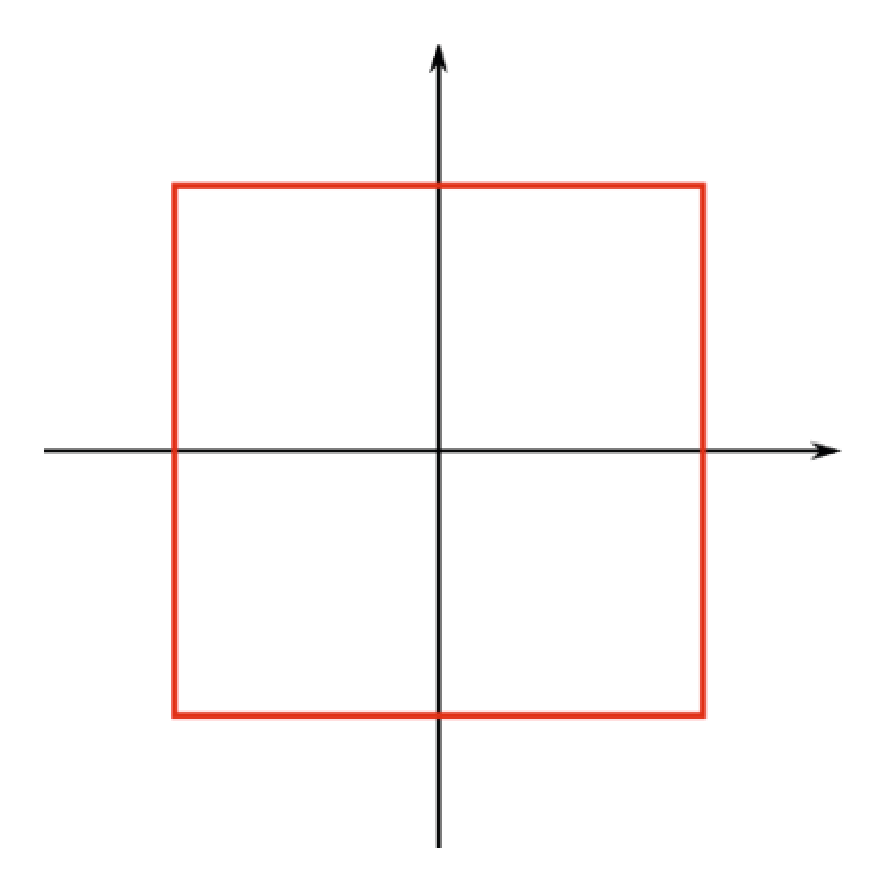
\includegraphics[scale=0.35]{fig3_1} 
		\figcaption{正方形}
	}
	
	\marginpar{
		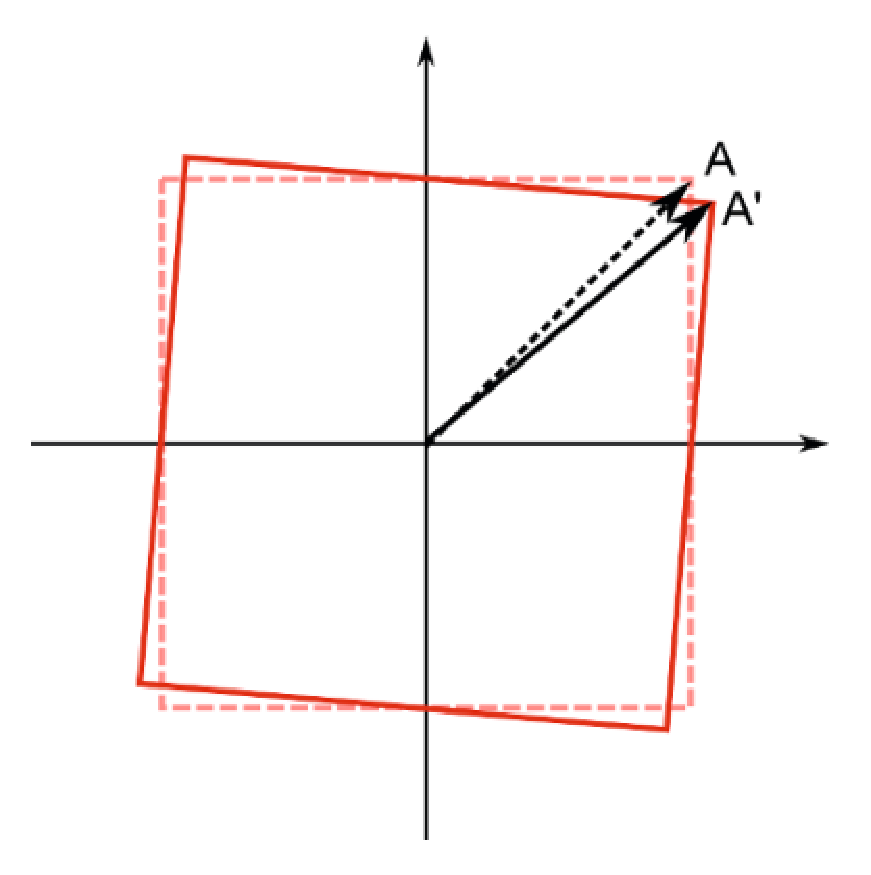
\includegraphics[scale=0.35]{fig3_2.eps}
		\figcaption{正方形绕中心顺时针旋转$5^\circ$}
	}
	
	注意不是所有旋转变换都对称。 我们关注顶点的变化就能看出来, 比如绕中心顺时针旋转$5^\circ$, 这个变换将顶点映射到原来正方形点集之外, 顶点$A$映射到了原来正方形集合之外的点$A'$。 因此这个旋转变换对正方形不具有对称性。 当然, 变换后的点集仍然是个正方形, 但却是不同的正方形(即不同点的集合)。 绕中心转$90^\circ$是对称的, 如图\ref{fig3.3}, 顶点$A$变换到点$B$, 等等, 原来的正方形点集变换到相同的集合。
	
	{
	\centering{
	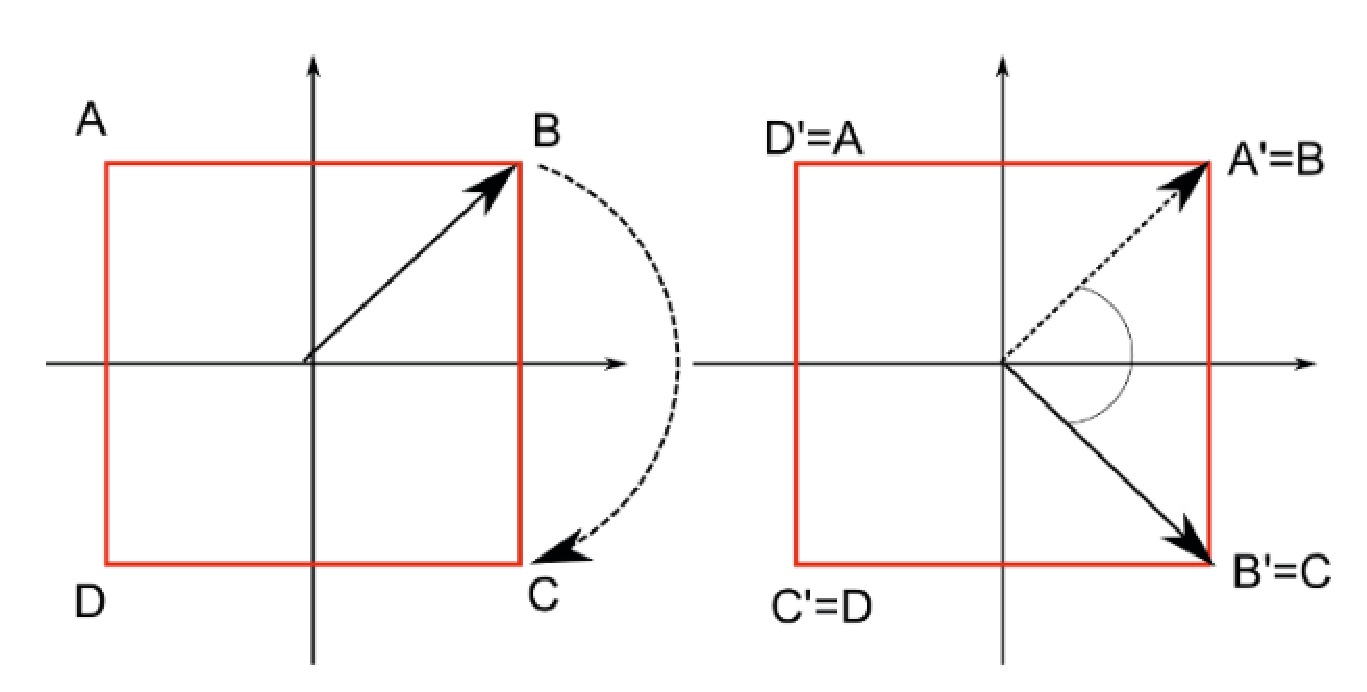
\includegraphics[scale=0.4]{fig3_3}
	\figcaption{正方形绕中心旋转$90^\circ$}
	\label{fig3.3}
	}}
	
	假如你看了一眼原来的正方形, 然后闭上眼睛, 这时有人把正方形做了一个变换。 如果你不能分辨这个正方形是否发生变化, 那么这个变换就是个对称变换。
	
	我们把所有使正方形不变的变换构成的集合称为群。 变换参数(本例中就是旋转角度)不能任意取值(而是取分立的数), 这个群称为离散群。
	
	\item 另一个例子是使单位圆不变的变换构成的集合。 类似地, 单位圆还是一些点构成的集合, 对称变换把这个集合映射到它自身。
	
	单位圆绕圆心旋转任意角度都不变。 换言之, 变换参数(这里就是旋转角度)可以取任意值, 因此这个群称为连续群。
\end{enumerate}
	\marginpar{
		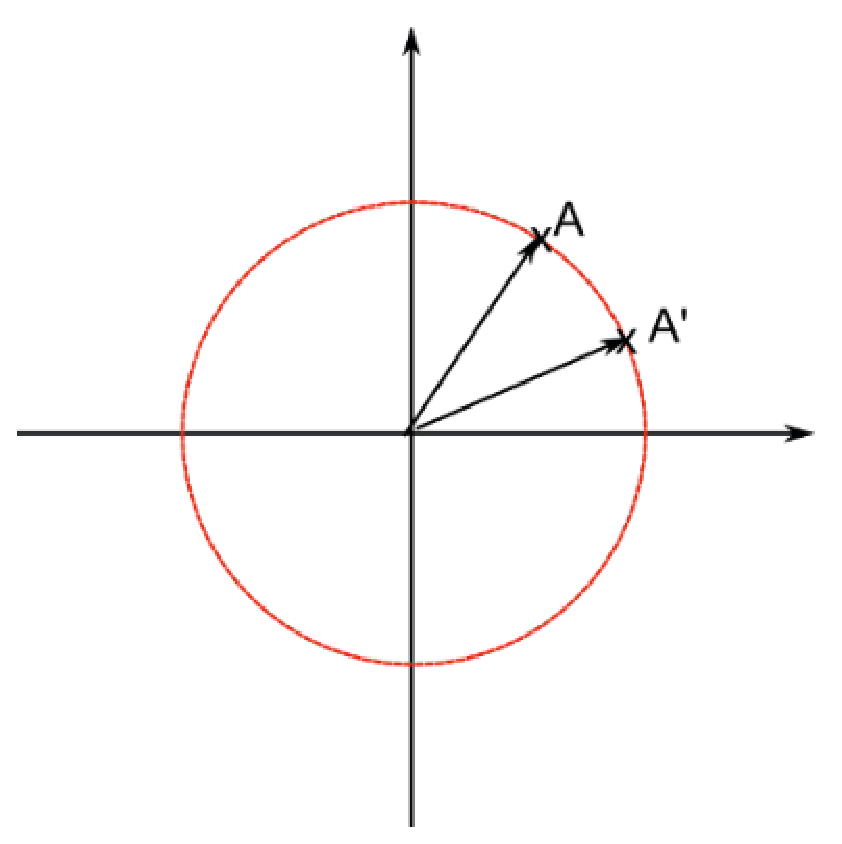
\includegraphics[scale=0.35]{fig3_4.eps}
		\figcaption{单位圆绕圆心旋转任意角度都不变}
	}

数学中除了几何图形之外还有好多别的都有对称性。 例如,对于向量, 我们可以考虑所有让向量长度不变的变换构成的集合。 看出本节开头对称性定义的普遍性了没? 对称性就是变换下的不变性。 非常幸运, 搞数学的早已建立了群论, 它可以研究所有类型的对称性\mpar{历史上数学家们建立群论最初是为了描述方程的对称性}。

为了让描述对称的工具 --- 群 --- 有确切的含义, 我们把对称性的定义用数学语言精炼一下:
\begin{itemize}
	\item 对某物什么也不做(比如转个$0^\circ$)当然也是对称变换(按照我们的对称性定义), 因此任何群都需要包含一个恒等变换(恒等元)。 在上面的例子里, 恒等元就是旋转$0^\circ$。
	
	\item 对某物先做变换再做逆变换的结果必须等于啥也不做。 因此对于群中的任意元素(简称群元), 必须有相应的逆元素。 按定义, 先做变换再做逆变换等于恒等变换。 例如先转$90^\circ$再转$-90^\circ$(先逆针再顺针转)与旋转$0^\circ$相同。
	
	\item 先做一个对称变换再做一个对称变换, 总体效果必须还是对称变换。 例如先旋转$90^\circ$再转$180^\circ$等于直接转$270^\circ$, 后者也是对称变换。 对称变换的这个性质称为封闭性。
	
	\item 对称变换之间必须满足结合律\mpar{它们不一定满足交换律!例如绕不同轴的旋转变换之间不能交换顺序,比如$R_x(\theta) R_z(\phi) \neq R_z(\phi) R_x(\theta)$}。 例如先转$90^\circ$再转$40^\circ$再转$110^\circ$与先转$130^\circ$再转$110^\circ$相同, 先转$90^\circ$再转$150^\circ$也一样。 用符号表示更加清楚:
	\begin{equation}\label{equ3.1}
	R(110^\circ) R(40^\circ) R(90^\circ) = R(110^\circ)\bigg( R(40^\circ)R(90^\circ) \bigg) = R(110^\circ) R(130^\circ)
	\end{equation}
	\begin{equation}\label{equ3.2}
	R(110^\circ) R(40^\circ) R(90^\circ) = \bigg( R(110^\circ) R(40^\circ) \bigg) R(90^\circ) = R(150^\circ) R(90^\circ)
	\end{equation}
	这个性质称为{\bf 结合律}。
	
	\item 我们要有关于两个群元(对称变换)怎样结合的规则, 它是个{\bf 二元运算}\footnote{两个群元结合成一个}, 我们称它为{\bf 群乘法}。
\end{itemize} 
	
	在上面的例子里, 旋转变换的标准表示方法是用旋转矩阵\mpar{旋转矩阵见附录A.2.}, 两个群元(两个旋转矩阵, 或两个旋转操作)结合的规则是线性代数里的矩阵乘法。 同样的变换经常有不同的表示方法\mpar{例如, 二维平面旋转还可以用单位复数描述, 相应的群乘法是复数乘法。 稍后就讨论这一点。}, 群论非常系统性地概括了所有形式。 群论的分支 --- {\bf 表示论}就是研究相同变换的不同描述方式的, 我们在\ref{sec3.5}节学习表示论。

\ 

我们把上述群与对称变换的特征用严谨的数学语言表达, 再将它们提升为公理, 满足这些公理的数学结构就是一个群。必须指出满足群公理的结构可能是超级抽象的, 但我们现在只关注上面例子里的旋转变换那样的群。 \sout{因为我们是物理系的, 而且这是本物理书}

\ 

(我们通过对称变换的性质导出的)群公理\mpar{别担心怎么才能根据这些公理凑出一个群来。 搞物理的往往是从某个变换出发, 考察它是否符合群公理, 如果是\sout{经常是}那么就可以应用群论来解决问题。}: 

一个群是一个集合$G$加上一个定义在$G$上的二元运算(群乘法)$\circ$, 若$(G, \circ)$满足以下公理: 
\begin{itemize}
	\item 封闭性: 对于任意$g_1, g_2 \in G, g_1 \circ g_2 \in G$
	
	\item 单位元: 存在单位元$e \in G$使得对于所有$g \in G, g\circ e = g = e \circ g$
	
	\item 逆元: 对于任意$g \in G$, 存在相应的逆元$g^{-1} \in G$使得$g \circ g^{-1} = e = g^{-1} \circ g$
	
	\item 结合律: 对于任意$g_1, g_2, g_3 \in G, g_1 \circ (g_2 \circ g_3) = (g_1 \circ g_2) \circ g_3$ 
\end{itemize}

总结: 某对象在一些变换下保持不变, 这些变换组成\footnote{我在想这里该用`构成'还是`组成', 后来我觉得无所谓, 因为这不是初中化学...(分子构成物质, 元素组成物质...) --- 译者(SI)}的集合叫做对称群。 对于Minkowski时空, Minkowski度规\mpar{复习一下, Minkowski度规就是在Minkowski空间中用来计算距离和长度的工具, 见第二章。}在变换下保持不变, 相应的对称群称为Poincare群。

要注意群的定义完全与变换的对象是啥没有关系。 我们可以脱离特定对象而只研究对称变换本身, 群的定义将变换从对象中`提取'出来了。 这是非常有用的, 许多不同事物具有同样或同类的对称性。 群论让我们不用管变换的对象(圆还是正方形), 只研究变换(例如旋转)的普遍性质。


\section[二维旋转]{Rotations in two Dimensions\quad 二维旋转}
\label{sec3.2}
我们从一个简单而重要的例子开始学习群论。考虑那些让二维平面中的向量长度不变的对称变换。符合条件的有旋转和反射\mpar{当然还有平移。平移的数学描述与前两者有些不同,我们之后再讨论它。}。它们也是圆的对称变换,一个单位元旋转或反射之后还是单位圆。可见同一个群(对应一种变换)可以作用于不同类对象:圆(几何图形),或者向量。本节考虑向量,可以用旋转矩阵表示向量的旋转或反射\mpar{旋转矩阵的推导见附录A.2.},将起点位于原点的向量绕原点逆时针旋转$\theta$角度的旋转矩阵为:
\begin{equation}
\label{equ3.3}
R_\theta = 
	\begin{pmatrix}
		\cos \theta & \sin \theta \\
		-\sin \theta & \cos \theta
	\end{pmatrix}
\end{equation}

关于$x$轴与$y$轴的反射变换用矩阵表示为:
\begin{equation}
\label{equ3.4}
P_x = 	\begin{pmatrix}
			-1 & 0 \\ 0 & 1
		\end{pmatrix}
\quad
P_y = 	\begin{pmatrix}
			1 & 0 \\ 0 & -1
		\end{pmatrix}
\end{equation}
将矩阵乘法作为群乘法$\circ$, 可以验证$R(\theta), P_x, P_y$与矩阵乘法符合群公理,因而构成一个群,亦即旋转与反射变换构成一个群。

可以用更抽象的方式表达‘所有让二维向量长度不变的变换’,向量长度就是向量与自身点乘的平方根($|a| = \sqrt{a \cdot a}$). 向量长度在变换$a \rightarrow a'$下不变意味着\footnote{等号上面的!只是起强调、提示作用 --- 译者(SI)}:
\begin{equation}
\label{equ3.5}
a' \cdot a' \stackrel{!}{=} a \cdot a
\end{equation}

将变换矩阵记作$\mathcal{O}$,变换即为$a \rightarrow a' = \mathcal{O}a$.
\begin{equation}
\label{equ3.6}
a \cdot a = a^{{T}} a \rightarrow a'^{{T}} a' = (\mathcal{O} a)^{{T}} \mathcal{O} a = a^{{T}} \mathcal{O}^{{T}} \mathcal{O} a \stackrel{!}{=} a^{{T}} a = a \cdot a
\end{equation}
由此可见,使向量长度不变的变换必须满足:
\begin{equation}
\label{equ3.7}
\mathcal{O}^{{T}} \mathcal{O} = I
\end{equation}
其中$I$表示单位矩阵\mpar{ \[I = 
	\begin{pmatrix}
		1 & 0 \\ 0 & 1
	\end{pmatrix}\]}。前文的旋转和反射矩阵都满足此条件\mpar{例如\ref{equ3.3}式的矩阵,
	$R_\theta^{{T}} R = 
	\begin{pmatrix}
		\cos \theta & -\sin \theta \\
		\sin \theta & \cos \theta
	\end{pmatrix}
	\begin{pmatrix}
		\cos \theta & \sin \theta \\
		-\sin \theta & \cos \theta
	\end{pmatrix}
	 = 
	 \begin{pmatrix}
		 \cos^2 \theta + \sin^2 \theta & 0 \\
		 0 & \sin^2 \theta + \cos^2 \theta
	 \end{pmatrix}
	 =
	 \begin{pmatrix}
		 1 & 0 \\ 0 & 1
	 \end{pmatrix}
	$
}%mpar
$2 \times 2$矩阵中所有满足\ref{equ3.7}式的矩阵构成了$\mathcal{O}(2)$群,即所有$2 \times 2$正交矩阵构成的群\mpar{严谨地说,任意$2 \times 2$正交矩阵可以表示为\ref{equ3.3}、\ref{equ3.4}式,或者它们的乘积的形式。}。我们可以找出这个群中描述旋转变换的那一部分(构成一个子群)。根据\ref{equ3.7}式:
\begin{align}
\det(\mathcal{O}^{{T}} O ) = \det(O^{{T}}) \det(O) \stackrel{!}{=} \det(I) = 1 \nonumber\\
\label{equ3.8}
(\det(\mathcal{O}))^2 \stackrel{!}{=} 1 \rightarrow \det{(\mathcal{O})} \stackrel{!}{=} \pm 1
\end{align}

$\det \mathcal{O} = 1$的矩阵对应旋转变换\mpar{见\ref{equ3.3}与\ref{equ3.4}式。反射矩阵的行列式等于$-1$。}。

条件
\begin{align}
\label{equ3.9}
\mathcal{O}^{{T}} \mathcal{O} = I \\
\label{equ3.10}
\det \mathcal{O} = 1
\end{align}
定义了$\mathcal{SO}(2)$群,$\mathcal{S}$表示‘特殊’(special),$\mathcal{O}$表示‘正交’(orthogonal)。

$\mathcal{SO}(2)$包含的旋转变换保持了坐标系的取向,即一个右手坐标系\mpar{右手坐标系与左手坐标系见附录A.5.}经旋转变换后还是右手系,而反射变换会改变它的取向。用线性代数的概念来说,我们规定$\mathcal{SO}(2)$中的矩阵行列式必须为$+1$。

\subsection[单位复数表示旋转变换]{Rotations with Unit Complex Numbers\quad 单位复数表示旋转变换}
\label{sec3.2.1}
还可以用单位复数来表示旋转变换:绕原点旋转$\theta$角可以表示为乘以单位复数$z$(单位复数意为$z = a + ib$,$|z|^2 = z^* z = 1$)\mpar{上标$ ^*$表示复数的共轭复数:$z = a + ib \rightarrow z^* = a - ib$}。

所有单位复数构成一个群,称为\mpar{$\mathcal{U}$表示幺正性,它的含义为$\mathcal{U}^* \mathcal{U} = 1$.}\ $\mathcal{U}(1)$,群乘法即为复数乘法,不难验证它符合群公理。为了看出它与之前引入的$\mathcal{O}(3), \mathcal{SO}(3)$群的关系,我们将$\mathcal{U}(1)$群的条件 --- 单位复数表示为\mpar{定义中包含复数乘法的群的普遍性质见\ref{sec3.10}节的附录。}, $\forall \mathcal{U} \in \mathcal{U}(1)$:
\begin{equation}
\label{equ3.11}
\mathcal{U}^* \mathcal{U} = 1
\end{equation}
单位复数另一种写法是\mpar{附录B.4.2推导了传说中的欧拉公式。对任意复数$z = a + ib$, $a$称为$z$的实部,记为$\mathrm{Re}(z) = a$; $b$称为虚部,记为$\mathrm{Im}(z) = b$. 欧拉公式中$R_\theta$的实部为$\cos  \theta$, 虚部为$\sin \theta$.}:% Euler翻译为欧拉
\begin{equation}
\label{equ3.12}
R_\theta = \mathrm{e}^{i\,\theta} = \cos \theta + i\sin \theta
\end{equation}
$R(\theta)$的模(长度)为:
\begin{equation}
\label{equ3.13}
R_\theta^* R_\theta = \mathrm{e}^{-i\,\theta} \mathrm{e}^{i\,\theta} = \big( \cos \theta - i \sin \theta  \big) \big( \cos \theta + i \sin \theta \big) = 1
\end{equation}

\marginpar{
	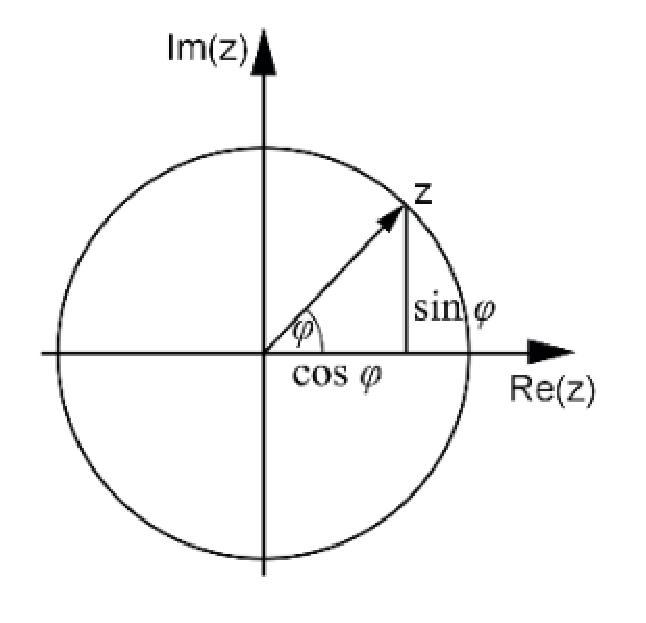
\includegraphics[scale=0.45]{fig3_5.eps} 
	\figcaption{单位复数在复平面的单位圆上}
	}

例:将向量$(3,  5)$对应的复数$z = 3 + 5i$旋转$90^\circ$:
\begin{equation}
\label{equ3.14}
z \rightarrow z' = \mathrm{e}^{i\, 90^\circ}z = \bigg( \underbrace{\cos 90^\circ}_{=0} + i\underbrace{\sin 90^\circ}_{=1} \bigg) (3 + 5i) = i(3 + 5i) = 3i - 5
\end{equation}

图3.6绘制了旋转前后的向量(复数),图中可见复数乘以$\mathrm{e}^{i\, 90^\circ}$旋转了$90^\circ$.
\marginpar{
	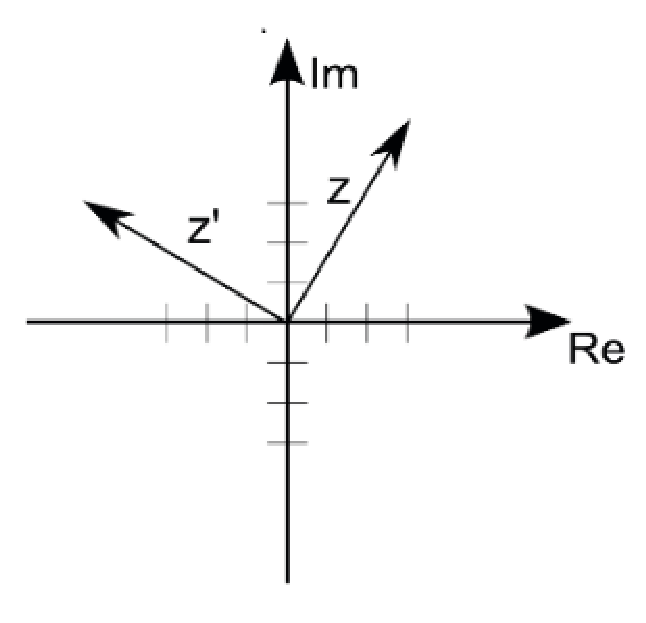
\includegraphics[scale=0.45]{fig3_6.eps} 
	\figcaption{复数通过乘以单位复数进行旋转}
	}
需要注意$\mathrm{e}^{i\, 90^\circ}$作用于(乘以)向量对应的复数而非向量本身。描述二维旋转只需要一个参数:旋转角$\phi$. 而复数有两个自由度(实部和虚部),因此我们加上单位复数的限制:$|z| = \text{实部}^2 + \text{虚部}^2 = 1$,刚好只剩一个自由度。

描述二维旋转的两种方式 --- 单位复数与$2 \times 2$矩阵(矩阵元都是实数)通过如下方式相联系。定义:
\begin{equation}
\label{equ3.15}
\mathbf{1} = 
	\begin{pmatrix}
		1 & 0 \\ 0 & 1
	\end{pmatrix}
,\quad
\mathbf{i} = 
	\begin{pmatrix}
		0 & -1 \\ 1 & 0
	\end{pmatrix}
\end{equation}
不难验证这样定义的$\mathbf{1, i}$仍然满足:
\begin{equation}
\mathbf{1}^2 = \mathbf{1},\quad \mathbf{i}^2 = -\mathbf{1},\quad \mathbf{1i} = \mathbf{i1} = \mathbf{i}
\end{equation}
这样单位复数对应的$2 \times 2$实数矩阵为\footnote{原文此式有误,译文已参照勘误表修改。}
\begin{equation}
\label{equ3.17}
R_\theta = \cos \theta + i\sin\theta = \cos \theta 
\begin{pmatrix}
	1 & 0 \\ 0 & 1
\end{pmatrix}
+ \sin \theta
\begin{pmatrix}
	0 & -1 \\ 1 & 0
\end{pmatrix}
=
\begin{pmatrix}
	\cos \theta & -\sin \theta \\
	\sin \theta & \cos \theta
\end{pmatrix}
\end{equation}
可见,定义了复单位$i \rightarrow \text{实矩阵}$的对应关系后,单位复数就回到了熟悉的旋转矩阵。还有一点要注意:旋转矩阵作用于向量(列矩阵),而我们将$i$与$2 \times 2$矩阵相联系,因此被旋转的向量(与一个复数对应)也将变成一个$2 \times 2$矩阵。

例:任意向量$(a, b)$对应的复数对应的$2 \times 2$矩阵为:
\begin{equation}
\label{equ3.18}
z = a + ib = a
\begin{pmatrix}
	1 & 0 \\ 0 & 1
\end{pmatrix}
+ b
\begin{pmatrix}
	0 & -1 \\ 1 & 0
\end{pmatrix}
=
\begin{pmatrix}
	a & -b \\ b & a
\end{pmatrix}
\end{equation}
将旋转矩阵作用于$z$:
\begin{eqnarray}
\label{sec3.19}
	z' &=& \begin{pmatrix}
			a' & -b' \\ b' & a'
		 \end{pmatrix}
	= R_\theta z = 
		\begin{pmatrix}
			\cos \theta & -\sin \theta \\
			\sin \theta & \cos \theta
		\end{pmatrix}
		\begin{pmatrix}
			a & -b \\ b & a
		\end{pmatrix}
	\nonumber \\
	&=& \begin{pmatrix}
			a\cos\theta - b\sin \theta & - b\cos \theta - a \sin \theta \\
			a\sin \theta + b\cos \theta & -b \sin \theta + a \cos \theta
		\end{pmatrix}
\end{eqnarray}
由上式可得
\begin{align}
\label{equ3.20}
a' &= a \cos \theta - b \sin \theta \\
\label{equ3.21}
b' &= a \sin \theta + b \cos \theta
\end{align}
这与旋转矩阵作用于向量(列矩阵形式)相同:
\begin{equation}
\label{equ3.22}
	\begin{pmatrix}
		\cos \theta & -\sin \theta \\
		\sin \theta & \cos \theta
	\end{pmatrix}
	\begin{pmatrix}
		a \\ b
	\end{pmatrix}
	=
	\begin{pmatrix}
		a \cos \theta - b \sin \theta \\
		a \sin \theta + b \cos \theta
	\end{pmatrix}
	=
	\begin{pmatrix}
		a' \\ b'
	\end{pmatrix}
\end{equation}
我们看到这两种表示方法是一回事儿,用数学术语来说,$\mathcal{SO}(2)$与$\mathcal{U}(1)$间有一个同构映射\mpar{如果映射$\Pi: G \rightarrow G'$是一一映射,并且满足:$\forall g_1, g_2 \in G, \Pi(g_1) \circ \Pi(g_2) = \Pi(g_1 \circ g_2)$, 则$\Pi$就是同构映射,并且称群$G, G'$是同构的。}。这一点太重要了,之后的篇幅会不断出现这种思想。

下面研究三维旋转,尝试找出它的两种描述方法\mpar{其中蕴含着十分硬却失挺(interesting)的内容... 与二维旋转类似,我们将找出三维旋转的第二法,这个第二法能够揭示大自然更深刻的内容。}。

\section[三维旋转]{Rotations in three Dimensions\quad 三维旋转}
\label{sec3.3}
三维向量旋转变换当然可以用$3 \times 3$旋转矩阵\footnote{原文公式有误,译文已按勘误表改正。}:
\begin{align}
R_x =
	\begin{pmatrix}
		1 & 0 & 0 \\
		0 & \cos \theta & -\sin \theta \\
		0 & \sin \theta & \cos \theta
	\end{pmatrix}
\quad
R_y = 
	\begin{pmatrix}
		\cos \theta & 0 & \sin \theta \\
		0 & 1 & 0 \\
		-\sin \theta & 0 & \cos \theta
	\end{pmatrix}
\nonumber \\
\label{equ3.23}
R_z =
	\begin{pmatrix}
		\cos \theta & -\sin \theta & 0 \\
		\sin \theta & \cos \theta & 0 \\
		0 & 0 & 1
	\end{pmatrix}
\end{align}
类比$\mathcal{SO}(2)$群,上面三个矩阵构成了$\mathcal{SO}(3)$群的一组基\mpar{基的概念见附录A.1.}。这意味着$\mathcal{SO}(3)$中的任意群元(矩阵)都可以写为$R_x, R_y, R_z$的线性组合,且系数唯一。
将向量
\begin{equation*}
\vec{v} = \begin{pmatrix}
			1 \\ 0 \\ 0
		\end{pmatrix}
\end{equation*}
绕$z$轴旋转\mpar{三维向量旋转的一般情况的推导见附录A.2.}就是用旋转矩阵乘以向量:
\begin{equation}
\label{equ3.24}
R_z(\theta) \vec{v} = 
	\begin{pmatrix}
		\cos \theta & -\sin \theta & 0 \\
		\sin \theta & \cos \theta & 0 \\
		0 & 0 & 1
	\end{pmatrix}
	\begin{pmatrix}
		1 \\ 0 \\ 0
	\end{pmatrix}
=
	\begin{pmatrix}
		\cos \theta \\ \sin \theta \\ 0
	\end{pmatrix}
\end{equation}
为找出描述三维旋转的第二法,我们尝试把复数的概念扩展到三维空间。首先试着把$2$维的复数\footnote{实部虚部两个自由度}扩展为$3$维复数,但前人探索发现没有$3$维的,但存在$4$维‘复数’,称为{\bf 四元数(quaternions)}。下面就会看到四元数正是描述三维旋转的第二法,并且它还能深刻揭示宇宙 --- 四维时空的规律。描述三维旋转需要三个参数(绕$x,y,z$轴的旋转角),而四元数有四个参数,这与二维旋转的情况类似\mpar{单位复数描述二维旋转。}。四元数加上单位长度的限制 --- 单位四元数(三个自由参数)能够描述三维旋转。

\subsection[四元数]{Quaternions\quad 四元数}
\label{sec3.3.1}
我们类比复数来构造四元数,复数只有一个虚单位$i$,而四元数里定义三个虚单位,记作$\mathbf{i,j,k}$,它们仍然满足
\begin{equation}
\label{equ3.25}
\mathbf{i}^2 = \mathbf{j}^2 = \mathbf{k}^2 = -1
\end{equation}
这样任意一个四元数$q$表示为
\begin{equation}
\label{equ3.26}
q = a\mathbf{1} + b\mathbf{i} + c\mathbf{j} + d\mathbf{k}
\end{equation}
其中$a, b, c, d \in \mathbb{R}$, $\mathbf{1}$就是正常的实数1。\footnote{$\mathbf{1,i,j,k}$用黑体表示是为了强调它们是四元数的基。---译者(SI)}

要想定义四元数间的乘法,必须定义虚单位间的乘法规则,比如$\mathbf{ij} = ?$. 为此再定义
\begin{equation}
\label{equ3.27}
\mathbf{ijk} = -1
\end{equation}
这样虚单位间的乘法就没问题了,例如,为导出$\mathbf{ij} = \mathbf{k}$, 在\ref{equ3.27}式等号两侧右乘$\mathbf{k}$:
\begin{equation}
\label{equ3.28}
\mathbf{ij} \underbrace{\mathbf{kk}}_{= -1} = -\mathbf{k} \rightarrow \mathbf{ij} = \mathbf{k}
\end{equation}

单位四元数$q = a\mathbf{1} + b\mathbf{i} + c\mathbf{j} + d\mathbf{k}$满足\mpar{符号$\dag$称为`dagger',表示转置加取复共轭,即$a^\dag = (a^*)^T$。实数向量间的点乘定义为$a \cdot b = a^T b$, 向量用列矩阵表示,其转置为行矩阵,于是点乘的定义符合矩阵乘法规则。四元数对应的列矩阵含复数,为使四元数与它自身相乘结果为实数(实数结果可表示‘长度’),在转置之外还加上取复共轭。}:
\begin{align}
q^\dag q &\stackrel{!}{=} 1 \nonumber\\
\label{equ3.29}
\rightarrow (a\mathbf{1} - b\mathbf{i} - c\mathbf{j} - d\mathbf{k}) (a\mathbf{1} +& b\mathbf{i} + c\mathbf{j} + d\mathbf{k}) = a^2 + b^2 + c^2 + d^2 \stackrel{!}{=} 1
\end{align}

就像单位复数构成一个群(群乘法为复数乘法)那样,单位四元数也构成一个群(群乘法为四元数乘法)。

类似于我们将二维复数与$2 \times 2$实数矩阵建立联系的做法,四元数也可如此 --- 将四个基$\mathbf{1,i,j,k}$与合适的矩阵一一对应。其中一种方式(还有别的方式)是将它们与$2 \times 2$复数矩阵对应:
\begin{align}
\mathbf{1} = \begin{pmatrix}
				1 & 0 \\ 0 & 1
			 \end{pmatrix}
\quad &, \quad
\mathbf{i} = \begin{pmatrix}
				0 & -1 \\ 1 & 0 
			 \end{pmatrix}
\nonumber \\
\label{equ3.30}
\mathbf{j} = \begin{pmatrix}
				0 & -i \\ -i & 0
			 \end{pmatrix}
\quad &, \quad
\mathbf{k} = \begin{pmatrix}
				i & 0 \\
				0 & -i
			 \end{pmatrix}
\end{align}
不难验证上式满足四元数乘法,比如\ref{equ3.25}、\ref{equ3.27}式。这样任意一个四元数都可用矩阵表示为:
\begin{equation}
\label{equ3.31}
q = a\mathbf{1} + b\mathbf{i} + c\mathbf{j} + d\mathbf{k} = \begin{pmatrix}
	a + di & -b - ci \\
	b - ci & a - di
	\end{pmatrix}
\end{equation}
由上式可见
\begin{equation}
\label{equ3.32}
\det(q) = a^2 + b^2 + c^2 + d^2
\end{equation}
上式与\ref{equ3.29}式比较可以发现单位四元数对应的矩阵的行列式为$1$。因此单位四元数对应的$2 \times 2$复数矩阵$\mathcal{U}$满足:
\begin{equation}
\label{equ3.33}
\mathcal{U}^\dag \mathcal{U} = 1, \quad \text{且} \det(\mathcal{U}) = 1
\end{equation}
注意\ref{equ3.30}式中的矩阵是线性独立的\mpar{线性独立的概念见附录A.1.},它们构成群$\mathcal{SU}(2)$的基。与之前相同,$\mathcal{S}$表示特殊(special),含义为$\det (\mathcal{U}) = 1$;$\mathcal{U}$表示幺正(unitary)\mpar{进一步介绍见本章附录 --- \ref{sec3.10}节。},即$\mathcal{U}^\dag \mathcal{U} = 1$。任意单位四元数都唯一对应$\mathcal{SU}(2)$群中的一个群元。

$\mathcal{SU}(2)$群如何与三维旋转联系?事情正在起变化,$\mathcal{SU}(2)$群与$\mathcal{SO}(3)$\mpar{$\mathcal{SO}(3)$群就是三维旋转矩阵构成的群。}之间的对应关系并不像二维旋转中$\mathcal{U}(1)$与$\mathcal{SO}(2)$那样简单。

2维虚数$z = a + ib$与2维向量很容易对应。单位复数保证了矢量长度在旋转变换下不变\mpar{注意这里的$R$表示一个单位复数,即$R^* R = 1$, $R$与复数$z$相乘就将$z$进行旋转变换。}:$(Rz)^* Rz = z^* R^* Rz = z^* z$。四元数有$4$个参数,它与三维向量的对应关系是并不明显。我们尝试将三维向量$\vec{v} = (x, y, z)$定义为如下四元数\footnote{注意下式中的$\mathbf{ijk}$是四元数的‘基’而非三维直角坐标系的基矢。 --- 译者}:
\begin{equation}
\label{equ3.34}
v \equiv x\mathbf{i} + y\mathbf{j} + z\mathbf{k}
\end{equation}
利用前述四元数的矩阵表示可得:
\begin{equation}
\label{equ3.35}
\det(v) = x^2 + y^2 + z^2
\end{equation}
于是保持向量$(x, y, z)$长度不变的变换就对应于保持矩阵行列式不变的矩阵变换。而{\bf 单位}四元数对应矩阵都具有{\bf 单位}行列式,它与任意矩阵相乘不改变该矩阵的行列式\footnote{利用$\det(AB) = \det(A)\det(B)$, --- 译者}。进展很顺利,但现在有个微妙的状况:继续猜想下去,我们会认为用单位四元数$u$旋转向量(对应的四元数)$v$直接用$u$乘以$v$就可以了(按照四元数乘法规则)。但细想起来这却不行,因为根据\ref{equ3.34}式,我们把任意三维向量对应的四元数定义在$\mathbb{R}\mathbf{i} + \mathbb{R}\mathbf{j} + \mathbb{R}\mathbf{k}$的范围内,$u$与$v$的四元数乘积会超出这个范围,这样向量旋转后可能不是个向量!这当然不行。

事实上,旋转变换表示为:
\begin{equation}
\label{equ3.36}
v' = q^{-1} v q
\end{equation}
其中$v$, $v'$分别为旋转前后的向量,$q$为表示旋转的单位四元数。

这样我们终于实现了描述三维旋转的第二法 --- 单位四元数。

例:定义$u$是$\mathbb{R}\mathbf{i} + \mathbb{R}\mathbf{j} + \mathbb{R}\mathbf{k}$中的某一单位向量,则任意单位四元数$t$可表示为:
\begin{equation}
\label{equ3.37}
t = \cos \theta +  u\sin \theta
\end{equation}
利用\ref{equ3.34}式,任意三维向量$\vec{v}$可表示为:
\begin{equation}
\label{equ3.38}
\vec{v} = (v_x, v_y, v_z)^T = v_x \mathbf{i} + v_y \mathbf{j} + v_z \mathbf{k} \underbrace{=}_{\ref{equ3.31}\text{式}} \begin{pmatrix}
		iv_z & -v_x - iv_y \\
		v_x - iv_y & -iv_z
	\end{pmatrix}
\end{equation}

简明起见我们举个特例,把向量$\vec{v} = (1, 0, 0)^T$绕$z$轴旋转。
\begin{align}
\label{equ3.39}
\vec{v} &= (1, 0, 0)^T \rightarrow v = 1\mathbf{i} + 0\mathbf{j} + 0\mathbf{k} = 
	\begin{pmatrix}
		0 & -1 \\ 1 & 0
	\end{pmatrix}
\\
\label{equ3.40}
R_z(\theta) &= \cos \theta \mathbf{1} + \sin \theta \mathbf{k} =
	\begin{pmatrix}
		\cos \theta + i\sin \theta & 0 \\
		0 & \cos \theta - i\sin \theta
	\end{pmatrix}
\end{align}
上式也可用欧拉公式写出\mpar{欧拉公式的推导见附录B.4.2}:
\begin{equation}
\label{equ3.41}
\mathrm{e}^{ix} = \cos x + i\sin x
\Rightarrow
R_z(\theta) = \begin{pmatrix}
				\mathrm{e}^{i\theta} & 0 \\
				0 & \mathrm{e}^{-i\theta}
			  \end{pmatrix}
\end{equation}
四元数旋转矩阵的逆矩阵为:
\begin{equation}
\label{equ3.42}
R_z^{-1} (\theta) = 
	\begin{pmatrix}
		\cos \theta - i\sin \theta & 0 \\
		0 & \cos \theta + i\sin \theta
	\end{pmatrix}
=
	\begin{pmatrix}
		\mathrm{e}^{-i\theta} & 0 \\
		0 & \mathrm{e}^{i\theta}
	\end{pmatrix}
\end{equation}
根据\ref{equ3.36}式旋转向量$v$;
\begin{align}
v' &= R_z^{-1} (\theta) v R_z(\theta) =
	\begin{pmatrix}
		\mathrm{e}^{-i\theta} & 0 \\
		0 & \mathrm{e}^{i\theta}
	\end{pmatrix}
	\begin{pmatrix}
	0 & -1 \\ 1 & 0
	\end{pmatrix}
	\begin{pmatrix}
		\mathrm{e}^{i\theta} & 0 \\
		0 & \mathrm{e}^{-i\theta}
	\end{pmatrix}
\nonumber \\
\label{equ3.43}
&= \begin{pmatrix}
		0 & -\mathrm{e}^{-i 2\theta} \\
		\mathrm{e}^{i 2\theta} & 0
	\end{pmatrix}
= \begin{pmatrix}
		0 & -\cos (2\theta) + i\sin (2\theta) \\
		\cos (2\theta) + i\sin (2\theta) & 0
  \end{pmatrix}
\end{align}
另一方面,向量$v'$用四元数表示为:
\begin{equation}
\label{equ3.44}
v' = 
	\begin{pmatrix}
		iv'_z & -v'_x - iv'_y \\
		v'_x - iv'_y & -iv'_z
	\end{pmatrix}
\end{equation}
上式与\ref{equ3.43}式比较可得:
\begin{equation}
\label{equ3.45}
v'_x = \cos(2\theta),\quad v'_y = -\sin (2\theta),\quad v'_z = 0
\end{equation}
所以
\begin{equation}
\label{equ3.46}
\rightarrow \vec{v'} = \big( \cos(2\theta), -\sin (2\theta), 0 \big)^T
\end{equation}
由上式可见从$\vec{v}$到$\vec{v}'$确实进行了旋转\mpar{见\ref{equ3.24}式,那里我们用三维旋转矩阵旋转向量。},但是要注意,上式表示我们没有把$\vec{v}$旋转$\theta$角度,而是旋转了$2\theta$!因此我们定义$\phi \equiv 2 \theta$, 这样$\phi$表示真正的旋转角,$\ref{equ3.37}$重写为:
\begin{equation}
\label{equ3.47}
t = \cos \left( \frac{\phi}{2} \right) + \sin \left(\frac{\phi}{2} \right) u
\end{equation}

这样定义的单位四元数与三维旋转矩阵之间的关系并非一一对应的,而是两个单位四元数描述同一个旋转,例如\mpar{将向量旋转$\pi$与旋转$3\pi = \pi + 2\pi$相同。换言之:两个单位四元数$u$与$-u$对应同一变换:旋转$\pi$.}:

{
\centering
\setlength{\unitlength}{0.8cm}
\begin{picture}(6, 4.5)\thicklines
\put(0.5, 3){\makebox(2.5, 1.2){\text{$t_{\phi = \pi} = u$}}}
\put(5.5, 3){\makebox(2.5, 1.2){\text{$t_{\phi = 3\pi} = -u$}}}

\put(1.7, 3.2){\vector(1, -1){1.4}}
\put(6.0, 3.2){\vector(-1, -1){1.4}}
\put(2.8, 0.8){\makebox(2.5, 1.2){\text{将向量旋转$\pi$}}}
\end{picture}
}

因此$\mathcal{SU}(2)$群称为$\mathcal{SO}(3)$群的{\bf 双覆盖}。一个$\mathcal{SU}(2)$中的群元对应$\mathcal{SO}(3)$的哪个群元是很明确的,反过来就不行,因为$\mathcal{SO}(3)$中的一个群元对应$\mathcal{SU}(2)$中的两个。这并非仅有数学意义,稍后就会看到,在物理上,一个能覆盖别的群的群往往更加深刻\mpar{剧透:Lorentz群的双覆盖蕴含{\bf 自旋}概念,而Lorentz群自身并不具有。自旋是指粒子的某种内禀角动量,它是粒子最重要的特征之一。自旋在小节\ref{sec4.5.4}和\ref{sec8.5.5}详述。}。

给定某个群,为了找出能覆盖这个群的群,我们需要学习Lie代数 --- Lie理论的利器,下一节就讲Lie代数。

注意我们把三维向量对应到四元数集$\mathbb{R}\mathbf{i} + \mathbb{R}\mathbf{j} + \mathbb{R}\mathbf{k}$中,因此四元数的一个参数没有用到,这是相对论的伏笔。比如将时间$t$考虑进来后,四维‘向量’与四元数对应的十分自然,就像二维复数与二维向量之间那样:$v = t\mathbf{1} + x\mathbf{i} + y\mathbf{j} + z\mathbf{k}$。纯数学的观点鼓励我们使用4维向量。如果我们想描述四维旋转(因为我们目前认为宇宙是$3+1$四维时空),应该怎么办?有两个选择:
\begin{itemize}
	\item 再去找更高维的‘复数’,或者:
	\item 再用四元数试试看。
\end{itemize}
从刚才的遐想可以看出四元数与四维旋转有着暧昧的联系。任意四维旋转需要$6$个参数表示\mpar{四维旋转矩阵$\mathcal{O}$($4 \times 4$)有$16$个参数,条件$\mathcal{O}^T \mathcal{O} = 1$与$\det(\mathcal{O}) = 1$将$16$个参数限制为$6$个自由参数。},没有$7$维复数,这样‘单位7维复数描述6个参数的四维旋转’就行不通了。我们注意到{\bf 两个}单位四元数正好有$6$个自由参数。因此两个单位四元数很可能可以描述四维旋转。之后会看到,两个$\mathcal{SU}(2)$群与四维旋转群确实存在千丝万缕的联系。

\section[Lie代数]{Lie Algebras\quad Lie代数}
\label{sec3.4}
Lie理论是研究连续对称的理论。连续对称的例子可见本章开头讨论的单位圆的旋转对称性。连续性意味着存在无限接近于恒等变换(恒等变换:什么都不干)的群元。相对的,离散群的群元个数是可数的,不存在无限接近于恒等元的群元。例如把正方形绕中心转$0.000001^\circ$,这与恒等变换(转$0^\circ$)非常接近,但它不是正方形的恒等变换。而把圆绕圆心转$0.000001^\circ$就是对称的。圆的对称群(对称变换组成的群)是连续的,因为变换参数(旋转角)可以取任意(连续)的值。用数学符号来表示:把恒等元记作$I$,无限接近恒等元的群元$g$可表示为:
\begin{equation}
\label{equ3.48}
g(\epsilon) = I + \epsilon X
\end{equation}
其中$\epsilon$表示小量(数学总是用$\epsilon$表示小量),$X$称为生成元,稍后就讨论它。这样一个轻微的小变换作用在对象上几乎啥也不变,有时称$g(\epsilon)$为无穷小变换。把无穷小变换重复许多次就能得到一个有限大小的变换。以旋转为例:许多朝同一方向小旋转等效于一次有限大的旋转。用数学语言来说,我们可以将无穷小变换重复许多次:
\begin{equation}
\label{equ3.49}
h(\theta) = \underbrace{(I + \epsilon X)(I + \epsilon X) \dots (I + \epsilon X)}_{k\text{个}(I + \epsilon X)} = (I + \epsilon X)^k
\end{equation}
其中$k$表示无穷小变换重复的次数。如果$\theta$表示有限大的旋转角,比如$50^\circ$什么的,然后$N$表示超大的数,则无限接近于恒等变换的旋转变换可表示为:
\begin{equation}
\label{equ3.50}
g(\frac{\theta}{N}) = I + \frac{\theta}{N} X
\end{equation}
要使上式表示的变换尽可能小,则让$N$尽可能大,令$N \rightarrow \infty$。为了从这样一个无穷小变换得到一个有限变换,需要把无穷小变换重复无限多次,即:
\begin{equation}
\label{equ3.51}
h(\theta) = \lim_{N \rightarrow \infty} \left( I + \frac{\theta}{N}X \right)^N
\end{equation}
微积分告诉我们这个极限就是指数函数\mpar{\ref{equ3.51}式经常用作指数函数的定义。指数的级数表示与\ref{equ3.51}式等价性的证明见附录B.4.1. 这在几乎所有的数学分析课本中都能找到。}:
\begin{equation}
\label{equ3.52}
h(\theta) = \lim_{N \rightarrow \infty} \left( I + \frac{\theta}{N}X \right)^N = \mathrm{e}^{\theta X}
\end{equation}
上式有$X$生成了有限变换$h(\theta)$的感觉,因此$X$成为{\bf 生成元}。生成元的严格定义之后详述,下面先从另一个角度看这个问题。

考虑某个用矩阵表示的连续变换群,对任意群元,在恒等元$I$处做Taylor展开\mpar{如果你从未听说过Taylor展开或Taylor级数,作者推荐你看一看附录B.3. }。
\begin{equation}
\label{equ3.53}
h(\theta) = I + \frac{dh}{d\theta} \Bigg|_{\theta = 0} \theta + \frac{1}{2} \frac{d^2 h}{d \theta^2} \Bigg|_{\theta = 0} \theta^2 + \dots = \sum_n \frac{1}{n!} \frac{d^n h}{d \theta^n} \Bigg|_{\theta = 0} \theta^n
\end{equation}

利用指数函数的级数展开可将上式的级数表示为更紧凑的形式\mpar{附录B.4.1中有推导}:
\begin{equation}
\label{equ3.54}
h(\theta) = \exp \left( \frac{dh}{d\theta}\Big|_{\theta = 0} \theta \right) \equiv \sum_n \frac{1}{n!} \frac{d^n h}{d \theta^n}\Bigg|_{\theta = 0} \theta^n
\end{equation}
这与之前的描述有联系。比较上式与\ref{equ3.52}式可得:
\begin{equation}
\label{equ3.55}
X = \frac{dh}{d\theta}\Bigg|_{\theta = 0}
\end{equation}

蕴含在上述推导中的思想是:通过研究群中重要的无穷小元素 --- {\bf 生成元}\footnote{注意生成元$X$并非群元,$I + \epsilon X$才是。}(上面的$X$)就能获得群的许多重要信息。

矩阵Lie群(记作$G$)的Lie代数就是下面的集合:
\[ 
\Big\{X \Big| \text{若}\mathrm{e}^X \in G \Big\}
\]
即如果$X$满足$\mathrm{e}^X$是$G$的群元,则$X$就是$G$的Lie代数(它是一个集合!)中的元素。这个简单定义只对矩阵Lie群管用。之后我们引入Lie代数的一般定义。

上面的矩阵Lie群的Lie代数的定义用数学语言表述为\mpar{群$G$的Lie代数通常用哥特体活字(Fraktur)字母$\mathfrak{g}$表示。}:

{ \it
$n \times n$矩阵Lie群$G$的Lie代数$\mathfrak{g}$是满足如下条件的$n \times n$矩阵$X$的集合:

	{\begin{center}
		$\mathrm{e}^{tX} \in G, t \in \mathbb{R}$
	\end{center}
	}
}

根据群的定义,群无非是一些变换的集合。群乘法$\circ$告诉我们群元之间怎样结合。矩阵Lie群的群乘法就是矩阵乘法,我们可能naive地认为Lie代数的元素之间采用相同的方式结合($\circ$),但这并不正确!诚然,(矩阵Lie群的)Lie代数的元素都是矩阵\mpar{Lie群理论的著名定理 --- Ado定理(Ado's Theorem)告诉我们任意Lie代数与矩阵Lie代数同构。
},但两个Lie代数的矩阵乘法的结果往往不再是Lie代数的元素。Lie代数元素间有另外的结合规则,当然它与原来群的群乘法直接有关。

Lie群乘法与Lie代数结合法则之间的关系由著名的Baker-Campbell-Hausdorff公式(以下简称BCH公式)给出\mpar{我们不讲这个公式的证明,在大多数关于Lie理论的教材都能找到,比如 William Fulton and Joe Harris. Representation Theory: A First Course. Springer, 1st corrected edition, 8 1999. ISBN 9780387974958}:
\begin{equation}
\label{equ3.56}
\mathrm{e}^X \circ \mathrm{e}^Y = \mathrm{e}^{X + Y + \frac{1}{2}[X, Y] + \frac{1}{12} \big[X, [X, Y]\big] - \frac{1}{12} \big[Y, [X, Y]\big] + \dots  }
\end{equation}
其中\mpar{重复一下,群$G$的Lie代数通常用哥特体字母$\mathfrak{g}$表示。}$X, Y \in \mathfrak{g}$, 即$X, Y$是群$G$的生成元。$\mathrm{e}^X, \mathrm{e}^Y$是$G$的群元,把它们分别记作$g, h$,这样上式写成:
\begin{equation}
\label{sec3.57}
\underbrace{g}_{\in G} \circ \underbrace{h}_{\in G} = \mathrm{e}^X \circ \mathrm{e}^Y = \underbrace{\mathrm{e}^{ X + Y + \frac{1}{2} [X, Y] + \frac{1}{12}\big[X, [X, Y]\big] - \frac{1}{12} \big[Y, [X, Y]\big] + \dots }}_{\in G}
\end{equation}

上式等号右侧是群的一个群元,可见两个群元($g,h$)相乘可表示为一些Lie代数元素的和(再取指数)。上两式出现的新运算$[,]$称为{\bf Lie括号},对于矩阵Lie群,$[X, Y] = XY - YX$,$[X, Y]$称为$X, Y$的对易子。注意$XY$和$YX$一般不是Lie代数的元素,但它们的差一定是\mpar{John Stillwell. Naive Lie Theory. Springer, 1st edition, August 2008a. ISBN 978-0387782140 里面有漂亮的证明。}!

由BCH公式可知Lie代数元素间的乘法规则是Lie括号$[,]$,而非最初认为的矩阵乘法。就像群在群乘法$\circ$运算(矩阵群的$\circ$就是矩阵乘法)下封闭那样,我们称Lie代数在Lie括号运算下封闭。集合在某运算下封闭的含义是集合的任意两个元素进行该运算所得结果仍在此集合内\mpar{用数学语言表示封闭性:$\forall g, h \in G$, $g \circ h \in G$。 对于$X, Y \in \mathfrak{g}, [X, Y] \in \mathfrak{g}, X \circ Y \notin \mathfrak{g}$}。

在学习一个Lie代数的例子之后,我们将讨论Lie代数的现代定义。现代定义是从群的生成元在Lie括号运算下的行为来定义的。利用更广泛的现代定义就能看出哪些不同的群具有{\bf 相同的}Lie代数,只从上面的Lie代数定义出发看不出这一点来。因此Lie代数的新定义能让我们更深刻地认识一种变换的基本特征。同一Lie代数可对应许多Lie群,Lie理论的一条重要定理告诉我们这其中有一个{\bf 特别的}Lie群。引入Lie群的现代定义之后上面所说的就具体起来了。

下面我们就举一个从给定的群导出相应Lie代数的例子。

\subsection[$\mathcal{SO}(3)$群的生成元与Lie代数]{The Generators and Lie Algebra of $\mathcal{SO}(3)$\quad $\mathcal{SO}(3)$群的生成元与Lie代数}
\label{sec3.4.1}
$\mathcal{SO}(3)$群的定义为(\ref{equ3.10}式):
\begin{equation}
\label{equ3.58}
\mathcal{O}^T \mathcal{O} \stackrel{!}{=} I , \quad \det(\mathcal{O}) \stackrel{!}{=} 1
\end{equation}

任意群元$\mathcal{O}$用相应的生成元$J$表示为:
\begin{equation}
\label{equ3.59}
\mathcal{O} = \mathrm{e}^{\phi J} % 这里似乎应该用\phi(原文为\Phi),因为(3.69)式是用\phi表示的
\end{equation}

上式带入群的第一个定义条件得:
\begin{equation}
\label{equ3.60}
\mathcal{O}^T \mathcal{O} = \mathrm{e}^{\phi J^T} \mathrm{e}^{\phi J} \stackrel{!}{=} 1 \quad \rightarrow \quad J^T + J \stackrel{!}{=} 0
\end{equation}
带入第二个定义条件,再利用等式\mpar{$\tr(A)$表示矩阵$A$的迹,也就是$A$的主对角线上所有元素的和。例如\[A = \begin{pmatrix} A_{11} & A_{12} \\ A_{21} & A_{22} \end{pmatrix}\]的迹为$\tr(A) = A_{11} + A_{22}$。}$\det(\mathrm{e}^A) = \mathrm{e}^{\tr(A)}$得:
\begin{align}
\det(\mathcal{O}) \stackrel{!}{=} 1 \quad &\rightarrow \quad \det(\mathrm{e}^{\phi J}) = \mathrm{e}^{\phi \tr (J)} \stackrel{!}{=} 1
\nonumber \\
\label{equ3.61}
& \rightarrow \tr(J) \stackrel{!}{=} 0
\end{align}

满足\ref{equ3.60}、\ref{equ3.61}式的三个线性无关的\mpar{线性无关的概念见附录A.1.}矩阵为:
\begin{equation}
\label{equ3.62}
J_1 = 	\begin{pmatrix}
		0 & 0 & 0 \\
		0 & 0 & -1 \\
		0 & 1 & 0
	  	\end{pmatrix}
, \quad
J_2 =	\begin{pmatrix}
			0 & 0 & 1 \\
			0 & 0 & 0 \\
			-1 & 0 & 0
		\end{pmatrix}
, \quad
J_3 = 	\begin{pmatrix}
			0 & -1 & 0 \\
			1 & 0 & 0 \\
			0 & 0 & 0 
		\end{pmatrix}
\end{equation}
这三个矩阵构成$\mathcal{SO}(3)$群的生成元的{\bf 基}。 即群的任意生成元$J$可惟一表示为这三者的线性组合:$J = aJ_1 + bJ_2 + cJ_3$,其中$a, b, c$表示实常数。$J_1, J_2, J_3$可用Levi-Civita符号更紧凑地表示\mpar{Levi-Civita符号的含义见附录B.5.5.}:
\begin{equation}
\label{equ3.63}
(J_i)_{jk} = -\epsilon_{ijk}, \quad i,j,k = 1, 2, 3.
\end{equation}
其中$j, k$表示生成元$J_i$的分量。例:
\begin{multline}
\label{equ3.64}
(J_1)_{jk} = -\epsilon_{1jk} \longleftrightarrow 
	\begin{pmatrix}
		(J_1)_{11} & (J_1)_{12} & (J_1)_{13} \\
		(J_1)_{21} & (J_1)_{22} & (J_1)_{23} \\
		(J_1)_{31} & (J_1)_{32} & (J_1)_{33}
	\end{pmatrix}
\\
=
-	\begin{pmatrix}
		\epsilon_{111} & \epsilon_{112} & \epsilon_{113} \\
		\epsilon_{121} & \epsilon_{122} & \epsilon_{123} \\
		\epsilon_{131} & \epsilon_{132} & \epsilon_{133}
	\end{pmatrix}
=
	\begin{pmatrix}
		0 & 0 & 0 \\
		0 & 0 & -1 \\
		0 & 1 & 0
	\end{pmatrix}
\end{multline}

这些生成元可以生成有限大小的变换矩阵。以$J_1$为例,我们可以只关注非零部分 --- 右下角的$2 \times 2$矩阵,把它记作$j_1$\mpar{其实子矩阵$j_1$也可用二维Levi-Civita符号表示,$(j_1)_{ij} = \epsilon_{ij}$。见附录B.5.5. $j_1$是二维旋转群$\mathcal{SO}(2)$的生成元。}。
\begin{equation}
\label{equ3.65}
J_1 = 
	\begin{pmatrix}
		0 & \\
		  &	\underbrace{
		  	\begin{pmatrix}
		  		0 & -1 \\
		  		1 & 0
		  	\end{pmatrix}
		  	}_{\equiv j_1}
	\end{pmatrix}
\end{equation}
计算可得\footnote{以下符号$\mathbf{1}$、$I$均表示单位矩阵。--- 译者}
\begin{equation}
\label{equ3.66}
j_1^2 = -\mathbf{1}
\end{equation}
接着:
\begin{equation}
\label{equ3.67}
j_1^3 = \underbrace{j_1^2}_{= -1} j_1 = -j_1, \quad j_1^4 = + \mathbf{1}, \quad j_1^5 = +j_1
\end{equation}
一般情况为:
\begin{equation}
\label{equ3.68}
j_1^{2n} = (-1)^n I, \quad j_1^{2n + 1} = (-1)^n j_1
\end{equation}
利用上式可计算$j_1$的指数函数的级数展开\mpar{推导见附录B.4.1。相关技巧在B.4.2.中进一步解释。正弦和余弦函数的级数展开也在B.4.1中。}:
\begin{align}
R_1 &= \mathrm{e}^{\phi j_1} = \sum_{n = 0}^{\infty} \frac{\phi^n j_1^n}{n!} \nonumber \\
    &= \sum_{n = 0}^{\infty} \frac{\phi^{2n}}{(2n)!} \underbrace{j_1^{2n}}_{(-1)^n I} + \sum_{n = 0}^{\infty} \frac{\phi^{2n + 1}}{ (2n + 1)!} \underbrace{j_1^{2n + 1}}_{(-1)^n j_1} \nonumber \\
    &= \underbrace{\left( \sum_{n = 0}^{\infty} \frac{\phi^{2n}}{(2n)!} (-1)^n  \right)}_{ = \cos \phi} I + \underbrace{\left( \sum_{n = 0}^{\infty} \frac{\phi^{2n + 1}}{(2n + 1)!} (-1)^n  \right)}_{ = \sin \phi} j_1 \nonumber \\
    &= \cos \phi \begin{pmatrix}
    				1 & 0 \\ 0 & 1
    			 \end{pmatrix}
       + \sin \phi 	\begin{pmatrix}
       					0 & -1 \\ 1 & 0
       				\end{pmatrix} \nonumber \\
    &=	\begin{pmatrix}
    		\cos \phi & -\sin \phi \\
    		\sin \phi & \cos \phi
    	\end{pmatrix}
\end{align}
再利用$\mathrm{e}^0 = 1$计算左上角的$0$对应的元素,得到完整的有限变换矩阵:
\begin{equation}
\label{equ3.70}
R_1 = 
	\begin{pmatrix}
		1 & 0 & 0 \\
		0 & \cos \theta & -\sin \theta \\
		0 & \sin \theta & \cos \theta
	\end{pmatrix}
\end{equation}

我们已经得出$\mathcal{SO}(3)$群的生成元显式的矩阵形式(\ref{equ3.62}式),这样就能直接计算生成元之间的Lie括号了\mpar{前面说过,Lie代数元素间的‘乘法’是Lie括号。直接计算生成元的基之间的Lie括号,就可得到所有生成元之间的Lie括号(任意生成元都是基的线性组合)。之后会看到生成元的基在Lie括号运算下的行为极其重要。Lie代数的所有重要信息都蕴含在生成元的基的Lie括号中。},不难得到\mpar{例如:\begin{multline*}
	[J_1, J_2] = J_1 J_2 - J_2 J_1 \\
	= 	\begin{pmatrix}
			0 & 0 & 0 \\
			0 & 0 & -1 \\
			0 & 1 & 0
		\end{pmatrix}
		\begin{pmatrix}
			0 & 0 & 1 \\
			0 & 0 & 0 \\
			-1 & 0 & 0
		\end{pmatrix} -\\
		\begin{pmatrix}
			0 & 0 & 1 \\
			0 & 0 & 0 \\
			-1 & 0 & 0
		\end{pmatrix}
		\begin{pmatrix}
			0 & 0 & 0 \\
			0 & 0 & -1 \\
			0 & 1 & 0
		\end{pmatrix} =\\
		\begin{pmatrix}
			0 & 0 & 0 \\
			1 & 0 & 0 \\
			0 & 0 & 0
		\end{pmatrix}
		-
		\begin{pmatrix}
			0 & 1 & 0 \\
			0 & 0 & 0 \\
			0 & 0 & 0
		\end{pmatrix}
		= \\
		\begin{pmatrix}
			0 & -1 & 0 \\
			1 & 0 & 0 \\
			0 & 0 & 0
		\end{pmatrix}
		= \underbrace{\epsilon_{12k}}_{=0, \text{除了}k=3} J_k \\
		= \epsilon_{123} J_3 = J_3
\end{multline*}
}:
\begin{equation}
\label{equ3.71}
[J_i, J_j] = \epsilon_{ijk} J_k
\end{equation}
其中$\epsilon_{ijk}$是Levi-Civita符号。

出于物理层面的考虑,在$\mathcal{SO}(3)$生成元$\mathrm{e}^{\phi J}$的幂附加一个虚单位$i$,即$\mathrm{e}^{i\phi J}$,生成元的基变成:
\begin{equation}
\label{equ3.72}
J_1 = i
	\begin{pmatrix}
		0 & 0 & 0 \\
		0 & 0 & 1 \\
		0 & -1 & 0
	\end{pmatrix}
,\quad
J_2 = i
	\begin{pmatrix}
		0 & 0 & -1 \\
		0 & 0 & 0 \\
		1 & 0 & 0
	\end{pmatrix}
,\quad
J_3 = i
	\begin{pmatrix}
		0 & 1 & 0 \\
		-1 & 0 & 0 \\
		0 & 0 & 0
	\end{pmatrix}
\end{equation}
于是Lie代数\mpar{重复一下,我们把生成元的基的Lie括号运算结果{\bf 等同为}Lie代数,因为Lie代数的所有重要信息都蕴含在那里面。}为:
\begin{equation}
\label{equ3.73}
[J_i, J_j] = i\epsilon_{ijk} J_k
\end{equation}

将生成元加$i$是为了让它们是厄米生成元\mpar{例如$J_1^* = -i\begin{pmatrix} 0 & 0 & 0 \\ 0 & 0 & 1 \\ 0 & -1 & 0 \end{pmatrix}$,而$J_1^\dag = (J_1^*)^T = i \begin{pmatrix} 0 & 0 & 0 \\ 0 & 0 & 1 \\ 0 & -1 & 0 \end{pmatrix} = J_1$。},厄米生成元的含义是$J^\dag \equiv (J^*)^T \stackrel{!}{=} J$。加$i$是从物理意义考虑的:厄米矩阵的本征值都是实数,这在量子力学里面极其重要,因为生成元的本征值是实验的可观测量,\ref{sec8.3}对此详细讨论。如果不加$i$,生成元就是反厄米的了:$J^\dag = (J^*)^T = -J$,反厄米矩阵的本征值是虚数。

还有另一种导出生成元的方法,利用$\ref{equ3.55}$式 --- $X = \frac{dh}{d\theta}\big|_{\theta = 0}$,以及三维旋转矩阵的形式(\ref{equ3.23}、\ref{equ3.70}式)可得: 
\begin{multline}
\label{equ3.74}
J_1 = \frac{dR_1}{d\theta} \bigg|_{\theta = 0} = \frac{d}{d\theta}
	\begin{pmatrix}
		1 & 0 & 0 \\
		0 & \cos \theta & -\sin \theta \\
		0 & \sin \theta & \cos \theta
	\end{pmatrix}
\Bigg|_{\theta = 0} \\
= 	\begin{pmatrix}
		0 & 0 & 0 \\
		0 & -\sin \theta & -cos \theta \\
		0 & \cos \theta & \sin \theta
	\end{pmatrix}
\Bigg|_{\theta = 0}
=	\begin{pmatrix}
		0 & 0 & 0 \\
		0 & 0 & -1 \\
		0 & 1 & 0
	\end{pmatrix}
\end{multline}
这正是\ref{equ3.26}式导出的第一个生成元。第一种方法更加普遍,因为像这样已知有限变换矩阵具体形式的好事不太常见。对于之后的Lorentz群,我们先根据群的定义导出其生成元的基,然后才得出Lorentz变换的显式形式。当然如果已知变换矩阵形式那么利用\ref{equ3.55}式就能最简便地导出生成元。

下面开始填作者之前挖的坑吧:我们看看Lie代数的现代定义到底是啥。

\subsection[Lie代数的抽象定义]{The Abstract Definition of a Lie Algebra \quad Lie代数的抽象定义}
\label{sec3.4.2}
前面介绍了简化版的Lie代数定义。群$G$的Lie代数是满足如下条件的$X$的集合:$\mathrm{e}^{X} \in G$。下面我们会看到\footnote{作者似乎很喜欢挖这种坑然后慢慢填。 --- 译者},群的重要部分 --- 群乘法(规定群元之间怎样结合),可以从Lie代数元素的Lie括号运算中导出。

就像定义Lie群那样,我们把Lie代数的关键特征表示为公理,这就形成了Lie代数的抽象定义:

{\it
Lie代数是一个向量空间$\mathfrak{g}$配备一个二元运算$[,]: \mathfrak{g} \times \mathfrak{g} \rightarrow \mathfrak{g}$,且二元运算$[,]$满足如下公理:
\begin{itemize}
	\item 双线性:$\forall a, b \in \mathbb{R} \text{以及} \forall X, Y, Z \in \mathfrak{g}, [aX + bY, Z] = a[X, Z] + b[Y, Z]$,$[Z, aX + bY] = a[Z, X] + b[Z, Y]$。
	\item 反交换律:$\forall X, Y \in \mathfrak{g}, [X, Y] = -[Y, X]$。
	\item Jacobi恒等式:$\forall X, Y, Z \in \mathfrak{g}, [X, [Y, Z]] + [Z, [X, Y]] + [Y, [Z, X]] = 0$。
\end{itemize}
}

之前我们把矩阵的对易子作为Lie代数的二元运算$[,]$,不难验证对易子满足上面的要求。其实有许多和对易子丝毫不同的二元运算照样满足这些公理,比如经典力学中著名的Poisson括号\footnote{Poisson括号可见朗道,力学,高等教育出版社,2007,\S42,泊松括号。ISBN:9787040208498。 --- 译者}。

注意Lie代数的抽象定义完全不依赖群,这十分重要哟。

在下一小节我们推导$\mathcal{SU}(2)$群的生成元的基(再通过线性组合就能得到所有生成元),并且我们会看到它与$\mathcal{SO}(3)$的生成元满足同样的Lie括号关系(\ref{equ3.73}式)。这就是$\mathcal{SU}(2)$与$\mathcal{SO}(3)$群有{\bf 相同}Lie代数的含义。这个超级重要的结论将揭示$\mathcal{SU}(2)$与$\mathcal{SO}(3)$间许多不为人知的关系。



\subsection[$\mathcal{SU}(2)$的生成元与Lie代数]{The Generators and Lie Algebra of $\mathcal{SU}(2)$ \quad $\mathcal{SU}(2)$的生成元与Lie代数}
\label{sec3.4.3}
前面我们历经磨难终于找到描述三维旋转的第二法 --- $\mathcal{SU}(2)$群,并且发现$\mathcal{SU}(2)$是$\mathcal{SO}(3)$的双覆盖\mpar{复习一下,这意味着两个$\mathcal{SU}(2)$中的两个群元对应$\mathcal{SO}(3)$群的同一元素。}。

$\mathcal{SU}(2)$群的群元是具有单位行列式\mpar{具有单位行列式正是‘特殊’($\mathcal{S}$)的含义。}的幺正的$2 \times 2$矩阵,即:
\begin{align}
\label{equ3.75}
\mathcal{U}^\dag \mathcal{U} = \mathcal{U} \mathcal{U}^\dag = \mathbf{1} \\
\label{equ3.76}
\det (\mathcal{U}) = 1
\end{align}

从群元满足的条件可导出其生成元满足的条件。设生成元为$J_1, J_2, \dots$\footnote{在下面的式子中请注意区分虚数单位$i$和表示数字指标的下标$i$,我们对作者采用这样的符号很抱歉。 --- 译者},将群元用生成元表示,带入上两式\mpar{前面说过,为了让生成元是厄米矩阵,我们在$\mathrm{e}$指数上加了$i$,这样可以确保量子力学预言的实验值为实数。}:
\begin{align}
\label{equ3.77}
\mathcal{U}^\dag \mathcal{U} = (\mathrm{e}^{iJ_i})^\dag \mathrm{e}^{iJ_i} \stackrel{!}{=} \mathbf{1} \\
\label{equ3.78}
\det (\mathcal{U}) = \det (\mathrm{e}^{iJ_i}) \stackrel{!}{=} 1
\end{align}

结合\ref{equ3.77}式、BCH公式(\ref{equ3.56}式)和$[J_i, J_i] = 0$\footnote{这由Lie括号的反对称性导出:$[J_i, J_i] = -[J_i, J_i] \rightarrow [J_i, J_i] = 0$, --- 译者}:
\begin{align}
(\mathrm{e}^{i J_i})^\dag \mathrm{e}^{i J_i} = \mathrm{e}^{-i J_i^\dag} \mathrm{e}^{i J_i} \stackrel{!}{=} \mathbf{1} \nonumber \\
\rightarrow \mathrm{e}^{-i J_i^\dag + i J_i + \frac{1}{2}[J_i^\dag, J_i] + \dots } \stackrel{!}{=} \mathbf{1} \nonumber \\
\label{equ3.79}
\underbrace{\rightarrow}_{\mathrm{e}^0 = 1} J_i^\dag \stackrel{!}{=} J_i
\end{align}

满足$J_i^\dag = J_i$的矩阵称为厄米矩阵,由上可见$\mathcal{SU}(2)$的生成元必须是厄米的。

利用恒等式$\det (\mathrm{e}^A) = \mathrm{e}^{\tr (A)}$与\ref{equ3.78}式可得:
\begin{equation}
\label{equ3.80}
\det (\mathrm{e}^{i J_i}) = \mathrm{e}^{i \tr(J_i)} = 1 \underbrace{\rightarrow}_{\mathrm{e}^0 = 1} \tr (J_i) \stackrel{!}{=} 0
\end{equation}

综上,$\mathcal{SU}(2)$的生成元一定是无迹的厄米矩阵。$2 \times 2$\ 无迹厄米矩阵的一组基为\mpar{$2 \times 2$复数矩阵有$4$个复数元素,因此有$8$个自由度。无迹、厄米性的条件限制了只剩$3$个自由度。}:
\begin{equation}
\label{equ3.81}
\sigma_1 =	\begin{pmatrix}
				0 & 1 \\ 1 & 0
			\end{pmatrix}
, \quad
\sigma_2 = 	\begin{pmatrix}
				0 & -i \\ i & 0
			\end{pmatrix}
, \quad
\sigma_3 =	\begin{pmatrix}
				1 & 0 \\ 0 & -1
			\end{pmatrix}
\end{equation}
也就是说任意$2 \times 2$\ 无迹厄米矩阵都可唯一表示为上面三个矩阵的线性组合。这三个矩阵称为{\bf Pauli 矩阵}。

把Pauli矩阵扔进Lie括号中进行计算可得:
\begin{equation}
\label{equ3.82}
[\sigma_i, \sigma_j] = 2i \epsilon_{ijk} \sigma_{k}
\end{equation}
其中$\epsilon_{ijk}$是Levi-Civita符号。上式右侧的$2$很多余,因此通常将$\mathcal{SU}(2)$的生成元的基定义为$J_i \equiv \frac{1}{2} \sigma_i$,这样Lie括号计算结果为:
\begin{equation}
\label{equ3.83}
[J_i, J_j] = i \epsilon_{ijk} J_k
\end{equation}
注意这与$\mathcal{SO}(3)$的生成元形式(\ref{equ3.73}式)相同!因此我们说$\mathcal{SU}(2)$与$\mathcal{SO}(3)$有相同的Lie代数,因为Lie代数是通过Lie括号定义的!利用Lie代数的抽象定义可以用不同的方式描述$\mathcal{SU}(2)$群对应的变换,即,$\mathcal{SU}(2)$群对应的变换可以不用$2 \times 2$矩阵表示。为了做到这一点,我们还需要知道Lie群的抽象定义。因为一直以来就是用$2 \times 2$矩阵定义$\mathcal{SU}(2)$的,($\mathcal{SU}$‘$2$’嘛!)换一种表示方法(例如用$3 \times 3$矩阵表示)则不知所云。Lie群的抽象定义能够让我们发现同一变换的不同表示之间的关系。抽象定义将Lie群与一种几何结构 --- 流形相等同,利用这种抽象结构来定义一个群。这一想法初看十分怪异,但在学习两个例子之后就会发现它是超级有意义的。


\subsection[Lie群的抽象定义]{The Abstract Definition of a Lie Group \quad Lie群的抽象定义}
\label{sec3.4.4}
我们讨论过纯良的$\mathcal{U}(1)$群,它由全体单位复数构成。定义为$z^* z = 1$,设$z = a + ib$,则:
\begin{equation}
\label{equ3.84}
z^* z = (a + ib)^* (a + ib) = (a - ib)(a + ib) = a^2 + b^2 = 1
\end{equation}
这也是单位圆的定义条件\mpar{单位圆记作$S^1$,它是二维空间中到原点的距离为$1$的所有点构成的集合。用数学语言就是$S^1 = \{(x_1, x_2) | x_1^2 + x_2^2 = 1 \}。$}。可见单位复数的集合{\bf 正是}复平面上的单位圆。此外,我们知道$\mathcal{U}(1)$与$\mathcal{SO}(2)$群间存在一一映射\mpar{严谨的说法是:同构映射。数学上把两个对象‘相同’称为它们‘同构’。如果两个对象之间存在一个同构映射,那么它们就是同构的。}。因此这两个群可以与几何对象 --- 单位圆 --- 视为等同。群的抽象定义并非将这个群用$\mathcal{SO}(2)$,或着是不同的$\mathcal{U}(1)$体现,因为它们都是由特定维数的对象定义的。可以将该群直接利用单位圆定义。即二维旋转变换(对应的Lie群)等同于单位圆,然后我们可以用$\mathcal{SO}(2)$群{\it 表示}这个变换($2 \times 2$矩阵),也可用$\mathcal{U}(1)$群来{\it 表示}(单位复数)。

下面讨论升级版 --- $\mathcal{SO}(3)$与$\mathcal{SU}(2)$。前面讲过在$\mathcal{SU}(2)$与单位四元数之间有一一映射。单位四元数就是满足下列条件的一般四元数$q = a\mathbf{1} + b\mathbf{i} +c\mathbf{j} + d\mathbf{k}$:
\begin{equation}
\label{equ3.85}
a^2 + b^2 + c^2 + d^2 \stackrel{!}{=} 1
\end{equation}
这与三维超球面$S^3$的定义\mpar{单位圆$S^1$的定义是$\{(x_1, x_2) | x_1^2 + x_2^2 = 1 \}$。二维球面$S^2$的定义是$\{(x_1, x_2, x_3) | x_1^2 + x_2^2 + x_3^2 = 1 \}$,它是三维球体的表面。三维超球面$S^3$的定义是$\{ (x_1, x_2, x_3, x_4) | x_1^2 + x_2^2 + x_3^2 + x_4^2 = 1 \}$。$S$的上标表示维数。在二维空间中加上单位长度的条件之后得到了一维对象$S^1$,相同地,在四维空间加上单位长度条件$x_1^2 + x_2^2 + x_3^2 + x_4^2 = 1$后得到三维对象$S^3$,它是四维超球体的‘表面’,注意区分$S^3$与三维球体。}相同!上式给出了一个$\mathcal{SU}(2)$与$S^3$之间的映射,该映射是同构映射(是单射也是满射),因此我们可以把$\mathcal{SU}(2)$与三维超球面$S^3$等同。

结合上面的例子,Lie群的现代定义就不难理解了\mpar{下面定义里的数学细节不必在意,本书用不着那些内容。但必须记住现代定义的灵魂:Lie群 = 流形。}:

{\it
Lie群是一个群,也是一个微分流形\mpar{流形是满足某些条件的点集,例如球面就是一个流形,它局部看起来就像平坦Euclidean空间$\mathbb{R}^n$。或者,$n$维流形就是满足如下条件的点的集合:任意一点可以对应$n$个独立坐标。
% flag: it’s a set which can be given n independent coordinates in some neighborhood of any point. 邻域(neighborhood)未能翻译出来
本章末的\ref{sec3.11}节有流形的详细说明。
}。当然,这个流形要满足如下条件:

群乘法$\circ$诱导出的从流形到流形自身的映射必须是可微的\footnote{把函数看做一个映射,则映射的可微性就是函数的可微性。流形之间映射的可微性的一般定义可以见\, 微分几何入门与广义相对论,梁灿彬,上册,第二版,科学出版社,第二章定义3。 --- 译者}。这称为相容性条件,它保证了群定义与流形定义的兼容。例如,群$G$的任意群元$a$诱导出了从$G$到$G$的映射:给定$\forall b \in G$,$c \equiv a \circ b \in G$,映射$a: G \rightarrow G$\footnote{或者记作$a: b \in G \mapsto c \in G$。}必须是可微的。

流形中的任意点都有相应的坐标,可以用坐标的语言表示上述内容:$c = ab$对应的坐标必须是$b$的坐标的可微函数。
}

从Lie代数的抽象定义可以看出$\mathcal{SO}(3)$与$\mathcal{SU}(2)$有相同的Lie代数(\ref{equ3.83}式),现在有了Lie群的抽象定义,我们可以填在\ref{sec3.4}节结尾处开的一个坑了:

\begin{quote}
“… Lie理论的一条重要定理告诉我们这其中有一个{\bf 特别的}Lie群。”
\end{quote}

为啥有一个特别的群?因为这个特别的群是{\bf 单连通}的。单连通性是流形的性质,它的含义是流形上的任意闭合曲线可以平滑地收缩为一点\mpar{本书不讨论这些抽象内容。感兴趣的读者可以阅读本章末尾的推荐教材。在这里我们知道一个Lie代数总是有{\bf 一个}特别的群就够了。}。只有通过现代定义将群与流形联系起来才能找出特别的群。

把上面的重点重复一遍\mpar{这个命题的证明可见Michael Spivak. {\it A Comprehensive Introduction to Differential Geometry}, Vol.1, 3rd Edition. Publish or Perish, 3rd edition, 1 1999. ISBN 9780914098706}:

{\bf 任一Lie代数仅对应一个单连通Lie群。}

给定Lie代数,它可对应许多Lie群,而其中唯一的单连通Lie群可以视为其他群的‘母体’,因为总存在从这个单连通群到其他群的映射,反之则不一定。何妨把这个单连通群称为母群呢?数学家们给它起了一个不太文艺的名字:覆盖群。并且称该群覆盖了同一Lie代数对应的其他群。我们已经遭遇过这种情况:$\mathcal{SU}(2)$群是$\mathcal{SO}(3)$群的双覆盖,即两个$\mathcal{SU}(2)$元素对应一个$\mathcal{SO}(3)$的元素。

$\mathcal{SU}(2)$就是三维超球面,它正是一个单连通流形。因此Lie代数\ref{equ3.83}式对应的覆盖群就是$\mathcal{SU}(2)$。 从$\mathcal{SU}(2)$出发可以构造出其他所有对应的群。

$\mathcal{SO}(3)$是什么流形?已知$\mathcal{SU}(2)$到$\mathcal{SO}(3)$的映射将$\mathcal{SU}(2)$的{\bf 两个}点映射为$\mathcal{SO}(3)$中的{\bf 一个}。因此$\mathcal{SO}(3)$是单位超球面的一半。

	\marginpar{
		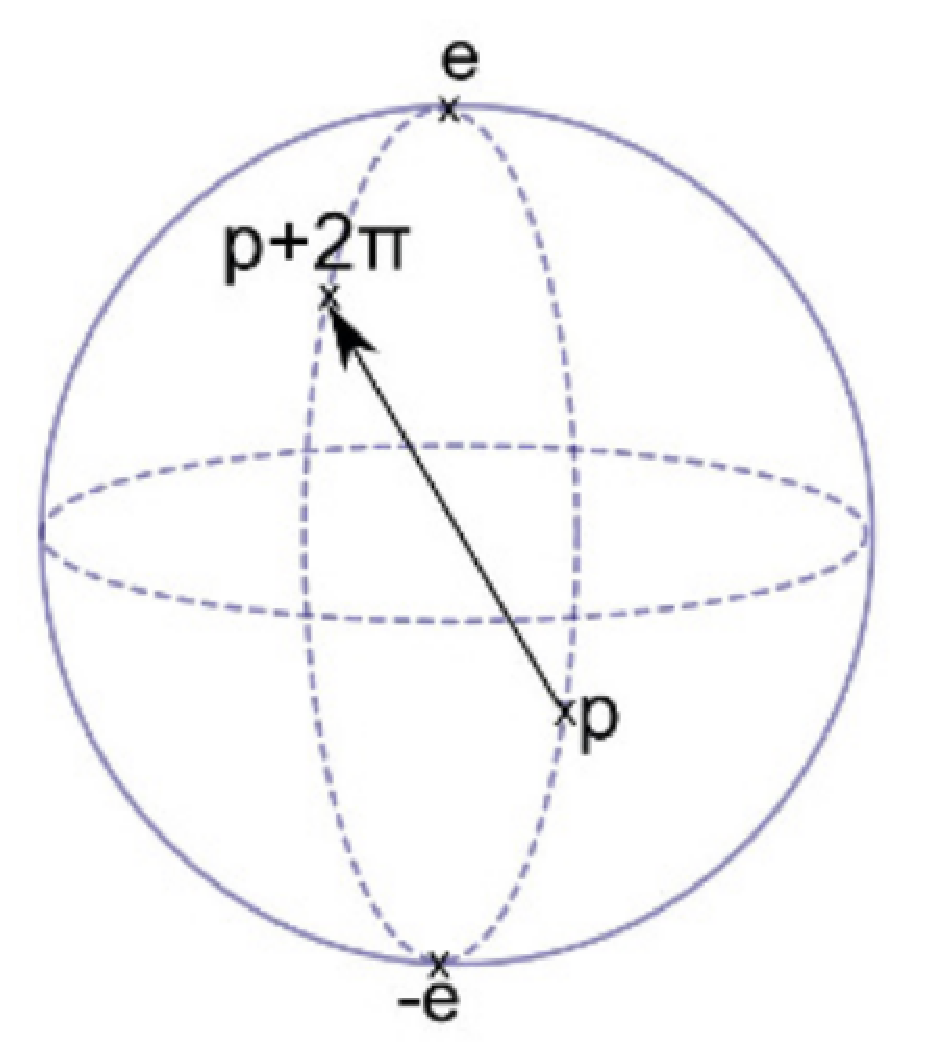
\includegraphics[scale=0.3]{fig3_7.eps} 
		\figcaption{三维超球面$S^3$的一个二维切面($S^3$自身是四维超球的‘表面’,愚蠢的人类没法直接把它画出来),图中可见球面的上半部分对应$\mathcal{SO}(3)$,因为从$\mathcal{SU}(2)$到$\mathcal{SO}(3)$的映射将前者中的$p$点与$p + 2\pi$映射到后者中的同一点。}
	}

因此从流形的角度看,$\mathcal{SU}(2)$群比$\mathcal{SO}(3)$更完整,$\mathcal{SO}(3)$只是其中的一部分。

本书的指导思想之一就是用最基本的群描述大自然最基本的对称性。具体到三维旋转的情况,我们采用$\mathcal{SU}(2)$而非$\mathcal{SO}(3)$。之后其他的对称性我们都这么处理。

世界似乎就是这么设计的!\footnote{先不管设计者有没有、到底是谁吧}比如必须用Poincare群的双覆盖表示来描述基本粒子,而常用却不完整的4-向量表示就不行。要从最深刻的层面描述自然,必须使用覆盖群,而非从覆盖群导出的其他群。

给定一个Lie代数,我们可以通过Lie代数的表示来导出它的覆盖群的表示\mpar{‘表示’的具体含义下一节就讲。},然后把Lie代数元素(生成元)的矩阵表示扔进$\mathrm{e}$指数里面就能得到任意群元的矩阵表示。

这就是Lie理论的威力所在。人类通过纯数学就能揭示自然的某些深刻规律。狭义相对论的标准对称群隐藏了一些真相\mpar{学过量子力学的人可能听说过:标准对称群不能告诉我们自旋!},因为它(尽管常用)不是这一对称性对应的最基本的覆盖群。Poincare群\mpar{简明起见,我们省略了“双覆盖”或“覆盖群”的说法,我们利用Poincare群的一个表示导出相应的Lie代数,然后利用此Lie代数导出相应覆盖群的表示,也就是Poincare双覆盖群的表示。}的覆盖群才是最基本的,我们用它描述自然。

总结一下\mpar{$S^2$未出现,没有与$S^2$对应的Lie群,因为没有三维复数。我们从二维复数$i$直接跳到了四维的四元数$\mathbf{i,j,k}$。}:

\begin{itemize}
	\item $S^1 \hat{=} \mathcal{U}(1) \underbrace{\longleftrightarrow}_{\text{一一对应}} \mathcal{SO}(2)$
	\item $S^3 \hat{=} \mathcal{SU}(2) \underbrace{\longrightarrow}_{\text{二对一}} \mathcal{SO}(3) \hat{=} S^3$的一半
		
		$\Rightarrow \mathcal{SU}(2)$是Lie代数$[J_i, J_j] = i\epsilon_{ijk} J_k$ \, (\ref{equ3.83}\text{式})的覆盖群,因为$S^3$是单连通流形。
\end{itemize}

下一节介绍Lie理论的重要分支 --- 表示论。表示论使我们能够从任意Lie群导出相应基本群。



\section[表示论]{Representation Theory 表示论}
\label{sec3.5}
群论可以描述变换本身而不必联系现实中的特定对象,这是群论的重要特征。

理论上经常从抽象观点来考虑一个群。这意味着用流形结构与群乘法定义群。例如$\mathcal{SU}(2)$就是$S^3$(超球面),群元就是流形中的点,群乘法规定两个群元$a,b$怎样结合,且满足群公理。搞物理的更关心一个群到底能做什么,即{\it 群作用}。

{\bf 同一个}群能作用于{\bf 许多}不同种类的东西\mpar{这话的含义稍后会更加清楚。},这一重要事实使我们定义了{\bf 表示}的概念:群$G$的一个表示就是从$G$到{\it 某个向量空间$V$上全体线性变换组成的集合}\mpar{本书中$V$上的线性变换其实就是指矩阵,即表示$R$把群元映射为矩阵,矩阵通过矩阵乘法作用于向量空间中的向量。}的映射,将表示记作$R$, 映射
\begin{equation}
\label{equ3.86}
R: \underbrace{g}_{\in G} \mapsto R(g)
\end{equation}
其中$R(g)$表示$V$上的某个线性变换。映射$R$必须满足如下条件\mpar{满足这些条件的映射称为{\bf 同态映射},同构映射当然是同态的,并且比同态性还多了一一映射的特征。}:
\begin{itemize}
	\item $R(e) = I$, 恒等元对应的线性变换是恒等变换。
	\item $R(g^{-1}) = \big( R(g) \big)^{-1}$, 逆元对应的变换是逆变换。
	\item $R(g) \circ R(h) = R(g \circ h)$, 群元$g,h$结合对应的变换等于他们分别对应变换的结合。
\end{itemize}

群的表示\mpar{表示的定义可以进行推广,不一定非得是向量空间(别的空间也行)上的线性变换(非线性也可能),拓展后的映射叫{\bf realization}。物理主要考虑向量空间中的线性变换(例如量子力学的Heilbert空间、狭义相对论的Minkowski空间),因此对物理而言表示比更广泛的realization更重要。}将抽象的群元(群流形上的点)与向量空间中的线性变换相联系。尽管按定义来讲,表示是个映射,但大多数情况把表示看做许多矩阵的集合就行了。例如,向量空间\mpar{$\mathbb{R}^3$表示三维Euclidean空间,它的元素就是三维向量,附录A.1里面有很多例子。}$\mathbb{R}^3$中的旋转矩阵组成的集合就是$\mathcal{SO}(3)$群的一个表示,旋转矩阵就是$\mathbb{R}^3$上的线性变换。注意$\mathcal{SO}(3)$群对应的变换也可以作用到其他向量空间。

表示论让我们能系统研究同一个群对不同向量空间的作用,这让群论变得精彩多了。

$\mathcal{SU}(2)$是物理使用最多的群之一。它可以作用到许多向量空间上,比如作用于一维复数向量空间$C^1$,稍后会看到结果是很平凡的。再比如$C^2$,下面我们会详细探究,$C^2$的元素是二维复数向量,因此$\mathcal{SU}(2)$的群元以$2 \times 2$复数矩阵的形式出现,这是$\mathcal{SU}(2)$最常用的表示,之前一直采用此表示。$\mathcal{SU}(2)$还可作用到$C^3$,前人已经对此有完备的研究,$\mathcal{SU}(3)$以$3 \times 3$矩阵出现,作用于$3$维向量。剧透:$\mathcal{SU}(3)$的$C^3$版本的生成元是\mpar{下一节就推倒(无误)它,这里只是为了说明就算是$\mathcal{SU}(\text{`}2\text{'})$\sout{也有不得不守护的东西},也可以作用于三维向量。}:
\begin{equation}
\label{equ3.87}
J_1 = \frac{1}{\sqrt{2}}
	\begin{pmatrix}
		0 & 1 & 0 \\
		1 & 0 & 1 \\
		0 & 1 & 0
	\end{pmatrix}
, \quad
J_2 = \frac{1}{\sqrt{2}}
	\begin{pmatrix}
		0 & -i & 0 \\
		i & 0 & -i \\
		0 & i & 0
	\end{pmatrix}
, \quad
J_3 = \frac{1}{\sqrt{2}}
	\begin{pmatrix}
		1 & 0 & 0 \\
		0 & -1 & 0 \\
		0 & 0 & 0
	\end{pmatrix}
\end{equation}

把生成元扔进$\mathrm{e}$指数里就可得到$\mathcal{SU}(2)$的群元在这个表示之下对应的矩阵的形式。

上面的路可以一直走到$C^n$。因此作者纳闷人们为啥叫把这个群叫$\mathcal{SU}(2)$而非$S^3$。\mpar{在作者撰写本书手稿时就把这个群叫$S^3$,考虑到这个非标准名字会对初学者造成困扰所以改了,因为主流教科书都用$\mathcal{SU}(2)$。}但$\mathcal{SU}(2)$通常定义为满足如下条件的$2 \times 2$(是$2$哟!)复数矩阵集合(即\ref{equ3.33}式)
\begin{equation}
\label{equ3.88}
\mathcal{U}^\dag \mathcal{U} = \mathbf{1}, \quad \det (\mathcal{U}) = 1
\end{equation}
下面会把$\mathcal{SU}(2)$的群元写成$3 \times 3$矩阵的形式,因此要牢记当谈论一般情况$\mathcal{SU}(2)$或其他群群元的时候,我们指的是抽象的群流形中的点,而非只是$2 \times 2$矩阵或者别的。

本章前面都是从群的某个表示出发定义一个群的。比如用$2 \times 2$矩阵定义$\mathcal{SU}(2)$,此方法的优点是群的含义十分具体。在入门之后,把群视为抽象流形的观点\mpar{例如把$\mathcal{SU}(2)$视为$S^3$}更有效,因为这样可以更方便地找出其他有用的群表示。

下面定义几个之后要用的概念,它们与表示的‘等级’有关(不是所有表示都是基本的)。


{\bf 相似变换}。给定任意矩阵$D$与可逆\mpar{矩阵$S$可逆的含义是存在矩阵$T$使得$ST = TS = \mathbf{1}$,$S$的逆矩阵一般记作$S^{-1}$。}矩阵$S$。则可逆变换的形式为:
\begin{equation}
\label{equ3.89}
R \rightarrow R' = S^{-1} RS
\end{equation}

可逆变换与表示的关系在于,给定群$G$,群的表示$R(G)$以及任意可逆矩阵$S$,则$S^{-1} RS$也是群表示。这可以从群的定义直接看出来:$\forall g_1, g_2 \in G$,表示$R$把群元映射为向量空间$V$上的线性变换$R(g_1),R(g_2)$。群的定义要求:
\begin{equation}
\label{equ3.90}
R(g_1) R(g_2) = R(g_1 g_2)
\end{equation}
现在把表示进行相似变换:
\begin{equation}
\label{equ3.91}
S^{-1} R(g_1) \underbrace{SS^{-1}}_{=1} R(g_2) S = S^{-1} R(g_1) R(g_2) S = S^{-1} R(g_1 g_2) S
\end{equation}
上式可得$S^{-1} RS$也是一个表示。如果我们有一个表示,那么就能利用任意可逆矩阵变出好多其他表示,新表示的形式可以更漂亮(比如让它是对角矩阵)。

第二个概念:{\bf 不变子空间}。给定群$G$在向量空间$V$上的表示$R$, 如果$V' \subset V$满足:
\[
\forall v \in V', g \in G, \text{都有} R(g)v \in V'
\]
则$V'$称为$V$的不变子空间\mpar{自然$v \in V$,子空间$V' \subset V$,换言之$V'$的任意元素都是$V$的元素。}。

任意群元作用于$V'$中的任意向量所得向量仍然在$V'$内,这就可以在$V'$上定义群$G$的表示$R'$了:
\begin{equation}
\label{equ3.92}
R'(g) v = R(g) v,\quad \forall v \in V', g \in G
\end{equation}
这种情况下,表示$R$就有一种不太称职的感觉。我们称原来的表示$R$不是原来的向量空间$V$的基本表示,$R$称为子表示。%flag: but a composite of amaller building blocks 未翻译

定义了上述概念之后就能引入超级重要的{\bf 不可约表示}。群$G$在向量空间$V$上的不可约表示$R$意味着除了$0$空间和$V$自身之外再无不变子空间。不可约表示是基本的,它们不能再分解为子表示。从一个不可约表示可导出其他所有表示。

还可以从另一个角度看不可约表示:不可约表示不能通过相似变换变成分块对角矩阵形式。而可约表示能被相似变换变成分块对角形式。表示的可约性很关键,比如描述基本粒子要用不可约表示\mpar{要不用啥呢?},%flag: 边注里的what else没看懂啥意思。。。
基本粒子在变换下的行为由相应对称群的不可约表示描述。

一个群有许多表示\mpar{比如我们前面讨论了二维旋转变换的两种方法 --- 单位复数、$2 \times 2$矩阵。它们都是群流形$S^1$的表示。},怎么知道哪个是描述自然的基本表示?Casimir元可以给我们答案。Casimir元(记作$C$)从Lie代数的元素 --- 生成元导出,它的定义是,对任意生成元$X$都有
\begin{equation}
\label{equ3.93}
[C, X] = 0
\end{equation}
著名的Schur引理\mpar{Schur引理是群论的基本结论之一,它在任何一本群论书都有。}告诉我们,给定一个不可约群$R: \mathfrak{g} \rightarrow GL(V)$\footnote{$GL(V)$表示向量空间$V$上所有线性变换组成的集合。},如果某个线性变换$T: V \rightarrow V$(即$T \in GL(V)$)与所有$R(g), \forall g \in G$对易\footnote{即$\forall g \in G, [R(g), T] = 0$。},则$T$必为恒等变换的常数倍。因此Casimir元是群表示的‘常数’,这些‘常数’的值自然地为群表示‘编号’\mpar{具体内容见下一节的例子。}。之后我们就从Casimir元数值最低的不可约表示开始。

群表示的定义与向量空间$V$有关。一个表示就是将抽象群到$V$的线性变换的映射。线性代数告诉我们以任意矩阵的本征向量为基可以张成一个向量空间。任意Lie群的生成元至少有一个可以通过相似变成对角矩阵\mpar{对角生成元的集合称为Cartan子代数,相应的集合元素称为Cartan生成元。它们在量子场论中大放异彩,因为Cartan生成元的本征值可以给基本粒子‘编号’。例如量子色动力学使用$\mathcal{SU}(3)$群,它有两个Cartan生成元。因此色动力学描述的粒子都有两个‘编号’。通常不用数字表示编号,而是用‘色’(红、蓝、绿…)来标注。再比如描述弱相互作用的$\mathcal{SU}(2)$群只有一个Cartan生成元,因此每个粒子只有一个标签 --- Cartan生成元的本征值。},然后这个对角生成元的本征向量就可作为向量空间的基。

下一节导出$\mathcal{SU}(2)$群的不可约表示。研究$\mathcal{SU}(2)$是因为Lorentz群的Lie代数是两份$\mathcal{SU}(2)$的Lie代数。Lorentz群是Poincare群的一部分,本章由浅入深对他们逐一讨论。



%%%%%%%%%%%%%%%%

\section[$\mathcal{SU}$(2)]{$\mathcal{SU}$(2)  特殊幺正群$\mathcal{SU}$(2)}\label{sec3.6}

我们在3.4.3小节中用具体的矩阵形式进行计算得到了$\mathcal{SU}$(2)生成元的Lie括号\mpar{想当年我们就是用这东西抽象地定义了群的Lie代数。具体结果见
\ref{equ3.83}式}。通过这一点便能得到$\mathcal{SU}(2)$群的进一步表示。回到开头我们对$\mathcal{SU}(2)$群的表示,即$2\times 2$ 的幺正矩阵,其行列式的值为1,但这只是一个特例罢了。在进一步处理这个问题之前,我们可以想一想大概能得到什么样的表示。

\subsection{The Finite-dimensional Irreducible Representations
of $\mathcal{SU}$(2) $\mathcal{SU}$(2)群的有限维不可约表示}
\label{sec3.6.1}

为了知道$\mathcal{SU}$(2)群有限维不可约表示的一些东西,我们用在3.4.3小节中出现的算符的线性组合来定义一个新的算符
\mpar{我们总是能让{\bf{一个}}生成元对角化。遵从惯例,我们选$J_3$为对角阵,由此也生出了矢量空间的基矢。此外,人们一般都是按书上的这种方法引入$J_\pm$的。}:
\begin{align}\label{equ3.94}
  J_+=\frac{1}{\sqrt{2}}(J_1+iJ_2) \\
\label{equ3.95}
  J_-=\frac{1}{\sqrt{2}}(J_1-iJ_2)
\end{align}
用\ref{equ3.83}式可以验证新定义的算符满足如下对易关系:
\begin{align}\label{equ3.96}
  [J_3,J_\pm]=\pm J_\pm \\
\label{equ3.70}
   [J_+,J_-]=J_3
\end{align}
若$v$为$J_3$本征矢,本征值为$b$,用新的算符作用在$v$上会得到很有意思的结果:
\begin{eqnarray}\label{equ3.98}
% \nonumber to remove numbering (before each equation)
\nonumber  J_3(J_\pm v) &=& J_3(J_\pm v)+\underbrace{J_\pm J_3 v -J_\pm J_3 v}_{=0} \\
\nonumber               &=& \underbrace{J_\pm J_3 v}_{=J\pm bv} +\underbrace{J_3J_\pm v -J_\pm J_3 v}_{=[J_3,J_\pm]v}\\
                        &\underbrace{=}_{\ref{equ3.96}\text{式}}& (b\pm 1)J_\pm v
\end{eqnarray}
可见$J_\pm v$也是$J_3$的本征矢,本征值为$(b\pm 1)$\mpar{即$J_3 v=bv$,详见附录C.4。},记该本征矢为$w$,则:
\begin{equation}\label{equ3.99}
  J_3 w=(b\pm 1)w \quad \text{以及} \quad w=J_\pm v
\end{equation}

算符$J_-$和$J_+$通常称为降算符和升算符,也称{\bf{阶梯算符(ladder operators)}}。我们可以通过重复利用阶梯算符$J_\pm$来得到关于$J_3$的本征矢,但这个过程不能无休止地进行,因为不同本征值的本征矢之间是线性独立的,而我们处理的是有限维的表示。这意味着相应的矢量空间是有限维的,我们只能得到有限个独立的矢量。

%此处书上的符号比较混乱,译者对此进行了调整
我们推断一定有一本征矢对应着最大的本征值{\sout{$v_{max}$}}。 若将$J_+$作用到$v$ \  N次以后,得到本征值最大的本征矢$v_{max}$
\begin{equation}\label{equ3.100}
  v_{max}=J_+^N v
\end{equation}
我们有
\begin{equation}\label{equ3.101}
  J_+v_{max}=0
\end{equation}
因为$v_{max}$已经是有最大本征值的本征矢了。称最大本征值为$j:=b+N$。相应有对应着最小本征值的本征矢$v_{min}$,满足
\begin{equation}\label{equ3.102}
  J_-v_{min}=0
\end{equation}
将$J_-$作用到$v_{\color{red}max}$\ M次以后,得到本征值最小的本征矢$v_{min}$
\begin{equation}\label{equ3.103}
  v_{min}=J_-^M v_{max}
\end{equation}
因此,$v_{min}$对应的本征值为$j-M$。为进一步讨论,我们需要知道$J_\pm$作用到本征矢上的具体形式。上述的计算说明,$J_- v_k$应等于$v_{k-1}$乘上一常数:
\begin{equation}\label{equ3.104}
  J_- v_k=\alpha_k v_{k-1}
\end{equation}
如果非要深究$J_-$作用到$v_{max}$上的细节的话,那我只能告诉你
\mpar{见Matthew Robinson. Symmetry and the Standard Model. 第90页,Springer, 1st edition, August
2011. ISBN 978-1-4419-8267-4.} $\alpha$满足
\begin{equation}\label{equ3.105}
  \alpha_{j-k}=\frac{1}{\sqrt{2}}\sqrt{(2j-k)(k+1)}
\end{equation}
注意到当$k=2j$时$\alpha$为0,因此,经过$2j$步之后,我们从梯子的顶端到达了底端。$v_{min}$的本征值即是$j-2j=-j$。 总的来说,我们得到了$2j+1$个本征态的本征值
\begin{equation}\label{equ3.106}
  {-j,-j+1,\dots,j-1,j}
\end{equation}
此式仅当$j$为整数或半整数\mpar{不信的话你就用分数试试看!}时成立。因为我们有$2j+1$个线性独立的本征矢,故矢量空间应为$2j+1$维
\mpar{见此书 189页: Nadir
Jeevanjee. An Introduction to Tensors and
Group Theory for Physicists. Birkhaeuser,
1st edition, August 2011. ISBN 978-
0817647148}。{\it{这些$J_3$的本征矢构成了完备的矢量空间,因为$J_1$和$J_2$ 能够被$J_+$和$J_-$线性表示,就算是一个任意的线性组合$\sum_i a_i v_i$也能变换成另一种线性组合$\sum_i b_i v_i$,其中$a_i ,b_i$是常数。因此,$J_3$ 的本征矢构成了$V$的一个非平庸不变子空间,而我们也在寻找能构成完备矢量空间$V$的不可约表示}}。

我们可以利用上面定义的$2j+1$维的矢量空间及$J_3$的本征矢$v_k$来给出$\mathcal{SU}$(2)的一个表示。进一步说,我们能证明$\mathcal{SU}$(2)的每一种不可约表示都等价于这一种\mpar{例如此书 190页: Nadir
Jeevanjee. An Introduction to Tensors and
Group Theory for Physicists. Birkhaeuser,
1st edition, August 2011. ISBN 978-
0817647148}。

\subsection[$\mathcal{SU}$(2)的 Casimir算符]{The Casimir Operator of $\mathcal{SU}$(2)  $\mathcal{SU}$(2) 的 Casimir算符}
\label{sec3.6.2}
如3.5节所述,我们可以用Casimir算符来标记不同的群表示。$\mathcal{SU}$(2)恰好有一个Casimir算符\mpar{回想一下,Casimir算符指的是那些与群中每个生成元都对易的群元,即$[C,X]=0$。}:
\begin{equation}\label{equ3.107}
  J^2:=(J_1)^2+(J_2)^2+(J_3)^2
\end{equation}
满足定义的条件:
\begin{equation}\label{equ3.108}
  [J^2,J_i]=0
\end{equation}
我们可以用\ref{equ3.95}式和\ref{equ3.94}式定义的$J_\pm$ 来重新表示$J^2$:
\begin{eqnarray}
% \nonumber to remove numbering (before each equation)
\nonumber  J^2 &=&J_+J_- + J_-J_+ +(J_3)^2\\
\nonumber      &=& \frac{1}{2}(J_1+iJ_2)(J_1-iJ_2)+\frac{1}{2}(J_1-iJ_2)(J_1+iJ_2)+(J_3)^2   \\
\nonumber      &=& \frac{1}{2}((J_1)^2-iJ_1J_2+iJ_2J_1+(J_2)^2)+\frac{1}{2}((J_1)^2+iJ_1J_2-iJ_2J_1+(J_2)^2)\\
\nonumber      &&+(J_3)^2 \\
\label{equ3.109}
               &=& (J_1)^2+(J_2)^2+(J_3)^2
\end{eqnarray}
带入\mpar{这些东西只是一些归一化常数,如果我们将$J_\pm$作用到归一态上,得到的结果一般都不是归一化的。然而,学物理的都喜欢用归一态,详细的原因以后再谈。这些常数的推导有些无聊,大体思路是先假设c是个归一化常数, 然后从$J_\pm v_k= c v_{k\pm 1}$开始。计算过程能在大多数的量子力学教材中找到(讲角动量和角动量算符那块儿)。如果你不知道也没关系,因为这节讲的对接下来要讲的东西不是太重要。}
\begin{equation}\label{equ3.110}
  J_+v_k=\frac{1}{\sqrt{2}}\sqrt{(j+k+1)(j-k)} v_{k+1}
\end{equation}
以及
\begin{equation}\label{equ3.111}
  J_-v_k=\frac{1}{\sqrt{2}}\sqrt{(j+k)(j-k+1)} v_{k-1}
\end{equation}
我们就能计算对于每个表示都成立的系数:
\begin{eqnarray}
% \nonumber to remove numbering (before each equation)
  \nonumber  J^2 v_k&=&(J_+J_- + J_-J_+ +(J_3)^2)v_k \\
  \nonumber         &=&J_+J_-v_k + J_-J_+v_k +(J_3)^2v_k \\
  \nonumber         &=& J_+ \frac{1}{\sqrt{2}}\sqrt{(j+k)(j-k+1)} v_{k-1}+J_-\frac{1}{\sqrt{2}}\sqrt{(j+k+1)(j-k)} v_{k+1} +k^2v_k  \\
  \nonumber         &=& \frac{1}{\sqrt{2}}\sqrt{(j+k)(j-k+1)} J_+v_{k-1}+\frac{1}{\sqrt{2}}\sqrt{(j+k+1)(j-k)}J_- v_{k+1} +k^2v_k  \\
  \nonumber         &=& \frac{1}{\sqrt{2}}\sqrt{(j+k)(j-k+1)}   \frac{1}{\sqrt{2}}  \sqrt{(j+(k-1)+1)(j-(k-1))}v_{k}   \\
  \nonumber          && +\frac{1}{\sqrt{2}}\sqrt{(j+k+1)(j-k)} \frac{1}{\sqrt{2}} \sqrt{(j+(k+1))(j-(k+1)+1)} v_{k} +k^2v_k  \\
   \nonumber        &=&\frac{1}{2}(j+k)(j-k+1)v_k +\frac{1}{2}(j-k)(j+k+1)v_k+k^2v_k\\
\label{equ3.112}
                    &=&(j^2+j)v_k=j(j+1)v_k
\end{eqnarray}
现在会看这种表示下的几个特例,当然,从最简单的低维数情况开始。

\subsection[$\mathcal{SU}$(2)的一维表示]{The Representation of $\mathcal{SU}$(2) in one Dimension $\mathcal{SU}$(2)的一维表示}
\label{sec3.6.3}
$j$的最小可能值为0,这样群的表示是一$\,2j+1=2 \cdot 0+1=1$ 维矢量空间。可以看出这个表示是平庸的,因为只有$1 \times 1$矩阵满足$\mathcal{SU}$(2)李代数的对易关系$[J_l,J_m]=i\varepsilon_{lmn} J_n=0$。而生成元0的指数映射得到的是变换$\mathcal{U}=e^0=1$,即群的恒等元。

\subsection[$\mathcal{SU}$(2)的二维表示]{The Representation of $\mathcal{SU}$(2) in two Dimension $\mathcal{SU}$(2)的二维表示}
\label{sec3.6.4}
接下来我们讨论$j=\frac{1}{2}$的情况,这个表示是$\,2j+1=2 \cdot \frac{1}{2}+1=2$ 维的。群的生成元$J_3$的本征值为$\frac{1}{2}$和$\frac{1}{2}-1=-\frac{1}{2}$,正如从\ref{equ3.106} 式中所见,因此$J_3$可表示为
\begin{equation}\label{3.113}
  J_3=\frac{1}{2}\left(
                   \begin{array}{cc}
                     1 & 0 \\
                     0 & -1 \\
                   \end{array}
                 \right)
\end{equation}
此处我们选择$J_3$为对角化的生成元\mpar{由于对易关系, $\mathcal{SU}$(2)群仅有一个对角化的生成元。还有就是记住我们可以用相似变换把一个不对角的生成元变成对角的。}。对应其本征值$+\frac{1}{2}$和$-\frac{1}{2}$的本征矢为:
\begin{equation}\label{equ3.114}
  v_\frac{1}{2}=\left(
                  \begin{array}{c}
                    1 \\
                    0 \\
                  \end{array}
                \right)
                \quad \text{以及} \quad
     v_{-\frac{1}{2}}=\left(
                  \begin{array}{c}
                    0\\
                    1\\
                  \end{array}
                \right)
\end{equation}

可以用在这一基矢下的阶梯算符来得到$\mathcal{SU}$(2)另外两个生成元的矩阵形式
\begin{align}\label{equ3.115}
  J_1=\frac{1}{\sqrt{2}}(J_-+J_+) \\
\label{equ3.116}
  J_2=\frac{i}{\sqrt{2}}(J_--J_+)
\end{align}
这一点可以直接从\ref{equ3.95}式和\ref{equ3.94}式关于$J_\pm$的定义的得到。回忆一下,表示空间中的基矢是由$J_3$ 的本征矢给出的,而我们也基矢给出 用$J_1J_2$。换句话说,$J_1J_2$是由它们作用在$J_3$ 的本征矢上的效果来定义的。例如
\begin{equation}\label{equ3.117}
  J_1v_\frac{1}{2}
  =\frac{1}{\sqrt{2}}
  (J_-+J_+)v_\frac{1}{2}
  =\frac{1}{\sqrt{2}}
  (J_-v_\frac{1}{2}
  +\underbrace{J_+v_\frac{1}{2}}_{=0})
  =\frac{1}{\sqrt{2}}J_-v_\frac{1}{2}
  =\frac{1}{2}v_{-\frac{1}{2}}
\end{equation}
式中用到$J_+v_\frac{1}{2}=0$,因为$\frac{1}{2}$是最大的本征值。最后结果的系数$\frac{1}{2}$是从\ref{equ3.105}式得到的。同理可得
\begin{equation}\label{equ3.118}
  J_1 v_{-\frac{1}{2}}=\frac{1}{\sqrt{2}}(J_-+J_+)v_{-\frac{1}{2}}=\frac{1}{2}v_{-\frac{1}{2}}
\end{equation}
而我们之前得到的基矢是$v_\frac{1}{2}=(1,0)^{{T}}$ 和$v_{-\frac{1}{2}}=(0,1)^{{T}}$,因此$J_1$的矩阵为:
\begin{equation}\label{equ3.119}
  J_1=\frac{1}{2}\left(
                   \begin{array}{cc}
                     0 & 1 \\
                     1 & 0 \\
                   \end{array}
                 \right)
\end{equation}
可以验证上式满足我们所说的$J_1$作用到基矢上的效果
\mpar{推导出的\ref{equ3.117}式为$J_1v_\frac{1}{2}=\frac{1}{2}v_{-\frac{1}{2}}$。带入这里具体的矩阵形式可得
$J_1 v_\frac{1}{2}=\frac{1}{2}
\left(
\begin{array}{cc}
0 & 1 \\
1 & 0 \\
\end{array}
\right)
\left(
\begin{array}{c}
      1 \\
      0 \\
\end{array}
\right)
=\frac{1}{2}
\left(
\begin{array}{c}
      0 \\
      1\\
\end{array}
\right)=\frac{1}{2}v_{-\frac{1}{2}} \quad \surd$。}。 同理可得
\begin{equation}\label{equ3.120}
    J_2=\frac{1}{2}\left(
                   \begin{array}{cc}
                     0 & -i \\
                     i & 0 \\
                   \end{array}
                 \right)
\end{equation}
正如我们在这一章开头寻找$\mathcal{SU}(2)$群Lie代数时所发现的一样(\ref{equ3.81}式),这些生成元$J_i=\frac{1}{2}\sigma_i$正是Pauli 矩阵。可以看出,现在使用表示的是二维表示。当然除此之外还有其他的表示形式,例如我们下节会看到的三维空间中的表示\mpar{再次说明,$\mathcal{SU}(2)$最开始的定义是全体行列式值为1的$2\times 2$幺正矩阵的集合,而在这儿我们采用抽象的定义,即其对应的流形$S^3$,接下来还要讨论这个群的更高维表示,比如$3\times 3$ 矩阵的表示。其实叫成别的名字可能更合适(比如说对应的流形$S^3$),但按照传统,它就叫$\mathcal{SU}(2)$.}。
\subsection[$\mathcal{SU}$(2)的三维表示]{The Representation of $\mathcal{SU}$(2) in two Dimension $\mathcal{SU}$(2)的三维表示}
\label{equ3.6.5}
重复与二维情况相似的操作\mpar{仍然是从对角化的生成元$J_3$出发。{\sout{学过的人都知道}}$J_3$的本征值为(1,0,-1),因此立刻就能得到其矩阵形式。对于$J_1J_2$而言,仍然是从其作用结果出发,即把他们写成$J_\pm$的线性组合然后作用到$J_3$的本征矢上。} 可以得到:
\begin{equation}\label{equ3.121}
J_1=\frac{1}{\sqrt{2}}\left(
\begin{array}{ccc}
0& 1 & 0 \\
1 & 0 & 1 \\
0 & 1 & 0 \\
  \end{array}
\right)
J_2=\frac{1}{\sqrt{2}}\left(
\begin{array}{ccc}
0& -i & 0 \\
i & 0 & -i \\
0 & i & 0 \\
\end{array}
\right)
J_3=\frac{1}{\sqrt{2}}\left(
\begin{array}{ccc}
1& 0 & 0 \\
0 & -1 & 0 \\
0 & 0 & 0 \\
\end{array}
\right)
\end{equation}
这就是$\mathcal{SU}(2)$的三维表示。如果你有兴趣的话,还可以推出三维表示下$\mathcal{SU}(2)$群元的形式(把生成元扔进$\mathrm{e}$指数里。)。介于现在所学已足够理解最重要的Lorentz 群的表示,我们将不会推导更高维的$\mathcal{SU}(2)$表示。
%%%%%%%%%%%%%%%



\section[Lorentz群]{The Lorentz Group $\mathcal{O}(1, 3)$ \quad Lorentz群$\mathcal{O}(1, 3)$}
\label{sec3.7}

\begin{quote}
抽象总是从具体的现实中产生的$\dots$ 你总得从某件事物出发,最后才能把所有现实的痕迹抹除掉。
\end{quote}

\begin{flushright}
{\bf  --- Pablo Picasso}\mpar{引自 Robert S. Root-Bernstein and Michele M. Root-Bernstein. Sparks of Genius. Mariner Books, 1st edition, 8\, 2001. ISBN 9780618127450}
\end{flushright}

本节从Lorentz群{\bf 一种}常用的表示出发导出相应的Lie代数。推导过程与之前$\mathcal{SU}(2)$的情形相同 --- 用$\mathcal{SU}(2)$的$2 \times 2$矩阵表示导出了Lie代数。我们会发现Lorentz群的Lie代数可以用两份$\mathcal{SU}(2)$\ Lie代数表示,这会导出Lorentz群的更多表示。著名的向量表示 --- 即Lorentz群群元为$4 \times 4$矩阵,作用于$4$维向量 --- 仅仅是众多表示中的{\bf 一种}。新表示能描述向量表示不能描述的物理系统。这就是Lie理论的威力所在,它使我们找出对称性隐藏的抽象结构,从而可以描述自然最基本的层面。

首先导出Lorentz群及其子群的特性。Lorentz群定义为Minkowski空间中{\it 所有保证内积不变的变换}组成的集合\mpar{下式的推导在第2章。重复一下,Lorentz群的定义借鉴了Euclidean空间中旋转、反射变换保证Euclidean空间中内积不变的特性。}:
\begin{equation}
\label{equ3.122}
x^\mu x_\mu = x^\mu \eta_{\mu \nu} x^\nu = (x^0)^2 - (x^1)^2 - (x^2)^2 - (x^3)^2
\end{equation}
其中$\eta_{\mu \nu}$表示Minkowski度规:
\begin{equation}
\label{equ3.123}
\eta_{\mu \nu} =
	\begin{pmatrix}
		1 & 0 & 0 & 0 \\
		0 & -1 & 0 & 0 \\
		0 & 0 & -1 & 0 \\
		0 & 0 & 0 & -1
	\end{pmatrix}
\end{equation}

这个定义的条件对变换(矩阵)有什么限制?Lorentz群的群元 --- Lorentz变换通常记作$\Lambda$,考虑变换$x^\mu \rightarrow x'^\mu = \Lambda^\mu_\nu x^\nu$,变换前后的内积为:
\begin{equation}
\label{equ3.124}
x^\mu \eta_{\mu \nu} x^\nu \rightarrow x'^\sigma \eta_{\sigma \rho} x'^\rho = (x^\mu \Lambda^\sigma_\mu) \eta_{\sigma \rho} (\Lambda^\rho_\nu x^\nu) \stackrel{!}{=} x^\mu \eta_{\mu \nu} x^\nu
\end{equation}
由$x^{\mu}$的任意性可得:
\begin{equation}
\label{equ3.125}
\Lambda^\sigma_\mu \eta_{\sigma \rho} \Lambda^\rho_\nu \stackrel{!}{=} \eta_{\mu \nu}
\end{equation}
上式写成矩阵形式\mpar{复习:两个向量的内积用矩阵乘法表示是,左侧的向量转置成行矩阵。因此下式左侧有$\Lambda^T$。}:
\begin{equation}
\label{equ3.126}
\Lambda^T \eta \Lambda \stackrel{!}{=} \eta
\end{equation}
{\bf 上式就是Lorentz变换$\Lambda$定义的数学形式!} 对上式取行列式,利用$\det(AB) = \det(A) \det(B)$可得:
\begin{align}
\label{equ3.127}
\det(\Lambda) \underbrace{\det(\eta)}_{= -1} \det(\Lambda) = \underbrace{\det(\eta)}_{= -1} \rightarrow \det(\Lambda)^2 \stackrel{!}{=} 1 \\
\label{equ3.128}
\rightarrow \det(\Lambda) \stackrel{!}{=} \pm 1
\end{align}

取\ref{equ3.125}式的$\mu = \nu = 0$分量\mpar{稍后就会看到这有什么用。}:
\begin{align}
	\Lambda_0^\sigma \eta_{\sigma \rho} \Lambda_0^\rho \stackrel{!}{=} \underbrace{\eta_{00}}_{=1} \nonumber \\
	\label{equ3.129}
	\rightarrow \Lambda_0^\sigma \eta_{\sigma \rho} \Lambda_0^\rho = (\Lambda_0^0)^2 - \sum_i (\Lambda_0^i)^2 \stackrel{!}{=} 1
\end{align}
由此可得:
\begin{equation}
	\label{equ3.130}
	\Lambda_0^0 \stackrel{!}{=} \pm \sqrt{1 + \sum_i (\Lambda_0^i)^2}
\end{equation}

根据\ref{equ3.128}与\ref{equ3.130}式的正负可以把Lorentz群分成4分支。保证坐标系取向\mpar{这意味着右手坐标系在变换后仍为右手系,左手坐标系在变换后仍为左手系。左手、右手坐标系的定义见附录A.5.}不变的两个分支满足$\det (\Lambda) = +1$. 如果想保证时间轴的方向不变,则需要条件$\Lambda_0^0 \geq 0$,因为
\begin{equation}
	\label{equ3.131}
	x^0 = t \rightarrow x'^0 = t' = \Lambda_\nu^0 x^\nu = \Lambda_0^0 t + \Lambda_1^0 x^1 + \Lambda_2^0 x^2 + \Lambda_3^0 x^3
\end{equation}
如果$\Lambda_0^0 \geq 0$, 则$t'$与$t$同号。

满足$\det(\Lambda) \geq 0$与$\Lambda_0^0 \geq 0$的分支称为$\mathcal{SO}(1, 3)^{\uparrow}$。我们主要研究这个子群,它有漂亮的名字 --- 正规\mpar{‘正规’(proper)意思是$\mathcal{SO}(1, 3)^{\uparrow}$子群的群元都是保证坐标系取向和宇称不变的变换。}或正时\mpar{‘正时’(orthochronous)是指子群的群元保持时间轴的方向不变。}Lorentz群。Lorentz群的这四分支是分离的,因为从一个分支出发,仅用该分支的Lorentz变换无法得到其他任何分支的元素。但引入两个新变换之后就可以从$\mathcal{SO}(1, 3)^\uparrow$出发得到其他分支\mpar{在现在的群表示下这两个算符的矩阵长这样。后面换用不同的表示,它们会大不一样。}:
\begin{align}
	\label{equ3.132}
	\Lambda_P = 
		\begin{pmatrix}
			1 & 0 & 0 & 0 \\
			0 & -1 & 0 & 0 \\
			0 & 0 & -1 & 0 \\
			0 & 0 & 0 & -1
		\end{pmatrix}
\\
	\label{equ3.133}
	\Lambda_T = 
		\begin{pmatrix}
			-1 & 0 & 0 & 0 \\
			0 & 1 & 0 & 0 \\
			0 & 0 & 1 & 0 \\
			0 & 0 & 0 & 1
		\end{pmatrix}
\end{align}
$\Lambda_P$称为宇称算符,相应的宇称变换其实就是镜面反射。$\Lambda_T$称为时间反演算符。

于是完整的Lorentz群$\mathcal{O}(1, 3)$可以表示为如下集合:
\begin{equation}
	\label{equ3.134}
	\mathcal{O}(1, 3) = \{ \mathcal{SO}(1, 3)^\uparrow, \Lambda_P \mathcal{SO}(1, 3)^\uparrow, \Lambda_T \mathcal{SO}(1, 3)^\uparrow, \Lambda_P \Lambda_T \mathcal{SO}(1, 3)^\uparrow \}
\end{equation}

这样,研究Lorentz群的表示就可简化为研究$\mathcal{SO}(1, 3)^\uparrow$的表示,因为只要再找出$\Lambda_P$、$\Lambda_T$的表示,Lorentz群的其他分支就都有啦。

\subsection[Lorentz群的$1$表示]{One Representation of the Lorentz Group \quad Lorentz群的$1$表示}
\label{sec3.7.1}
下面利用Lorentz群的定义(\ref{equ3.125}式)构造Lorentz变换的显式矩阵表示。首先考虑矩阵的形式。对Lorentz群,它的群元作用于$4$向量\mpar{通常狭义相对论涉及的向量空间是四维实Minkowski空间$R^{(1, 3)}$。Lorentz群就是定义在这个空间的(Lorentz变换就是保证$4 \times 4$度规不变的变换),因此首先研究群在$R^{(1, 3)}$上的表示。 类似地,$\mathcal{SU}(2)$群起初是用$2 \times 2$复数矩阵表示的,从那里出发可以得到$\mathcal{SU}(2)$好多其他的表示。},因此群元的形式为$4 \times 4$实数矩阵。矩阵元必须是实数,因为Minkowski空间$R^{(1, 3)}$是实数空间。一般的$4 \times 4$实数矩阵有$16$个参数,而Lorentz群的定义规定了$10$个条件\mpar{自行验证$\Lambda^T \eta \Lambda = \eta$对$\Lambda$的限制条件是$10$个。\sout{留做习题}},这样还剩$6$个自由参数。也就是说描述最一般的Lorentz变换需要$6$个参数。因此只要集齐$6$个线性无关的生成元,就可以召唤Lorentz群的Lie代数。这$6$个生成元\sout{$6$个基}构成Lie代数的一组基,即任意生成元可唯一地表示为它们的线性组合。然后就能计算这些基在Lie括号下的运算结果,从而导出Lie代数的抽象定义。

注意三维Euclidean空间中的旋转矩阵(它们只变换空间坐标而不管时间)满足定义\ref{equ3.125}式。这是因为Minkowski度规的空间部分\mpar{空间部分是指分量$\mu = 1, 2, 3$对应的部分。空间部分通常记作$\eta_{ij}$, 人们习惯用拉丁字母(例如$i,j$)表示从$1$到$3$, 而希腊字母(例如$\mu,\nu$)表示从$0$到$3$。}与$3 \times 3$单位矩阵成比例\mpar{$\eta_{11} = \eta_{22} = \eta_{33} = -1, \eta_{ij}=0, \text{若}i \neq j$}。因此对于只涉及空间坐标的变换,由\ref{equ3.125}可得:
\begin{align*}
	-R^T I_{3 \times 3} R = - R^T R \stackrel{!}{=} -I_{3 \times 3} \\
	\rightarrow R^T I_{3 \times 3} R = R^T R \stackrel{!}{=} I_{3 \times 3}
\end{align*}
上式正是$\mathcal{O}(3)$群的定义式。再加上条件
\begin{equation*}
	\det(\Lambda) \stackrel{!}{=} 1
\end{equation*}
就是$\mathcal{SO}(3)$群的定义。只涉及空间坐标的Lorentz变换的形式为:
\begin{equation*}
	\Lambda_{\mathrm{rot}} =
		\begin{pmatrix}
			1 & \\
			  & R_{3 \times 3}
		\end{pmatrix}
\end{equation*}
其中旋转矩阵$R_{3 \times 3}$的形式见\ref{equ3.23}式,相关推导见\ref{sec3.4.1}节。相应的生成元的推导与\ref{sec3.4.1}节相似,结果为:
\begin{equation}
	\label{equ3.135}
	J_i = 
		\begin{pmatrix}
			0 & \\
			  & J_i^{3\mathrm{dim}}
		\end{pmatrix}
	,\quad 
	i = 1, 2, 3.
\end{equation}
比如,由\ref{equ3.65}式可得:
\begin{equation}
	\label{equ3.136}
	J_1 = 
		\begin{pmatrix}
			0 & \\
			  & J_1^{3 \mathrm{dim}}
		\end{pmatrix}
	=
		\begin{pmatrix}
			0 & 0 & 0 & 0 \\
			0 & 0 & 0 & 0 \\
			0 & 0 & 0 & -1 \\
			0 & 0 & 1 & 0
		\end{pmatrix}
\end{equation}

下面包含时空坐标的变换。按Lie理论的套路,考虑无穷小变换\mpar{Kronecker $\delta$符号定义为
\[\delta^\mu_\rho =
\begin{cases}
	1, & \mu = \rho \\
	0, & \mu \neq \rho
\end{cases}
\]
将Kronecker $\delta$符号写成矩阵形式就是恒等矩阵$I$.
}:
\begin{equation}
\label{equ3.137}
\Lambda^\mu_\rho \approx \delta^\mu_\rho + \epsilon K^\mu_\rho
\end{equation}
将上式带入$\Lambda$的定义条件\ref{equ3.125}式:
\begin{align}
	\Lambda^\mu_\rho \eta_{\mu \nu} \Lambda^\nu_\sigma \stackrel{!}{=} \eta_{\rho \sigma} \nonumber \\
	\rightarrow (\delta^\mu_\rho + \epsilon K^\mu_\rho) \eta_{\mu \nu} (\delta^\nu_\sigma + \epsilon K^\nu_\sigma) \stackrel{!}{=} \eta_{\rho \sigma} \nonumber \\
	\rightarrow \cancel{\eta_{\rho \sigma}} + \epsilon K^\mu_\rho \eta_{\mu \sigma} + \epsilon K^\nu_\sigma \eta_{\rho \nu} + \underbrace{\epsilon^2 K^\mu_\rho \eta_{\mu \nu} K^\nu_\sigma}_{\text{略去高阶小量} \epsilon^2 \text{项}} = \cancel{\eta_{\rho \sigma}} \nonumber \\
	\rightarrow K^\mu_\rho \eta_{\mu \sigma} + K^\nu_\sigma \eta_{\rho \nu} = 0
\end{align}
写成矩阵形式\mpar{第一个下标表示行指标,第二个是列指标。不过指标为一上一下的时候会混淆,这时我们把上下标错开表示,比如$K^\mu_\rho \equiv K^\mu_{\ \rho} \rightarrow (K^T)^\mu_{\  \rho} = K_\rho^{\ \mu}$。矩阵乘法的定义是用行乘以列,因此$K^\nu_{\ \sigma} \eta_{\rho \nu} = \eta_{\rho \nu} K^\nu_{\ \sigma}$的含义为,矩阵$\eta$的第$\rho$行乘以$K$的第$\sigma$列,用矩阵表示为$\eta K$。此外,$K^\mu_\rho \eta_{\mu \sigma} = K^\mu_{\ \rho} \eta_{\mu \sigma} = (K^T)_\rho^{\ \mu} \eta_{\mu \sigma}$,为将上式表示为矩阵乘法而引入矩阵$K$的转置,只有这样才能表示为行乘以列的形式:$K^T$的第$\rho$行乘以$\eta$的第$\sigma$列,上式用矩阵表示为$K^T \eta$。用指标记号可以自由移项,比如$K^\mu_\rho$只是矩阵$K$得一个元素,即一个数。 }:
\begin{equation}
	\label{equ3.139}
	K^T \eta = -\eta K
\end{equation}

上面导出了时空变换的生成元$K$需满足的条件。这些生成元生成的变换称为{\bf 推动}。推动的意思是变换到相对于初始坐标系作匀速直线运动的另一坐标系。比如从一个相对于观者静止的坐标系变换到相对于观者匀速直线运动的坐标系。下面考虑\ref{sec2.1}节中的例子:沿$x$轴的推动变换。由于$y' = y, z' = z$,故生成元的形式为:
\begin{equation}
	\label{equ3.140}
	K_x = 
		\begin{pmatrix}
			\underbrace{
				\begin{pmatrix}
					a & b \\
					c & d
				\end{pmatrix}
			}_{\equiv k_x}
			& \\
			&	\begin{pmatrix}
					0 & 0 \\
					0 & 0
				\end{pmatrix}
		\end{pmatrix}
\end{equation}
			
只需要考虑非零的$2 \times 2$矩阵部分就行了,\ref{equ3.139}式简化为:
\[
	\begin{pmatrix}
		a & c \\
		b & d 
	\end{pmatrix}
	\begin{pmatrix}
		-1 & 0 \\
		0 & 1 
	\end{pmatrix}
	= -
	\begin{pmatrix}
		-1 & 0 \\
		0 & 1 
	\end{pmatrix}
	\begin{pmatrix}
		a & b \\
		c & d
	\end{pmatrix}
\]
不难解得\mpar{$\begin{pmatrix}0 & 1 \\ 1 & 0 \end{pmatrix} \begin{pmatrix}-1 & 0 \\ 0 & 1 \end{pmatrix} = \begin{pmatrix} 0 & 1 \\ -1 & 0 \end{pmatrix}$,以及$- \begin{pmatrix} -1 & 0 \\ 0 & 1 \end{pmatrix} \begin{pmatrix} 0 & 1 \\ 1 & 0 \end{pmatrix} = -\begin{pmatrix} 0 & -1 \\ 1 & 0 \end{pmatrix}$.}:
\[
	k_x =
		\begin{pmatrix}
			a & b \\
			c & d
		\end{pmatrix}
	=
		\begin{pmatrix}
			0 & 1 \\
			1 & 0 
		\end{pmatrix}
\]

因此沿$x$轴的推动变换的生成元为:
\begin{equation}
\label{equ3.141}
	K_x = 
		\begin{pmatrix}
			0 & 1 & 0 & 0 \\
			1 & 0 & 0 & 0 \\
			0 & 0 & 0 & 0 \\
			0 & 0 & 0 & 0
		\end{pmatrix}
\end{equation}

同理可以求出沿$y$、$z$轴推动变换的生成元:
\begin{equation}
\label{equ3.142}
	K_y = 
		\begin{pmatrix}
			0 & 0 & 1 & 0 \\
			0 & 0 & 0 & 0 \\
			1 & 0 & 0 & 0 \\
			0 & 0 & 0 & 0
		\end{pmatrix}
	, \quad
	K_z =
		\begin{pmatrix}
			0 & 0 & 0 & 1 \\
			0 & 0 & 0 & 0 \\
			0 & 0 & 0 & 0 \\
			1 & 0 & 0 & 0 
		\end{pmatrix}
\end{equation}

根据Lie理论,把生成元扔进$\mathrm{e}$指数里就能得到有限大小的变换\mpar{生成元$K_x, K_y, K_z$都是厄米的,即$K_i^\dag = K_i$。因此$\mathrm{e}$指数里不加虚数单位$i$,因为加了之后就变成反厄米的了。}:
\[
	\Lambda_x(\phi) = \mathrm{e}^{\phi K_x}
\]
还以$K_x$为例,简明起见,只考虑其中exciting的部分 --- $2 \times 2$矩阵$k_x$(见\ref{equ3.140}式)。将它的指数函数用级数展开式计算,并利用\mpar{不难算出$k_x^2 = \begin{pmatrix} 0 & 1 \\ 1 & 0 \end{pmatrix} \begin{pmatrix} 0 & 1 \\ 1 & 0 \end{pmatrix} = \begin{pmatrix} 1 & 0 \\ 0 & 1 \end{pmatrix}$,然后$k_x^4 = \mathbf{1}$等等等等。对于奇次幂有$k_x^3 = k_x, k_x^5 = k_x, \dots$}$k_x^2 = \mathbf{1}$:
\begin{align}
	\Lambda_x(\phi) &= \mathrm{e}^{\phi k_x} = \sum_{n = 0}^{\infty} \frac{\phi^n k_x^n}{n!} = \sum_{n = 0}^{\infty} \frac{\phi^{2n}}{(2n)!} \underbrace{k_x^{2n}}_{=1} + \sum_{n = 0}^{\infty} \frac{\phi^{2n + 1}}{(2n + 1)!} \underbrace{k_x^{2n + 1}}_{=k_x} \nonumber \\
	&= \left( \sum_{n = 0}^{\infty} \frac{\phi^{2n}}{(2n)!} \right) I + \left( \sum_{n = 0}^{\infty} \frac{\phi^{2n + 1}}{(2n + 1)!} \right) k_x = \cosh(\phi) I + \sinh(\phi) k_x \nonumber \\
	\label{equ3.143}
	&= 
		\begin{pmatrix}
			\cosh(\phi) & 0 \\
			0 & \cosh(\phi) 
		\end{pmatrix}
	+
		\begin{pmatrix}
			0 & \sinh(\phi) \\
			\sinh(\phi) & 0
		\end{pmatrix}
	=
		\begin{pmatrix}
			\cosh(\phi) & \sinh(\phi) \\
			\sinh(\phi) & \cosh(\phi) 
		\end{pmatrix}
\end{align}
计算过程与\ref{sec3.4.1}的内容相似。这里的求和式里没出现$(-1)^n$,因此结果不是$\sin(\phi)$和$\cos (\phi)$,而是双曲正弦$\sinh(\phi)$和双曲余弦$\cosh(\phi)$。沿$x$轴推动变换的完整$4 \times 4$矩阵为:
\begin{equation}
\label{equ3.144}
	\Lambda_x = 
		\begin{pmatrix}
			\cosh(\phi) & \sinh(\phi) & 0 & 0 \\
			\sinh(\phi) & \cosh(\phi) & 0 & 0 \\
			0 & 0 & 1 & 0 \\
			0 & 0 & 0 & 1
		\end{pmatrix}
\end{equation}
同理可导出沿$y, z$轴的推动变换矩阵:
\begin{align}
\label{equ3.145}
	\Lambda_y = 
		\begin{pmatrix}
			\cosh(\phi) & 0 & \sinh(\phi) & 0 \\
			0 & 1 & 0 & 0 \\
			\sinh(\phi) & 0 & \cosh(\phi) & 0 \\
			0 & 0 & 0 & 1
		\end{pmatrix}
	, \\
\label{equ3.146}
	\Lambda_z = 
		\begin{pmatrix}
			\cosh(\phi) & 0 & 0 & \sinh(\phi) \\
			0 & 1 & 0 & 0 \\
			0 & 0 & 1 & 0 \\
			\sinh(\phi) & 0 & 0 & \cosh(\phi)
		\end{pmatrix}
\end{align}
任意的推动变换都可以分解为上述三个变换矩阵的乘积。

\subsection[Lorentz群其他部分的生成元]{Generators of the Other Components of the Lorentz Group \quad Lorentz群其他部分的生成元}
\label{sec3.7.2}
为得到Lorentz群其他部分\mpar{复习:Lorentz群可以分成$\mathcal{O}(1, 3) = \{ \mathcal{SO}(1, 3)^\uparrow, \Lambda_P \mathcal{SO}(1, 3)^\uparrow, $
$\Lambda_T \mathcal{SO}(1, 3)^\uparrow, \Lambda_P \Lambda_T \mathcal{SO}(1, 3)^\uparrow \}$,上一节导出了$\mathcal{SO}(1, 3)^\uparrow$的生成元。}生成元的形式,只需将宇称算符$\Lambda_P$和时间反演算符$\Lambda_T$作用于刚刚导出的生成元$J_i, K_i$上,用矩阵指标记法写为\mpar{对$J, K$变换需要两个$\Lambda_P$, 因为$J, K$都是二维矩阵,一维一个$\Lambda_P$。这就是算符矩阵在坐标变换下的一般形式,喵。}:
\begin{align}
\label{equ3.147}
	(\Lambda_P)_{\alpha'}^\alpha (\Lambda_P)_{\beta'}^\beta (J_i)^{\alpha' \beta'}\ \ \  \mathclap{ \underbrace{\hat{=}}_{\text{变成矩阵形式}} }\ \ \  \Lambda_P J_i (\Lambda_P)^T = J_i \hat{=} (J_i)^{\alpha \beta} \\
\label{equ3.148}
	(\Lambda_P)_{\alpha'}^\alpha (\Lambda_P)_{\beta'}^\beta (K_i)^{\alpha' \beta'}\ \ \ \mathclap{ \underbrace{\hat{=}}_{\text{变成矩阵形式}} } \ \ \ \Lambda_P K_i (\Lambda_P)^T = -K_i \hat{=} -(K_i)^{\alpha \beta}
\end{align}
上两式可以用上节导出的$J, K$显式矩阵形式暴力计算,例如:
\begin{align}
\label{equ3.149}
	J_x &= 
		\begin{pmatrix}
			1 & 0 & 0 & 0 \\
			0 & 0 & 0 & 0 \\
			0 & 0 & 0 & -1 \\
			0 & 0 & 1 & 0
		\end{pmatrix}
	\rightarrow
	J_x' = \Lambda_P J_x (\Lambda_P)^T = J_x 
	\\
	\Lambda_P J_x (\Lambda_P)^T &= 
		\begin{pmatrix}
			1 & 0 & 0 & 0 \\
			0 & -1 & 0 & 0 \\
			0 & 0 & -1 & 0 \\
			0 & 0 & 0 & -1
		\end{pmatrix}
		\begin{pmatrix}
			1 & 0 & 0 & 0 \\
			0 & 0 & 0 & 0 \\
			0 & 0 & 0 & -1 \\
			0 & 0 & 1 & 0
		\end{pmatrix}
		{
		\begin{pmatrix}
			1 & 0 & 0 & 0 \\
			0 & -1 & 0 & 0 \\
			0 & 0 & -1 & 0 \\
			0 & 0 & 0 & -1
		\end{pmatrix}
		}^T 
	\nonumber \\
\label{equ3.150}
	&=
		\begin{pmatrix}
			1 & 0 & 0 & 0 \\
			0 & 0 & 0 & 0 \\
			0 & 0 & 0 & -1 \\
			0 & 0 & 1 & 0
		\end{pmatrix}
\end{align}
同理,
\begin{align}
\label{equ3.151}
	K_x &= 
		\begin{pmatrix}
			0 & 1 & 0 & 0 \\
			1 & 0 & 0 & 0 \\
			0 & 0 & 0 & 0 \\
			0 & 0 & 0 & 0
		\end{pmatrix}
	\rightarrow K'_x = \Lambda_P K_x (\Lambda_P)^T = -K_x
\\
	\Lambda_P K_x (\Lambda_P)^T &= 
		\begin{pmatrix}
			1 & 0 & 0 & 0 \\
			0 & -1 & 0 & 0 \\
			0 & 0 & -1 & 0 \\
			0 & 0 & 0 & -1
		\end{pmatrix}
		\begin{pmatrix}
			0 & 1 & 0 & 0 \\
			1 & 0 & 0 & 0 \\
			0 & 0 & 0 & 0 \\
			0 & 0 & 0 & 0 
		\end{pmatrix}
		{
		\begin{pmatrix}
			1 & 0 & 0 & 0 \\
			0 & -1 & 0 & 0 \\
			0 & 0 & -1 & 0 \\
			0 & 0 & 0 & -1
		\end{pmatrix}
		}^T
\nonumber \\
\label{equ3.152}
	&= -
		\begin{pmatrix}
			0 & 1 & 0 & 0 \\
			1 & 0 & 0 & 0 \\
			0 & 0 & 0 & 0 \\
			0 & 0 & 0 & 0
		\end{pmatrix}
\end{align}

综上,在宇称变换下:
\begin{equation}
\label{equ3.153}
	J_i \underbrace{\longrightarrow}_{\Lambda_P} J_i, \quad K_i \underbrace{\longrightarrow}_{\Lambda_P} -K_i
\end{equation}
它们之后很有用,因为宇称算符在其他表示之下的形式不会像现在的向量表示这样显然。时间反演算符$\Lambda_T$的推导过程相似,由于$\Lambda_T$只变换第一个分量(时间分量),因此只对$K_i$有影响:
\begin{align}
\label{equ3.154}
	(\Lambda_T)_{\alpha'}^\alpha (\Lambda_T)_{\beta'}^\beta (J_i)^{\alpha' \beta'} \ \ \ \mathclap{ \underbrace{\hat{=}}_{\text{变成矩阵形式}} } \ \ \  \Lambda_T J_i (\Lambda_T)^T = J_i \hat{=} (J_i)^{\alpha \beta} \\
\label{equ3.155}
	(\Lambda_T)_{\alpha'}^\alpha (\Lambda_T)_{\beta'}^\beta (K_i)^{\alpha' \beta'} \ \ \ \mathclap{ \underbrace{\hat{=}}_{\text{变成矩阵形式}} } \ \ \ \Lambda_T K_i (\Lambda_T)^T = -K_i \hat{=} -(K_i)^{\alpha \beta}
\end{align}
或者简写为:
\begin{equation}
\label{equ3.156}
	J_i \underbrace{\rightarrow}_{\Lambda_T} J_i, \quad K_i \underbrace{\rightarrow}_{\Lambda_T} -K_i
\end{equation}

\subsection[$\mathcal{O}(1, 3)^\uparrow$群的Lie代数]{The Lie Algebra of the Proper Orthochronous Lorentz Group \quad $\mathcal{O}(1, 3)^\uparrow$群的Lie代数}
\label{equ3.7.3}
利用上节导出的$\mathcal{O}(1, 3)^\uparrow$生成元的矩阵形式\mpar{推动变换的生成元见\ref{equ3.141}式,旋转变换的生成元见\ref{equ3.62}式。}可以直接计算相应的Lie代数\mpar{Levi-Civita符号$\epsilon_{ijk}$的定义见附录B.5.5.}:
\begin{align}
\label{equ3.157}
	[J_i, J_j] &= i \epsilon_{ijk} J_k \\
\label{equ3.158}
	[J_i, K_j] &= i \epsilon_{ijk} K_k \\
\label{equ3.159}
	[K_i, K_j] &= -i \epsilon_{ijk} J_k
\end{align}
其中$J_i$是旋转变换的生成元,$K_i$是推动的生成元。一般形式的Lorentz变换可以表示为:
\begin{equation}
\label{equ3.160}
	\Lambda = \mathrm{e}^{i J \theta + i K \Phi}
\end{equation}
\ref{equ3.158}式表明两种生成元($J_i$与$K_i$)之间不对易。旋转生成元在对易运算下封闭\mpar{在对易运算下封闭意味着对易子$[J_i, J_j] = J_i J_j - J_j J_i$还是一个旋转变换的生成元。\ref{equ3.157}体现了这一点。},而推动生成元则不是这样\mpar{\ref{equ3.159}表明两个推动生成元$K_i, K_j$的对易子并非推动生成元,而是个转动生成元。}。从$J_i, K_i$出发可以定义在对易运算下封闭并且相互对易的新生成元\footnote{注意区分之后式子中的虚数单位$i$与指标$i$,我们对作者采用这样的符号很抱歉。}:
\begin{equation}
\label{equ3.161}
	N_i^\pm \equiv \frac{1}{2} (J_i \pm i K_i)
\end{equation}
不难算出对易关系为:
\begin{align}
\label{equ3.162}
	[N_i^+, N_j^+] &= i \epsilon_{ijk} N_k^+ \\
\label{equ3.163}
	[N_i^-, N_j^-] &= i \epsilon_{ijk} N_k^- \\
\label{equ3.164}
	[N_i^+, N_j^-] &= 0
\end{align}
这正是$\mathcal{SU}(2)$\, Lie代数的形式!我们发现了$\mathcal{SO}(1, 3)^\uparrow$群的Lie代数包含两份$\mathcal{SU}(2)$的Lie代数。

我们搞了个大新闻,因为前面已经构造了$\mathcal{SU}(2)$的所有不可约表示。然而就像$\mathcal{SO}(3)$那样,Lorentz群不是单连通群\mpar{本书不证明这个命题,证明过程很复杂并且与物理关系不大。},Lie理论告诉我们,对于非单连通群,不存在{\it Lie代数的不可约表示}和{\it 群的表示}之间的一一映射\mpar{这话理解起来有点难。前面提过,一个Lie代数{\bf 总}对应一个特殊的群,这个群的特殊之处在于它是单连通的。导出一个Lie代数的不可约表示之后,再将Lie代数的元素(即生成元)扔进$\mathrm{e}$指数里就能得到单连通群(覆盖群)的表示。只有对于单连通群,前面说的一一映射才存在。 }。{\bf 通过推导Lorentz群Lie代数的不可约表示,可以导出Lorentz群的覆盖群的不可约表示},只要把相应的生成元扔进$\mathrm{e}$指数里就行了。这样导出的一部分表示是Lorentz群的表示,还有一些不是。这些额外的表示很有用处,它们可以用来描述某些基本粒子。

{\it 简明起见,我们把之后要推导的Lorentz群Lie代数的表示,或者Lorentz群双覆盖的表示,全部简称为Lorentz群的表示。 }

$\mathcal{SU}(2)$的每一不可约表示都可以用$\mathcal{SU}(2)$的Casimir算符对应的标量$j$来标记。因此Lorentz群覆盖群\mpar{Lorentz群的覆盖群记作$\mathcal{SL}(2, C)$,它是具有单位行列式(行列式为$1$)的$2 \times 2$复数矩阵的集合。$\mathcal{SL}(2, C) \rightarrow \mathcal{SO}(1, 3)$之间的关系与之前讨论的$\mathcal{SU}(2) \rightarrow \mathcal{SO}(3)$之间的关系类似。}的不可约表示可以用两个数$j_1, j_2$(它们都是整数或半整数)来标记。下面依次研究Lorentz群的$(j_1, j_2)$表示,并利用前面导出的$\mathcal{SU}(2)$群的$ j_1,j_2 = 0, \frac{1}{2}, 1, \dots$表示的形式。


Lorentz群的Lie代数可以用$M_{\mu \nu}$表示为更紧凑的形式,$M_{\mu \nu}$的定义为:
\begin{align}
\label{equ3.165}
	J_i &= \frac{1}{2} \epsilon_{ijk} M_{jk} \\
\label{equ3.166}
	K_i &= M_{0i}
\end{align}
这样Lie代数可表示为:
\begin{equation}
\label{equ3.167}
	[M_{\mu \nu}, M_{\rho \sigma}] = i(\eta_{\mu \rho} M_{\nu \sigma} - \eta_{\mu \sigma} M_{\nu \rho} - \eta_{\nu \rho} M_{\mu \sigma} + \sigma_{\nu \sigma} M_{\mu \rho})
\end{equation}
下面从Lorentz群的Lie代数构造不可约表示,さ、いくぞ!

\subsection[$(0, 0)$表示]{The $(0, 0)$ Representation \quad $(0, 0)$表示}
\label{sec3.7.4}
$\mathcal{SU}(2)$的最低阶表示是平凡的,因为Lie代数对应是$1$维的向量空间,因此生成元必须是$1 \times 1$矩阵,满足对易关系的只有平凡的$0$:
\begin{equation}
\label{equ3.168}
	N_i^+ = N_i^- = 0 \rightarrow \mathrm{e}^{N_i^+} = \mathrm{e}^{N_i^-} = \mathrm{e}^0 = 1
\end{equation}
因此Lorentz群的$(0, 0)$表示作用于{\bf 在Lorentz变换下不变的对象。$(0, 0)$}表示又称为Lorentz{\bf 标量表示}。


\subsection[$(\frac{1}{2}, 0)$表示]{The $(\frac{1}{2}, 0)$ Representation \quad $(\frac{1}{2}, 0)$表示}
\label{sec3.7.5}
$(\frac{1}{2}, 0)$表示就是对$\mathcal{SU}(2)$的一份Lie代数$N_i^+$使用$2$维表示\mpar{复习:表示对应的向量空间的维数是$2j + 1$,因此$j=1/2$表示对应$2\frac{1}{2} + 1 = 2$维向量空间。},另一份Lie代数$N_i^-$使用$1$维表示,即$N_i^- = 0$。由$N_i^-$的定义式\ref{equ3.161}可得:
\begin{align}
\label{equ3.169}
	N_i^- = \frac{1}{2} (J_i - i K_i) = 0 \\
\label{equ3.170}
	\rightarrow J_i = i K_i
\end{align}
此外,根据\ref{sec3.6.4}节中导出的$\mathcal{SU}(2)$的$2$维表示的形式:
\begin{equation}
\label{equ3.171}
	N_i^+ = \frac{\sigma_i}{2}
\end{equation}
其中$\sigma_i$表示Pauli矩阵,其定义见\ref{equ3.81}式。

另一方面:
\begin{equation}
\label{equ3.172}
	N_i^+ \ \ \  \mathclap{ \underbrace{=}_{\ref{equ3.161} \text{式}} } \ \ \  \frac{1}{2} (J_i + i K_i) \  \ \ \mathclap{ \underbrace{=}_{\ref{equ3.170} \text{式}} }  \ \ \  \frac{1}{2} (i K_i + i K_i) = i K_i
\end{equation}
比较\ref{equ3.171}与\ref{equ3.172}式可得:
\begin{align}
\label{equ3.173}
	i K_i = \frac{\sigma_i}{2} \rightarrow K_i = \frac{\sigma_i}{2i} = \frac{i \sigma_i}{2i^2} = -\frac{i}{2} \sigma_i \\
\label{equ3.174}
	\ref{equ3.170}\text{式} \rightarrow J_i = i K_i = -\frac{i^2}{2} \sigma_i = \frac{1}{2} \sigma_i
\end{align}
于是在这一表示下,Lorentz旋转变换为:
\begin{equation}
\label{equ3.175}
	R_\theta = \mathrm{e}^{i \vec{\theta} \vec{J}} = \mathrm{e}^{j \vec{\theta} \frac{\vec{\sigma}}{2}}
\end{equation}
Lorentz推动变换为\footnote{原文$B_\theta$在译文中修改为$B_{\phi}$ --- 译者}:
\begin{equation}
\label{equ3.176}
	B_{\vec{\phi}} = \mathrm{e}^{i \vec{\phi} \vec{K}} = \mathrm{e}^{\vec{\phi} \frac{\vec{\sigma}}{2}}
\end{equation}
将生成元扔进$\mathrm{e}$指数函数里,再将$\mathrm{e}$指数函数用级数展开,就可以算出Lorentz群元的表示。例如,绕$x$轴的旋转变换为:
\begin{equation}
\label{equ3.177}
	R_x(\theta) = \mathrm{e}^{i \theta J_1} = \mathrm{e}^{i \theta \frac{1}{2} \sigma_1} = 1 + \frac{i}{2} \theta \sigma_1 + \frac{1}{2!} \left( \frac{i}{2} \theta \sigma_1 \right)^2 + \dots + \frac{1}{n!} \left( \frac{i}{2} \theta \sigma_1 \right)^n + \dots
\end{equation}
将$\sigma_1$的显式形式(\ref{equ3.81}式)代入,并利用$\sigma_1^2 = \mathbf{1}$可得\mpar{具体过程与\ref{sec3.4.1}中的推导十分相似。}:
\begin{align}
	R_x (\theta) &=
		\begin{pmatrix}
			1 & 0 \\
			0 & 1
		\end{pmatrix}
	+ \frac{i}{2} \theta
		\begin{pmatrix}
			0 & 1 \\
			1 & 0
		\end{pmatrix}
	- \frac{1}{2} \left( \frac{\theta}{2} \right)^2
		\begin{pmatrix}
			1 & 0 \\
			0 & 1
		\end{pmatrix}
	+ \dots 
\nonumber \\
\label{equ3.178}
	&=
		\begin{pmatrix}
			\cos \frac{\theta}{2} & i \sin \frac{\theta}{2} \\
			i \sin  \frac{\theta}{2} & \cos  \frac{\theta}{2}
		\end{pmatrix}
\end{align}
关于其他轴的旋转及推动变换可类似地导出。注意Lorentz变换在这儿用$2 \times 2$复矩阵表示,它们当然不是作用在Minkowski空间的(Minkowski空间的元素是$4$维向量)。Lorentz变换在$(\frac{1}{2}, 0)$表示下作用的{\bf $2$分量}\mpar{之后会看到这些二分量对象与{\bf 自旋向上}和{\bf 自旋向下}的状态有关。}对象称为{\bf 左手旋量}\mpar{这个名字在引入右手旋量之后的含义会更清楚。我们会看到宇称变换将左手旋量变换为右手旋量,反之亦然。旋量通常分为左手和右手的,它们的起源与螺旋性有关 --- 螺旋性与手性不完全相同。重复一遍宇称算符的效果:将左手坐标系变换为右手坐标系,反之亦然。左手、右手旋量的名字就是从那儿来的。}:
\begin{equation}
\label{equ3.179}
	\chi_L = 
		\begin{pmatrix}
			(\chi_L)_1 \\
			(\chi_L)_2
		\end{pmatrix}
\end{equation}

旋量在这里指的是$2$分量对象。左手旋量的另一种定义是在Lorentz变换下根据Lorentz群的$(\frac{1}{2}, 0)$表示变换的对象。注意旋量并不只是$2$分量的向量,旋量有很多新的性质。比如$\mathrm{e}$指数中的$\frac{1}{2}$因子,这个因子使得旋量\mpar{旋量的更多性质可见, chapter 3.2 in J. J. Sakurai. Modern Quantum
Mechanics. Addison Wesley, 1st edition, 9 1993. ISBN 9780201539295}在旋转$2\pi$之后不再和原来相同,而多了一个负号。这个性质十分奇特,因为日常遇到的对象在转$2\pi$之后总是和原来一样。

\begin{quote}
	“旋量可以说是Lorentz变换最基本的数学对象。”
\end{quote}

\begin{flushright}
{\bf  ---  A. M. Steane}\mpar{ Andrew M. Steane. An introduction
to spinors. ArXiv e-prints, December 2013}
\end{flushright}

\subsection[$(0, \frac{1}{2})$表示]{The $(0, \frac{1}{2})$ Representation \quad $(0, \frac{1}{2})$表示}
\label{sec3.7.6}
$(0, \frac{1}{2})$表示的构造过程与之前的$(\frac{1}{2}, 0)$相似。这里$N_i^+$采用$1$维表示,即$N_i^+ = 0$,$N_i^-$采用$2$维表示,即$N_i^- = \frac{1}{2} \sigma_i$。容易认为$(0, \frac{1}{2})$表示和$(\frac{1}{2}, 0)$表示差不多,但并非如此!根据$\ref{equ3.161}$式可得:
\begin{align}
\label{equ3.180}
	N_i^+ = \frac{1}{2} (J_i + iK_i) = 0 \\
\label{equ3.181}
	\rightarrow J_i = -iK_i
\end{align}
注意上面的负号。$N_i^-$采用$\mathcal{SU}(2)$的二维表示(在\ref{sec3.6.4}节推导):
\begin{equation}
\label{equ3.182}
	N_i^- = \frac{1}{2} \sigma_i = \frac{1}{2} (J_i - iK_i) \ \ \ \mathclap{ \underbrace{=}_{\ref{equ3.181} \text{式}} } \ \ \ \frac{1}{2} (-iK_i - iK_i) = -iK_i
\end{equation}
可以得到$(0, \frac{1}{2})$表示的生成元为:
\begin{equation}
\label{equ3.183}
	-iK_i = \frac{1}{2} \sigma_i \rightarrow K_i = -\frac{1}{2i} \sigma_i = \frac{i}{2} \sigma_i
\end{equation}
再结合\ref{equ3.181}式:
\begin{equation}
\label{equ3.184}
	J_i = -iK_i = \frac{1}{2} \sigma_i
\end{equation}
于是,在这一表示之下,Lorentz旋转变换为:
\begin{equation}
\label{equ3.185}
	R_\theta = \mathrm{e}^{i \vec{\theta} \vec{J}} = \mathrm{e}^{i \vec{\theta} \frac{\vec{\sigma}}{2}}
\end{equation}
Lorentz推动变换为\footnote{原文$B_\theta$在译文中修改为$B_{\phi}$ --- 译者}:
\begin{equation}
\label{equ3.186}
	B_{\phi} = \mathrm{e}^{i \vec{\phi} \vec{K}} = \mathrm{e}^{-\vec{\phi} \frac{\vec{\sigma}}{2}}
\end{equation}
可见$(0, \frac{1}{2})$表示的旋转变换与$(\frac{1}{2}, 0)$一样,但推动变换的$\mathrm{e}$指数幂差一个负号。我们推测这两个表示作用的对象{\bf 相似但不完全相同}。 Lorentz群的$(0, \frac{1}{2})$表示作用的对象称为{\bf 右手旋量}:
\begin{equation}
\label{equ3.187}
	\chi_R = 
		\begin{pmatrix}
			(\chi_R)^1 \\
			(\chi_R)^2
		\end{pmatrix}
\end{equation}
左手/右手旋量统称为{Weyl 旋量}。


\subsection[Van der Waerden 符号]{Van der Waerden Notation \quad Van der Waerden 符号}
\label{sec3.7.7}
本节引入便于处理旋量的标记法。上面导出了按不同方式变换的两种旋量,如何将它们区分?它们确实不同,但也并非毫无关系。实际上左手旋量(按$(\frac{1}{2}, 0)$表示变换)与右手旋量(按$(0, \frac{1}{2})$表示变换)之间存在联系。引入带点与不带点的指标来表示不同旋量 --- 这一记法以发明者命名,称为Van der Waerden符号。这能清楚地表示何种对象按何种方式变换。Van der Waerden符号的优点在完整的体系建立起来之后会更清楚。

左手旋量$\chi_L$用不带点的下指标表示:
\begin{equation}
\label{equ3.188}
	\chi_L = \chi_a
\end{equation}
右手旋量用带点的上指标:
\begin{equation}
\label{equ3.189}
	\chi_R = \chi^{\dot{a}}
\end{equation}

下面引入“旋量度规”的概念。旋量度规使得右手旋量可以变换为左手旋量,反之亦然。% but not alone as we will see.
旋量度规定义为\mpar{注意下式就是二维Levi-Civita符号,其定义见附录B.5.5.}:
\begin{equation}
\label{equ3.190}
	\epsilon^{ab} =
		\begin{pmatrix}
			0 & 1 \\
			-1 & 0
		\end{pmatrix}
\end{equation}
不难验证它满足上述性质。再定义\mpar{这里对$\chi_L^C$做一简介。上标$C$表示电荷共轭性,\ref{sec3.7.10}节具体说明它的含义。我们看到$\epsilon$的作用结果是把对象的‘标签’翻转 --- 将左手旋量变换为右手旋量。之后会发现$\epsilon$可以翻转所有‘标签’,比如,电荷的正负。}:
\begin{equation}
\label{equ3.191}
	\chi_L^C \equiv \epsilon \chi_L^*
\end{equation}
其中$*$表示取复共轭。下面将考虑$\chi_L^C$怎样在Lorentz变换下变换,并会发现它正如同右手旋量一样变换。右手旋量由它在Lorentz变换下的变换方式所定义,因此认为$\chi_L^C${\bf 正是}一个右手旋量。下面让推动变换作用到$\chi_L^C$,利用:
\begin{align}
\label{equ3.192}
	(-\epsilon)(\epsilon) = \mathbf{1} \\
\label{equ3.193}
	(\epsilon) \sigma_i^* (-\epsilon) = -\sigma_i
\end{align}
上式不难用Pauli矩阵$\sigma_i$的显式形式直接验证。变换过程为\mpar{下面$\vec{\phi} \vec{\sigma} \equiv \sum_i \sigma_i \phi_i \underbrace{=}_{\text{求和约定}} \sigma_i \phi_i$,$\vec{\sigma}$并非表示“向量”,而只是为了方便而采用的缩写。}:
\begin{eqnarray}
	\chi_L^C \rightarrow (\chi')_L^C &=& \epsilon (\chi')_L^* \nonumber \\
	&=& \epsilon (\mathrm{e}^{\frac{\vec{\phi}}{2} \vec{\sigma} } \chi_L)^* \nonumber \nonumber \\
	&=& \epsilon ( \mathrm{e}^{\frac{\vec{\phi}}{2} \vec{\sigma}} \ \ \ \ \ \mathclap{ \underbrace{(-\epsilon) (\epsilon)}_{=1, \text{见}\ref{equ3.192}\text{式}} } \ \ \ \ \ \chi_L )^* \nonumber \nonumber \\
	&=& \ \ \ \ \ \ \ \mathclap{ \underbrace{\epsilon ( \mathrm{e}^{\frac{\vec{\phi}}{2} \vec{\sigma}^*} (-\epsilon) }_{\ref{equ3.193} \text{式} \rightarrow =\mathrm{e}^{ -\frac{\vec{\phi}}{2} \vec{\sigma} }} } \ \ \ \ \ \ \  (\epsilon) \chi_L^* ) \nonumber \\
	&=& \mathrm{e}^{ -\frac{\vec{\phi}}{2} \vec{\sigma} } \underbrace{\epsilon \chi_L^*}_{= \chi_L^C} \nonumber \\
	\label{equ3.194}
	&=& \mathrm{e}^{-\frac{\vec{\phi}}{2} \vec{\sigma}} \chi_L^C
\end{eqnarray}
由此可见$\chi_L^C$按右手旋量的形式变换\mpar{右手旋量在推动变换下的形式见\ref{equ3.186}式:$B_{\phi} = \mathrm{e}^{i \vec{\phi}\vec{K}} = \mathrm{e}^{-\vec{\phi} \frac{\vec{\sigma}}{2}}$。注意它与左手旋量的变换(\ref{equ3.176}式)的不同:$B_{\phi} = \mathrm{e}^{i \vec{\phi} \vec{K}} = \mathrm{e}^{\vec{\phi} \frac{\vec{\sigma}}{2}}$ }。上式第$5$行利用了$\mathrm{e}^{\frac{\vec{\phi}}{2} \vec{\sigma} }$的Taylor级数展开,并对每一项利用了\ref{equ3.193}式。不难验证$\epsilon (\chi_L^*)$在旋转变换下仍与原来的变换方式相同,理应如此,因此$\chi_L$与$\chi_R$在旋转变换形式相同:
\begin{equation}
\label{equ3.195}
	\chi_L^C \rightarrow (\chi')_L^C = \epsilon (\chi')_L^* = \epsilon ( \mathrm{e}^{ \frac{i\vec{\theta}}{2} \vec{\sigma} } \chi)_L^* = \mathrm{e}^{ \frac{i\vec{\theta}}{2} \vec{\sigma} } \epsilon (\chi_L)^*
\end{equation}
还可以验证以下结果:$\epsilon$在任意Lorentz变换下不变;将右手旋量变换为左手旋量需要用$(-\epsilon)$。

仿照狭义相对论中的张量记号,定义“旋量度规”可以升降旋量的指标:
\begin{equation}
\label{equ3.196}
	\epsilon \chi_L \ \ \ \mathclap{ \underbrace{=}_{\text{用指标记号表示}} } \ \ \ \epsilon^{ac} \chi_c = \chi^a
\end{equation}
其中重复的上下标表示求和(即Einstein求和约定)。此外,从上面可知如果想把$\chi_R$变换为$\chi_L$还需要取复共轭:
\begin{equation}
\label{equ3.197}
	\chi_R = \epsilon \chi_L^*
\end{equation}
用Van der Waerden符号,$\epsilon$取复共轭得到的右手旋量用带点的上指标表示:
\begin{equation}
\label{equ3.198}
	\chi_R = \epsilon \chi_L^* = \chi^{\dot{a}}
\end{equation}
再与指标记号相比较,可以发现$\chi_L$的复共轭可以用带点的下指标表示:
\begin{equation}
\label{equ3.199}
	\chi_L^* = \chi_a^* = \chi_{\dot{a}}
\end{equation}
同理,右手旋量$\chi_R$的复共轭可用不带点的上指标表示:
\begin{equation}
\label{equ3.200}
	\chi_R^* = (\chi^{\dot{a}})^* = \chi^a
\end{equation}

下面考虑$\chi_{\dot{a}}$与$\chi^a$在Lorentz变换下如何改变,这非常重要,$\chi_{\dot{a}}$与$\chi^a$可以构造在Lorentz变换下不变的某种旋量的组合形式\mpar{这些旋量构造出的不变量极为重要,因为我们要导出在所有惯性系下都成立的物理定律。这些不变量的重要性之后会不断体现。}。

从左手旋量在Lorentz变换下的行为出发:
\begin{equation}
\label{equ3.201}
	\chi_L = \chi_a \stackrel{\text{Lorentz 变换}}{\longrightarrow} \chi_a' = \Big( \mathrm{e}^{ i\vec{\theta} \frac{\vec{\sigma}}{2} + \vec{\phi} \frac{\vec{\sigma}}{2}  } \Big)^b_a \chi_b
\end{equation}
考虑旋量$\chi_{\dot{a}}$的变换:
\begin{align}
	\chi_L^* = \chi_a^* = \chi_{\dot{a}} \stackrel{\text{Lorentz 变换}}{\longrightarrow} \chi_{\dot{a}}' = (\chi_a')^* &= \bigg( \Big( \mathrm{e}^{ i\vec{\theta} \frac{\vec{\sigma}}{2} + \vec{\phi} \frac{\vec{\sigma}}{2}  } \big)^b_a \Bigg)^* \chi_b^* \nonumber \\
\label{equ3.202}
	&= \bigg( \mathrm{e}^{-i \vec{\theta} \frac{\vec{\sigma}^*}{2} + \vec{\phi} \frac{\vec{\sigma}^*}{2} } \bigg)^{\dot{b}}_{\dot{a}} \chi_{\dot{b}}
\end{align}
类似地,利用右手旋量的变换形式:
\begin{equation}
\label{equ3.203}
	\chi_R \stackrel{\text{Lorentz 变换}}{\longrightarrow} \chi_R' = \chi'^{\dot{a}} = \Big( \mathrm{e}^{ i\vec{\theta} \frac{\vec{\sigma}}{2} } \Big)^{\dot{a}}_{\dot{b}} \chi^{\dot{b}}
\end{equation}
可以导出旋量$\chi^a$的变换:
\begin{align}
	\chi_R^* = (\chi^{\dot{a}})^* = \chi^a \stackrel{\text{Lorentz 变换}}{\longrightarrow} \chi'^a = (\chi'^{\dot{a}})^* &= \bigg( \Big( \mathrm{e}^{ i\vec{\theta} \frac{\vec{\sigma}}{2} - \vec{\phi} \frac{\vec{\sigma}}{2} } \Big)^{\dot{a}}_{\dot{b}} \bigg)^* (\chi^{\dot{b}})^* \nonumber \\
\label{equ3.204}
	&= \bigg( \mathrm{e}^{-i \vec{\theta} \frac{\vec{\sigma}}{2} - \vec{\phi} \frac{\sigma}{2} } \bigg)^{a}_{b} \chi^b
\end{align}
为了组合出神秘的Lorentz不变量,还需要一件事:考虑两个向量标量积的定义:$\vec{a} \cdot \vec{b} = \vec{a}^T \vec{b}$。仿照这个我们在旋量的标量积定义里也引入转置操作。注意上面新旋量变换式的$\mathrm{e}$指数中出现了Pauli矩阵的复共轭$\sigma_i^*$(例如$\mathrm{e}^{ -i \vec{\theta} \frac{\vec{\sigma}^*}{2} }$),再加上转置操作就变成取厄米共轭的形式:$\sigma_i^\dag = (\sigma_i^*)^T$,其中前面已经解释过符号$\dag$(称为dagger)的含义。所有Pauli矩阵的厄米共轭仍是Pauli矩阵自身,即:
\begin{equation}
\label{equ3.205}
	\sigma_i^\dag = (\sigma_i^*)^T = \sigma_i
\end{equation}
这从Pauli矩阵的形式$\ref{equ3.81}$式容易导出。

比较\ref{equ3.201}与\ref{equ3.204}式,再结合\ref{equ3.205}式,可以看出旋量$\chi_a$的转置与旋量$\chi^{a}$分别对应的变换形式正好抵消,这意味着$(\chi^a)^T \chi_a$是Lorentz变换下的不变量(即在Lorentz变换下不变),因为\mpar{附录B.5.5中提到,$\delta_b^c$称为Kronecker符号,它是单位矩阵的指标形式,即$\delta_b^c = \begin{cases} 1, & b = c \\ 0, & b \neq c \end{cases}$}:
\begin{align}
	(\chi^a)^T \chi_a & \stackrel{\text{Lorentz 变换}}{\longrightarrow} \nonumber \\
	(\chi'^a)^T \chi'_a &= \bigg( \Big( \mathrm{e}^{ -i\vec{\theta} \frac{\vec{\sigma}^*}{2} - \vec{\phi} \frac{\vec{\sigma}^*}{2} } \Big)^a_b \chi^b  \bigg)^T \Big( \mathrm{e}^{i\vec{\theta} \frac{\vec{\sigma}}{2} + \vec{\phi}\frac{\vec{\sigma}}{2} }  \Big)^c_a \chi_c \nonumber \\
	&= (\chi^b)^T \Bigg( \exp\bigg( -i\vec{\theta} \frac{(\vec{\sigma}^*)^T}{2} - \vec{\phi} \frac{(\vec{\sigma}^*)^T}{2}  \bigg) \Bigg)^a_b \big(\mathrm{e}^{ i \vec{\theta} \frac{\vec{\sigma}}{2} + \vec{\phi} \frac{\vec{\sigma}}{2} } \big)^c_a \chi_c \nonumber \\
	&\underbrace{=}_{\ref{equ3.205} \text{式}} (\chi^b)^T  \underbrace{ \Big( \mathrm{e}^{-i \vec{\theta} \frac{\vec{\sigma}}{2} - \vec{\phi} \frac{\vec{\sigma}}{2} } \Big)^a_b \Big( \mathrm{e}^{ i\vec{\theta} \frac{\vec{\sigma}}{2} + \vec{\phi} \frac{\vec{\sigma}}{2} } \Big)_a^c }_{= \delta_b^c} \chi_c \nonumber \\
\label{equ3.206}
	&= (\chi^c)^T \chi_c
\end{align}
类似地,将$\chi_{\dot{a}}$与$\chi^{\dot{a}}$适当组合,利用\ref{equ3.202}、\ref{equ3.203}式可以得出另一个不变量$(\chi_{\dot{a}})^T \chi^{\dot{a}}$。但是形如$(\chi^{\dot{a}})^T \hat{=} \chi_R^T \chi_L$的项不是Lorentz变换下的不变量,因为:
\begin{equation}
\label{equ3.207}
	\chi_R^T \chi_L = (\chi^{\dot{a}})^T \chi_a \rightarrow (\chi'^{\dot{a}})^T \chi'_a = \chi^{\dot{b}} \underbrace{ \Big( \mathrm{e}^{i\vec{\theta} \frac{\vec{\sigma}^T}{2} - \vec{\phi} \frac{\vec{\sigma}^T}{2}}  \Big)^{\dot{a}}_{\dot{b}} \big( \mathrm{e}^{ i \vec{\theta} \frac{\vec{\sigma}}{2} + \vec{\phi} \frac{\vec{\sigma}}{2}} \big)^c_a}_{\neq \delta_b^c} \chi_c
\end{equation}
可见这样的左手旋量与右手旋量结合的项{\bf 并非}Lorentz不变量。综上,Lorentz不变量必须是一对同类上下标组合成的量\mpar{即上下标都带点$\ ^{\dot{a}}_{\dot{a}}$或都不带点$\ ^a_a$}。或者,不变量必须是右手旋量的厄米共轭左乘左手旋量:$\chi_R^\dag \chi_L = (\chi_R^*)^T \chi_L \hat{=} (\chi^a)^T \chi_a$,或者左手旋量的厄米共轭左乘右手旋量:$\chi_L^\dag \chi_R = (\chi_L^*)^T \chi_R \hat{=} (\chi_{\dot{a}})^T \chi^{\dot{a}}$。Lorentz不变量是之后推导的自然界的普适定律的关键。

在上述基础上,$\epsilon^{ab}$的名字“旋量度规”就变得合情合理了,因为旋量间的内积(在Lorentz变换下不变,见\ref{equ3.206}式)可以写为:
\begin{equation}
\label{equ3.208}
	\chi_a^T \chi^a \underbrace{=}_{\ref{equ3.196} \text{式}} \chi_a^T \epsilon^{ab} \chi_b
\end{equation}
与第二章Minkowski空间的内积(它是Lorentz变换的不变量)的定义式\ref{equ2.31}相对比:
\begin{equation}
\label{equ3.209}
	x_\mu y^\mu = x_\mu \eta^{\mu \nu} y_\nu
\end{equation}
其中$\eta^{\mu \nu}$是Minkowski度规。 可见旋量度规与四维向量的Minkowski度规地位相同\mpar{为啥上式 --- 四维向量的内积的定义式当中没有转置操作?其实上式既可以看做向量方程也可视为分量方程,符号$x_\mu$既代表向量本身又代表向量的分量,不幸的是这有时会造成混乱,比如现在。将上式看做分量方程,则无需转置,这对旋量内积也一样。然而转置运算不可或缺,为了避免遗忘,我们在旋量内积的定义式中加上上标$\ ^T$表示强调。对于常用的三维向量有更好的符号避免上述混乱:向量自身用$\vec{a}$,向量分量用$a_i$表示。}。

在定义了上述符号之后,不难写出旋量度规的下标形式:
\begin{equation}
\label{equ3.210}
	\epsilon_{ab} = 
		\begin{pmatrix}
			0 & -1 \\
			1 & 0
		\end{pmatrix}
\end{equation}
因为$(-\epsilon)\big(  \mathrm{e}^{i \vec{\theta} \frac{\vec{\sigma}}{2} - \vec{\phi} \frac{\vec{\sigma}}{2}} \big)^b_a \chi_R = \chi_L$。\mpar{读者可自行检验,但这对之后的内容关系不大。} 一般的Lorentz变换(转动+推动)通常用$\Lambda$表示,当$\Lambda$的指标带点,说明它作用于右手旋量,并由此推断相应的具体形式:
\begin{equation}
\label{equ3.211}
\chi_R \rightarrow \chi'_R = \chi'^{\dot{a}} = \Lambda^{\dot{a}}_{\dot{b}} \chi^{\dot{b}} = \big( \mathrm{e}^{i \vec{\theta} \frac{\vec{\sigma}}{2} - \vec{\phi} \frac{\vec{\sigma}}{2}} \big)^{\dot{a}}_{\dot{b}} \chi^{\dot{b}}
\end{equation}
同理,左手旋量情形:
\begin{equation}
\label{equ3.212}
	\chi_L \rightarrow \chi'_L = \chi'_a = \Lambda^b_a \chi_b = \big(  \mathrm{e}^{i \vec{\theta} \frac{\vec{\sigma}}{2} + \vec{\phi} \frac{\vec{\sigma}}{2}} \big)^b_a \chi_b
\end{equation}
这样$(\frac{1}{2}, 0)$与$(0, \frac{1}{2})$表示下的Lorentz变换记作:
\begin{align}
\label{equ3.213}
	\Lambda_{(\frac{1}{2}, 0)} = \big(  \mathrm{e}^{i \vec{\theta} \frac{\vec{\sigma}}{2} + \vec{\phi} \frac{\vec{\sigma}}{2}} \big)^b_a \hat{=} \Lambda^b_a \\
\label{equ3.214}
	\Lambda_{(0, \frac{1}{2})} = \big(  \mathrm{e}^{i \vec{\theta} \frac{\vec{\sigma}}{2} - \vec{\phi} \frac{\vec{\sigma}}{2}} \big)^b_a \hat{=} \Lambda^{\dot{a}}_{\dot{b}}
\end{align}
Van der Waerden符号非常便捷,它有效地体现了$\chi_L$与$\chi_R$之间的联系。左右旋量之间可以互相变换,因此必然需要一套能将它们联系起来的符号体系。

之后考虑下一个不可约表示,有一位故人正在那里久候。

\subsection[$(\frac{1}{2}, \frac{1}{2})$表示]{ The $( \frac{1}{2}, \frac{1}{2})$ Representation \quad $(\frac{1}{2}, \frac{1}{2})$表示}
\label{sec3.7.8}
在$(\frac{1}{2},  \frac{1}{2})$表示之下,两份$\mathcal{SU}(2)$\ Lie代数\mpar{数学上记作$(\frac{1}{2}, \frac{1}{2}) = (\frac{1}{2}, 0) \otimes (0, \frac{1}{2})$.}$N_i^+, N_i^-$都采用$2$维表示。首先考虑此表示下的Lorentz变换作用的对象是什么。两份Lie代数之间无相互作用,因为$N_i^+, N_i^-$是对易的,即$[N_i^+, N_i^-] = 0$。因此作用的对象(记作$v$)在两份Lie代数下各自独立变换。$v$有两个指标$v_a^{\dot{b}}$,每个指标在独立的$\mathcal{SU}(2)$Lie代数下变换。$v_a^{\dot{b}}$即采用了上节介绍的Van der Waerden符号。

$v_a^{\dot{b}}$的每个指标有两个取值($\frac{1}{2}$和$-\frac{1}{2}$),\footnote{似乎指标应该为$1, 2$? --- 译者} 因为每个表示都是$2$维的,$v$共有$4$个分量。因此$v$可表示为$2 \times 2$矩阵,但$v$也可以表示为四维向量,稍后会看到\mpar{在之前的二维旋转中遇到过类似情况,二维旋转操作可以用单位复数作用到向量对应的复数上来表示,在定义了复数与实数矩阵间的映射后,旋转也可以用实矩阵作用于列向量来表示。}。

首先考虑复数矩阵,一个一般的$2 \times 2$复数矩阵有$4$个复数元素,因此有$8$个自由参数。而据前所述我们只需要$4$个自由参数。任意复矩阵$M$可表示为厄米矩阵$H$$(H^\dag = H)$与反厄米矩阵$A$ ($A^\dag = -A$)之和:$M = H + A$。$2 \times 2$厄米矩阵和反厄米矩阵都有$4$个自由参数。此外,下面会证明厄米矩阵经$(\frac{1}{2}, \frac{1}{2})$表示下的Lorentz变换后仍为厄米矩阵,反厄米矩阵也一样。这意味着厄米矩阵与反厄米矩阵分别组成的集合都是不变子空间(见\ref{sec3.5}节),亦即,一般的$2 \times 2$复矩阵上的表示是可约的。综上所述,下面研究$2 \times 2$ 厄米矩阵(组成的向量空间)上的不可约表示。

$2 \times 2$ 厄米矩阵的一组基\mpar{它的含义是任意$2 \times 2$ 厄米矩阵可以唯一地表示为基的线性组合: $a_0 \mathbf{1} + a_i \sigma_i$。}是Pauli矩阵\mpar{定义见\ref{equ3.81}式。}$\sigma_i, i = 1, 2, 3$加上单位矩阵。

首先考虑$v_{a\dot{b}}$,而非$v_a^{\dot{b}}$,这样可以利用\ref{equ3.81}式的Pauli矩阵的显式形式。注意$v_a^{\dot{b}}, v_{a \dot{b}}$之间可用旋量度规$\epsilon^{\dot{bc}}$相互变换,因此容易从$v_a^{\dot{b}}$回到$v_{a \dot{b}}$。

记$\sigma^0 = I_{2 \times 2} = \begin{pmatrix} 1 & 0 \\ 0 & 1 \end{pmatrix}$,\text{有} \footnote{原文下式等号右侧的$v$应为下指标,译文已改正。}
\begin{equation}
\label{equ3.215}
	v_{a\dot{b}} = v_\nu \sigma^\nu_{a\dot{b}} = v_0 \begin{pmatrix} 1 & 0 \\ 0 & 1 \end{pmatrix} + v_1 \begin{pmatrix} 0 & 1 \\ 1 & 0 \end{pmatrix} + v_2 \begin{pmatrix} 0 & -i \\ i & 0 \end{pmatrix} + v_3 \begin{pmatrix} 1 & 0 \\ 0 & -1 \end{pmatrix}
\end{equation}
上面解释过,我们也可以使用\mpar{这仅是基的选取问题,这里借助Pauli矩阵来选取具有我们之前导出的关于向量变换性质的基底。}$v^{\dot{b}}_a = v_\mu \sigma_{a \dot{c}}^\mu \epsilon^{\dot{bc}}$,这样的话选用的基就是$(\tilde{\sigma}^{\dot{b}})^\mu = \sigma_{a \dot{c}}^\mu \epsilon^{\dot{bc}}$。一般的厄米矩阵表示为:
\begin{equation}
\label{equ3.216}
	v_{a\dot{b}} = 
		\begin{pmatrix}
			v_0 + v_3 & v_1 - i v_2 \\
			v_1 + i v_2 & v_0 - v_3 
		\end{pmatrix}
\end{equation}
上节讲过,不同类的指标按不同方式变换,具体来说:带点的下标与不带点的下标变换方式不同。

下面研究$v_{a\dot{b}}$在Lorentz变换下如何表现,利用不带点的下标的变换式\ref{equ3.202}:
\begin{align}
	v \stackrel{\text{Lorentz变换}}{\longrightarrow} v' = v'_{a \dot{b}} &= \Big( \mathrm{e}^{ i \vec{\theta} \frac{ \vec{\sigma} }{2} + \vec{\phi} \frac{\vec{\sigma}}{2} } \Big)^c_a v_{c \dot{d}} \Bigg( \Big( \mathrm{e}^{ -i \vec{\theta} \frac{ \vec{\sigma}^* }{2} + \vec{\phi} \frac{ \vec{\sigma}^* }{2} } \Big)^{\dot{d}}_{\dot{b}} \Bigg)^T \nonumber \\
	&= \Big( \mathrm{e}^{ i \vec{\theta} \frac{ \vec{\sigma} }{2}  + \vec{\phi} \frac{\vec{\sigma}}{2}} \Big)^c_a v_{c \dot{d}} \bigg( \mathrm{e}^{ -i\vec{\theta} \frac{ \vec{\sigma}^\dag }{2} + \vec{\phi} \frac{ \vec{\sigma}^\dag }{2} } \bigg)^{\dot{d}}_{\dot{b}} \nonumber \\
\label{equ3.217}
	& \underbrace{=}_{\sigma^\dag = \sigma} \Big( \mathrm{e}^{ i \vec{\theta} \frac{ \vec{\sigma} }{2}  + \vec{\phi} \frac{\vec{\sigma}}{2}} \Big)^c_a v_{c \dot{d}} \Big(  \mathrm{e}^{ -i\vec{\theta} \frac{ \vec{\sigma} }{2} + \vec{\phi} \frac{ \vec{\sigma} }{2} } \Big)^{\dot{d}}_{\dot{b}} 
\end{align}

前面说过,厄米矩阵经Lorentz变换后仍为厄米的,下面来验证\mpar{反厄米矩阵经Lorentz变换仍为反厄米矩阵的证明过程同理。只要把下面最后一步$v_{c \dot{d}}^\dag = v_{c \dot{d}}$改成$v_{c \dot{d}}^\dag = -v_{c\dot{d}}$.}:
\begin{align}
	\Big( \mathrm{e}^{ i \vec{\theta} \frac{ \vec{\sigma} }{2}  + \vec{\phi} \frac{\vec{\sigma}}{2}}  \Big)^c_a v_{c \dot{d}} \Big( \mathrm{e}^{ -i \vec{\theta} \frac{ \vec{\sigma} }{2}  + \vec{\phi} \frac{\vec{\sigma}}{2}}  \Big)^{\dot{d}}_{\dot{b}} & \rightarrow \Bigg( \Big( \mathrm{e}^{ i \vec{\theta} \frac{ \vec{\sigma} }{2}  + \vec{\phi} \frac{\vec{\sigma}}{2}}  \Big)^c_a v_{c \dot{d}} \Big( \mathrm{e}^{ -i \vec{\theta} \frac{ \vec{\sigma} }{2}  + \vec{\phi} \frac{\vec{\sigma}}{2}}  \Big)^{\dot{d}}_{\dot{b}} \Bigg)^\dag \nonumber \\
	&\underbrace{=}_{(ABC)^\dag = C^\dag B^\dag A^\dag} \bigg(  \Big( \mathrm{e}^{ -i \vec{\theta} \frac{ \vec{\sigma} }{2}  + \vec{\phi} \frac{\vec{\sigma}}{2}}  \Big)^{\dot{d}}_{\dot{b}}   \bigg)^\dag v^\dag_{c \dot{d}} \bigg(  \mathrm{e}^{ i \vec{\theta} \frac{ \vec{\sigma} }{2}  + \vec{\phi} \frac{\vec{\sigma}}{2}}  \Big)^c_a \bigg)^\dag \nonumber \\
	&= \bigg( \mathrm{e}^{ i \vec{\theta} \frac{ \vec{\sigma}^\dag }{2}  + \vec{\phi} \frac{\vec{\sigma}^\dag}{2}} \bigg)^{\dot{d}}_{\dot{b}} v^\dag_{c \dot{d}} \bigg(  \mathrm{e}^{ -i \vec{\theta} \frac{ \vec{\sigma}^\dag }{2}  + \vec{\phi} \frac{\vec{\sigma}^\dag}{2}}\bigg)^c_a \nonumber \\
\label{equ3.218}
	&\underbrace{=}_{\text{若} v^\dag_{c \dot{d}} = v_{c \dot{d}}} \bigg( \mathrm{e}^{ i \vec{\theta} \frac{ \vec{\sigma} }{2}  + \vec{\phi} \frac{\vec{\sigma}}{2}} \bigg)^{\dot{d}}_{\dot{b}} v_{c \dot{d}} \bigg(  \mathrm{e}^{ -i \vec{\theta} \frac{ \vec{\sigma} }{2}  + \vec{\phi} \frac{\vec{\sigma}}{2}}\bigg)^c_a
\end{align}
一般形式变换的计算过程冗长无聊,这里只推导一个特例\mpar{一般过程的推导可见Matthew Robinson. Symmetry and the Standard Model. Springer, 1st edition, August 2011. ISBN 978-1-4419-8267-4, 128页。},考虑将$v$沿$z$轴做推动变换\mpar{沿$z$轴意味着$\vec{\phi} = (0, 0, \phi)^T$。沿$z$轴的推动变换形式最简单,因为只有$\sigma_3$是对角矩阵,其他方向的推动变换的$\mathrm{e}$指数计算较复杂。}:
\begin{align}
    v_{a\dot{b}} \stackrel{\text{沿} z \text{轴推动}}{\longrightarrow} v'^{a\dot{b}} &= \Big(\mathrm{e}^{\phi \frac{\sigma_3}{2}} \Big)^c_a v_{c \dot{d}} \Big( \mathrm{e}^{\phi \frac{\sigma_3}{2}} \Big)^{\dot{d}}_{\dot{b}} \nonumber \\
    &=  \begin{pmatrix}
            \mathrm{e}^{\frac{\phi}{2}} & 0 \\
            0 & \mathrm{e}^{- \frac{\phi}{2}}
        \end{pmatrix}
        \begin{pmatrix}
            v_0 + v_3 & v_1 - iv_2 \\
            v_1 + iv_2 & v_0 - v_3 
        \end{pmatrix}
        \begin{pmatrix}
            \mathrm{e}^{\frac{\phi}{2}} & 0 \\
            0 & \mathrm{e}^{- \frac{\phi}{2}}
        \end{pmatrix}
        \nonumber \\
\label{equ3.219}
    &=  \begin{pmatrix}
            \mathrm{e}^{\phi} (v_0 + v_3) & v_1 - iv_2 \\
            v_1 + iv_2 & \mathrm{e}^{-\phi} (v_0 - v_3)
        \end{pmatrix}
\end{align}
其中利用了$\sigma_3$是对角矩阵\mpar{$\sigma_3 = \begin{pmatrix} 1 & 0 \\ 0 & -1 \end{pmatrix}$}以及对角矩阵$\mathrm{e}$指数的计算公式:$\begin{pmatrix} \mathrm{e}^{A_{11}} & 0 \\ 0 & \mathrm{e}^{A_{22}} \end{pmatrix}$。将变换后的$v'$用一般形式写出,并与\ref{equ3.219}式进行比较:
\begin{equation*}
    v'_{a\dot{b}} =
        \begin{pmatrix}
            v'_0 + v'_3 & v'_1 - iv'_2 \\
            v'_1 + iv'_2 & v'_0 - v'_3
        \end{pmatrix}
    =
        \begin{pmatrix}
            \mathrm{e}^{\phi} (v_0 + v_3) & v_1 - iv_2 \\
            v_1 + iv_2 & \mathrm{e}^{-\phi} (v_0 - v_3)
        \end{pmatrix}
\end{equation*}
比较可得对象$v$的分量在沿$z$轴的推动变换下的形式为\mpar{下式利用了双曲函数的定义,即由$\cosh \phi \equiv \frac{1}{2} (\mathrm{e}^\phi + \mathrm{e}^{-\phi}, \sinh \phi \equiv \frac{1}{2} (\mathrm{e}^{\phi} - \mathrm{e}^{-\phi})$得出$\mathrm{e}^{-\phi} = (\cosh \phi - \sinh \phi), \mathrm{e}^{\phi} = (\cosh \phi + \sinh \phi)$。当然不这么做也可以,不过用双曲函数使得形式更加紧凑。}:
\begin{align*}
    \rightarrow& v'_0 + v'_3 = \mathrm{e}^{\phi} (v_0 + v_3) = ( \cosh \phi + \sinh \phi) (v_0 + v_3) \\
    \rightarrow& v'_0 - v'_3 = \mathrm{e}^{- \phi} (v_0 - v_3) = ( \cosh \phi - \sinh \phi) (v_0 - v_3)
\end{align*}
解得:
\begin{align}
    \rightarrow& v'_0 = \cosh(\phi) v_0 + \sinh(\phi) v_3 \nonumber \\
\label{equ3.220}
    \rightarrow& v'_3 = \sinh(\phi) v_0 + \cosh (\phi) v_3
\end{align}
上面正是四维向量的Lorentz变换式\mpar{见\ref{equ3.146}式。}:
\begin{align}
    \begin{pmatrix}
        v'_0 \\ v'_1 \\ v'_2 \\ v'_3
    \end{pmatrix}
    &=
    \begin{pmatrix}
        \cosh \phi & 0 & 0 & \sinh \phi \\
        0 & 1 & 0 & 0 \\
        0 & 0 & 1 & 0 \\
        \sinh \phi & 0 & 0 & \cosh \phi
    \end{pmatrix}
    \begin{pmatrix}
        v_0 \\ v_1 \\ v_2 \\ v_3
    \end{pmatrix}
    \nonumber \\
\label{equ3.221}
    &=
        \begin{pmatrix}
            \cosh(\phi) v_0 + \sinh (\phi) v_3 \\
            v_1 \\
            v_2 \\
            \sinh(\phi) v_0 + \cosh(\phi) v_3
        \end{pmatrix}
\end{align}
上述结果对任意Lorentz变换都成立,其他情形(如转动)由读者自行计算验证。由此可见$(\frac{1}{2}, \frac{1}{2})$表示{\bf 正是}4向量表示。用向量形式可以简化计算,因为用变换矩阵乘以向量比三个矩阵相乘要简单。人们熟悉的$4$向量其实与更基本的旋量有关,一个$4$向量{\bf 是}二阶旋量,即具有两个分量,根据Lorentz群的$(\frac{1}{2}, \frac{1}{2})$表示变换的量。此外,$4$向量并非描述最基本物理体系的量,它们不够基\ 本,有一些系统它们无法描述。

有人说“旋量是向量的平方根”,这话与“向量是二阶张量\mpar{不妨把二阶张量简单看成一个二阶矩阵$M_{\mu \nu}$}的平方根”相似,一个二阶张量有两个向量指标,一个向量有两个旋量指标。因此Lorentz变换作用的最基本的对象其实是旋量。

前面讲过Lorentz群有四部分。不同部分之间通过宇称算符与时间反演算符联系\mpar{见\ref{equ3.134}式。},因此为了描述所有保证光速不变的变换,还需要考虑宇称和时间反演算符在各个表示下的形式。本书只考虑宇称变换,因为实验表明自然在宇称变换下并不总是对称的(之后的章节讨论),而且下一节有关宇称变换表示的推导也可应用于时间反演变换。

\subsection[旋量和宇称]{Spinors and Parity \quad 旋量和宇称}
\label{sec3.7.9}
上面没有说明为啥$(\frac{1}{2}, 0)$表示变换的对象叫左手旋量,而$(0, \frac{1}{2})$表示变换的对象叫右手旋量。在简要介绍宇称变换之后这一问题就可以解释了。

前面已经导出了Lorentz群的生成元在宇称变换下的表现,见\ref{equ3.153}式,便利起见重写一遍:
\begin{equation}
\label{equ3.222}
    J_i \underbrace{\rightarrow}_{\mathrm{P}} J_i, \quad K_i \underbrace{\rightarrow}_{\mathrm{P}} -K_i
\end{equation}
利用生成元$N_i^\pm$的定义式\ref{equ3.161}式,在此也重写一遍:
\begin{equation}
\label{equ3.223}
    N_i^\pm = \frac{1}{2} (J_i \pm iK_i)
\end{equation}
可见在宇称变换之下$N^+ \leftrightarrow N^-$。因此$(0, \frac{1}{2})$表示下的Lorentz变换经宇称变换之后变成$(\frac{1}{2}, 0)$表示下的变换,反之亦然。这就是左手、右手旋量名字的来历\mpar{常见的名字是left- / right- handed 旋量,但这个名字会引起混乱,因为left-handed、right-handed与螺旋性(helicity)的概念有关,螺旋性与手征性(chirality)是不同的东西。尽管如此这个名字还是反映了在宇称变换下某个“左”的东西变成了“右”的。}。就像右手坐标系在宇称变换下变为左手系那样,Lorentz群的这两个表示也在宇称变换下来回变。

旋转变换在两个表示之下相同,而推动变换差一个负号,上述宇称变换的效果可总结为:
\begin{align}
\label{equ3.224}
    (\Lambda_{\vec{K}})_{(\frac{1}{2}, 0)} = \mathrm{e}^{\vec{\phi} \vec{K}} &\underbrace{\rightarrow}_{\mathrm{P}} \mathrm{e}^{- \vec{\phi} \vec{K}} = (\Lambda_{\vec{K}})_{(0, \frac{1}{2})} \\ 
\label{equ3.225}
    (\Lambda_{\vec{K}})_{(0, \frac{1}{2})} = \mathrm{e}^{- \vec{\phi} \vec{K}} &\underbrace{\rightarrow}_{\mathrm{P}} \mathrm{e}^{\vec{\phi} \vec{K}} = (\Lambda_{\vec{K}})_{(\frac{1}{2}, 0)}
\end{align}
可见,描述一个在宇称变换下不变的物理体系同时需要左手旋量{\bf 和}右手旋量。最简单的做法是把它们上下放置在一个对象中,该对象称为{\bf Dirac旋量}:
\begin{equation}
\label{equ3.226}
    \Psi =
        \begin{pmatrix}
            \chi_L \\ \xi_R
        \end{pmatrix}
    =
        \begin{pmatrix}
            \chi_a \\ \xi^{\dot{a}}
        \end{pmatrix}
\end{equation}
前面提过左手、右手旋量统称{\bf Weyl旋量},我们称一个Dirac旋量$\Psi$包含两个Weyl旋量$\chi_L$和$\xi_R$。注意$\Psi$是一般形式,即$\chi_L$与$\xi_R$之间并未钦点任何关系。而具有如下形式的Dirac旋量
\begin{equation}
\label{equ3.227}
    \Psi_{M} =
        \begin{pmatrix}
            \chi_L \\ \chi_R
        \end{pmatrix}
\end{equation}
就是一个特例,称为Majorana旋量。Dirac旋量或Majorana旋量{\bf 不是四维向量},它们的变换方式截然不同。Dirac旋量按Lorentz群的$(\frac{1}{2}, 0) \oplus (0, \frac{1}{2})$表示\mpar{$(\frac{1}{2}, 0) \oplus (0, \frac{1}{2})$表示是一个{\bf 可约}表示,这从它的变换矩阵是分块对角矩阵可以看出。而四维向量按$(\frac{1}{2}, \frac{1}{2}) = (\frac{1}{2}, 0) \otimes (0, \frac{1}{2})$表示变换。}变换,把左右旋量分别对应的变换矩阵写成一个分块对角的大矩阵就是新的变换矩阵:
\begin{equation}
\label{equ3.228}
    \Psi \stackrel{\text{Lorentz变换}}{\longrightarrow} \Psi' = \Lambda_{(\frac{1}{2}, 0) \oplus (0, \frac{1}{2})} \Psi = 
        \begin{pmatrix}
            \Lambda_{(\frac{1}{2}, 0)} & 0 \\
            0 & \Lambda_{(0, \frac{1}{2})}
        \end{pmatrix}
        \begin{pmatrix}
            \chi_L \\ \xi_R
        \end{pmatrix}
\end{equation}
例如,$\Psi$的推动变换为:
\begin{equation}
\label{equ3.229}
    \Psi \stackrel{\text{推动变换}}{\longrightarrow} \Psi' = 
        \begin{pmatrix}
            \mathrm{e}^{\vec{\phi} \frac{\vec{\sigma}}{2}} & 0 \\
            0 & \mathrm{e}^{-\vec{\phi} \frac{\vec{\sigma}}{2}}
        \end{pmatrix}
        \begin{pmatrix}
            \chi_L \\ \xi_R
        \end{pmatrix}
\end{equation}
Dirac旋量在宇称变换下的行为值得考虑,因为知道这以后就能检验某个理论是否在宇称变换下是不变的。我们知道宇称变换下$N^+ \leftrightarrow N^-$,因此Dirac旋量经宇称变换后不再是Dirac旋量(即那个根据Lorentz群的$(\frac{1}{2}, 0) \oplus (0, \frac{1}{2})$表示变换的对象),再考虑到:
\begin{equation}
\label{equ3.230}
    \left( 0, \frac{1}{2} \right) \underbrace{\leftrightarrow}_{\mathrm{P}} \left( \frac{1}{2}, 0 \right)
\end{equation}
可以断定,因为Dirac旋量按$(\frac{1}{2}, 0) \oplus (0, \frac{1}{2})$表示变换,故变换后的对象按照$ (0, \frac{1}{2}) \oplus (\frac{1}{2}, 0)$表示变换。
\begin{equation}
\label{equ3.231}
    \Psi^P \stackrel{\text{Lorentz变换}}{\longrightarrow} (\Psi^P)' = \Lambda_{ (0, \frac{1}{2}) \oplus (\frac{1}{2}, 0)} \Psi^P = 
        \begin{pmatrix}
            \Lambda_{(0, \frac{1}{2})} & 0 \\
            0 & \Lambda_{(\frac{1}{2}, 0)}
        \end{pmatrix}
        \begin{pmatrix}
            \xi_R \\ \chi_L
        \end{pmatrix}
\end{equation}
因此
\begin{equation}
\label{equ3.232}
    \Psi = 
        \begin{pmatrix}
            \chi_L \\ \xi_R
        \end{pmatrix}
    \stackrel{\text{宇称变换}}{\longrightarrow} 
    \Psi^P = 
        \begin{pmatrix}
            \xi_R \\ \chi_L
        \end{pmatrix}
\end{equation}
宇称变换将Dirac旋量(包含$\xi_R, \chi_L$)变换为另一个同样具有$\xi_R, \chi_L$的对象,只是上下位置变了。宇称变换的效果并非$\xi_L \rightarrow \xi_R$,具有这一效果的变换之后再讲述。

\subsection[旋量与电荷共轭]{Spinors and Charge Conjugation \quad 旋量与电荷共轭}
\label{sec3.7.10}
\ref{sec3.7.7}节遇到了能使左手、右手旋量来回变换的变换(好绕),$\chi_L \rightarrow \chi_L^C = \epsilon \chi_L^* =  \chi_R$, $\xi_R \rightarrow \xi_R^C = (-\epsilon) \xi_R^* = \xi_L$。此变换不属于Lorentz群,下面从另一角度来理解这一变换。

到目前为止这个变换仅仅是升降旋量指标的技巧,现在考虑Dirac旋量在该变换下的表现,不难得到:
\begin{equation}
\label{equ3.233}
    \Psi = 
        \begin{pmatrix}
            \chi_L \\ \xi_R
        \end{pmatrix}
    \rightarrow \tilde{\Psi} = 
        \begin{pmatrix}
            \chi_L^C \\ \xi_R^C
        \end{pmatrix}
    =
        \begin{pmatrix}
            \chi_R \\ \xi_L
        \end{pmatrix}
\end{equation}
不幸的是新生儿$\tilde{\Psi}$的变换方式与Dirac旋量不同\mpar{与之前的宇称变换不同,这里可以选择,我们更喜欢新对象与原来的对象种类相同。$\tilde{\Psi}$可以视为经宇称变换和电荷共轭变换后的Dirac旋量。},Dirac旋量在推动变换下的表现是:
\begin{equation}
\label{equ3.234}
    \Psi \rightarrow \Psi' = 
        \begin{pmatrix}
            \mathrm{e}^{\vec{\theta} \frac{\vec{\sigma}}{2}} & 0 \\
            0 & \mathrm{e}^{-\vec{\theta} \frac{\vec{\sigma}}{2}}
        \end{pmatrix}
        \begin{pmatrix}
            \chi_L \\ \xi_R
        \end{pmatrix}
\end{equation}
$\tilde{\Psi}$按下式变换:
\begin{equation}
\label{equ3.235}
    \tilde{\Psi} \rightarrow \tilde{\Psi}' = 
        \begin{pmatrix}
            \mathrm{e}^{-\vec{\theta} \frac{\vec{\sigma}}{2}} & 0 \\
            0 & \mathrm{e}^{\vec{\theta} \frac{\vec{\sigma}}{2}}
        \end{pmatrix}
        \begin{pmatrix}
            \chi_L \\ \xi_R
        \end{pmatrix}
\end{equation}
它是一种新对象,因为它按照Lorentz群的不同表示进行变换。记作:
\begin{equation}
\label{equ3.236}
    \Psi = 
        \begin{pmatrix}
            \chi_L \\ \xi_R
        \end{pmatrix}
    \rightarrow
    \Psi^C = 
        \begin{pmatrix}
            \xi_R^C \\ \chi_L^C
        \end{pmatrix}
    =
        \begin{pmatrix}
            \xi_L \\ \chi_R
        \end{pmatrix}
\end{equation}
上式的变换是刚才的变换+Dirac旋量的Lorentz变换。这个新变换通常称为{\bf 电荷共轭(charge conjugation)}变换,这个名字有点误导性。由上式可知该变换将左手旋量变为右手旋量,也就是把描述基本粒子的一个标签翻转一下\mpar{选读:注意Weyl旋量实际上是个二分量对象,稍后我们会定义称为‘自旋’的可观测量,它由$\frac{1}{2} \sigma_3$描述。矩阵$\epsilon$可以将自旋算符$\frac{1}{2} \sigma_3$本征值$+\frac{1}{2}$的本征向量变换为本征值$-\frac{1}{2}$对应的本征向量。这称为自旋反转,即一个自旋$\frac{1}{2}$的对象变换为自旋$-\frac{1}{2}$的对象。}。之后会看到该算符不止能翻转这一个标签,而是对基本粒子的所有标签都有效。其中一个标签是电荷,因此该变换称为电荷共轭,在推导如何翻转电荷之前,先要学习电荷到底是啥。有一点是很重要的:不止电荷能翻,别的标签都可以。

我们可以接着推导Lorentz群的更高维表示,但到现在为止所有物理中常用的有限维不可约表示都已导出。物理上还要用到无限维表示,用它来变换物理场。

\subsection[无限维表示]{Infinite-Dimensional Representations \quad 无限维表示}
\label{sec3.7.11}
上面几节讨论了Lorentz群的有限维表示及其分类,这些有限维表示下的群元作用于$1$-, $2$-或$4$-分量的对象。物理中经常处理在时空中动力学演化的对象,下面考虑它们如何变换。前面处理的Lorentz变换可以写成如下形式:
\begin{equation}
\label{equ3.237}
    \Phi_a \rightarrow \Phi'_a = M_{ab}(\Lambda) \Phi_b
\end{equation}
其中$M_{ab} (\Lambda)$是Lorentz变换$\Lambda$在某个有限维表示之下的矩阵形式。例如$M_{ab} (\Lambda)$是个作用于Weyl旋量的$2 \times 2$矩阵,作用的结果无非是新对象的分量为旧对象分量的线性组合。如果$\Phi$分布在四维时空,即\mpar{$\mathbf{x}$是时空坐标$t, x, y, z$的缩写。}$\Phi = \Phi(\mathbf{x})$,则Lorentz变换(除了变换$\Phi$之外)还将变换时空坐标,一般情况下:
\begin{equation}
\label{equ3.238}
    x^\mu \rightarrow \Lambda^\mu_\nu x^\nu
\end{equation}
其中$\Lambda^\mu_\nu$是向量表示(即$(\frac{1}{2}, \frac{1}{2})$表示)下的Lorentz变换。场的Lorentz变换为\mpar{大部分文献采用对称操作的Wigner惯例形式:$\Phi_a (\mathbf{x}) \rightarrow M_{ab} (\Lambda) \Phi_b (\Lambda^{-1} \mathbf{x})$,但我们没有什么理由在这里这么写。}:
\begin{equation}
\label{equ3.239}
    \Phi_a (\mathbf{x})  \rightarrow M_{ab} (\Lambda) \Phi_b (\Lambda \mathbf{x}) 
\end{equation}
上式的变换包含两部分。一部分变换作用于$\Phi_a$,对应于有限维表示;另一部分变换作用于坐标。第二变换作用于无限维\mpar{$\Phi$的每个分量都是坐标$\mathbf{x}$的函数。作用于$\Phi_a (\mathbf{x})$(即时空坐标的函数)The corresponding operators act on $\Phi_a ( \mathbf{x} )$ , i.e. functions of the coordinates and the space of functions is in this context infinite- dimensional. 函数空间之所以是无限维是由于基函数的个数是无穷多的。任意函数用无穷多的基函数展开在附录D.1的Fourier展开中讲述。}向量空间,因此需要用无限维表示。Lorentz群的无限维表示由如下微分算符\mpar{下式的符号$\partial^\nu$ 是偏导数符号$\frac{\partial}{\partial x_\nu}$的简写。}给出:
\begin{equation}
\label{equ3.240}
    M^{\mathrm{inf}}_{\mu \nu} = i (x^\mu \partial^\nu - x^\nu \partial^\mu)
\end{equation}
读者可自行验证$M^{\mathrm{inf}}_{\mu \nu}$满足Lorentz Lie代数\ref{equ3.167}式,并且可以变换坐标。

这样坐标变换的形式为\mpar{$M^{\mu \nu}$在\ref{equ3.165}式定义。分量$\omega_{\mu \nu}$与通常的转动角度$\theta_i$的关系为$\theta_i = \frac{1}{2} \epsilon_{ijk} \omega_{jk}$,与推动参数$\phi_i$的关系为$\phi_i = \omega_{0i}$。}:
\begin{equation}
\label{equ3.241}
    \Phi (\Lambda \mathbf{x}) = \mathrm{e}^{ -i \frac{\omega^{\mu \nu}}{2} M^{\mathrm{inf}}_{\mu \nu} \Phi (\mathbf{x}) }
\end{equation}
其中$\mathrm{e}$指数函数定义为它的级数展开,前面已经讲过。完整的Lorentz变换是有限维表示$M^{\mathrm{fin}}_{\mu \nu}$与无限维表示$M^{\mathrm{inf}}_{\mu \nu}$变换的组合:
\begin{equation}
\label{equ3.242}
    \Phi_a (\mathbf{x}) \stackrel{\mathrm{Lorentz\text{变换}}}{\longrightarrow} \bigg( \mathrm{e}^{ -i \frac{\omega^{\mu \nu}}{2} M^{\mathrm{fin}}_{\mu \nu} }\bigg)^b_a \mathrm{e}^{ -i \frac{\omega^{\mu \nu}}{2} M^{\mathrm{inf}}_{\mu \nu} } \Phi_b (\mathbf{x}) 
\end{equation}
矩阵$M^{\mathrm{fin}}_{\mu \nu}$是有限维的,它可以并入无限维矩阵中:
\begin{equation}
\label{equ3.243}
    \Phi_a (\mathbf{x}) \stackrel{\mathrm{Lorentz\text{变换}}}{\longrightarrow} \bigg( \mathrm{e}^{ -i \frac{\omega^{\mu \nu}}{2} M_{\mu \nu} } \bigg)^b_a \Phi_b (\mathbf{x})
\end{equation}
其中$M_{\mu \nu} = M_{\mu \nu}^{\mathrm{fin}} + M^{\mathrm{inf}}_{\mu \nu}$。上式对应的Lorentz群表示称为{\bf 场表示}。

现在可以讨论{\bf 平移}变换,即时空中某点的对象变换到另一点的变换。平移变换的结果并非各分量的组合,因此不需要有限维表示描述平移,而很容易地找到相应的无限维表示。这不再是Lorentz群的部分,但是自然定律应该在时空各点都相同。Lorentz群(推动+转动)加上平移变换称为Poincare群,下一节具体讲述。这里首先引入平移的无限维表示。简明起见,考虑一维情形,一个函数沿$x$轴的{\bf 无穷小}平移变换为:
\begin{equation*}
    \Phi (x) \rightarrow \Phi (x + \epsilon) = \Phi (x) + \ \ \ \ \ \mathclap{ \underbrace{ \partial_x \Phi (x) }_{\text{沿x轴的‘变化率’}} } \ \ \ \ \  \epsilon
\end{equation*}
上式就是Taylor级数展开的前两项。按照惯例,相应的生成元额外乘以$-i$:
\begin{equation}
\label{equ3.244}
    P_i \equiv -i \partial_i
\end{equation}
这样,任意的有限大小的平移变换为:
\begin{equation*}
    \Phi (x) \rightarrow \Phi (x + a) = \mathrm{e}^{-i a^i P_i} \Phi (x) = \mathrm{e}^{a^i \partial_i} \Phi (x)
\end{equation*}
其中$a^i$表示沿各个方向的平移数量。把$\mathrm{e}$指数函数展开为Taylor级数\mpar{这在附录B.4.1中推导。}就能看出上式就是$\Phi (x + a)$的Taylor展开\mpar{这在附录B.3中推导。}。平移到另一个时间点使用$P_0 = i \partial_0$,平移到另一空间点使用$P_i = -i \partial_i$。

\section[Poincare群]{The Poincare group \quad Poincare群}
\label{sec3.8}
现在考虑自然界完整的时空对称群:Poincare群。Lorentz群包含转动和推动变换,而保证光速不变的还有时空中的平移变换,因为在不同时空点测量的光速是相同的。等价地说,光速与所用坐标系原点的位置无关。将这一对称性加入Lorentz群之后就得到Poincare群\mpar{Poincare群并非Lorentz群与平移变换的直和(direct sum),而是半直和(semi-direct sum),但现在可以忽略此数学细节。}:
\begin{align}
    \text{Poincare群} &= \text{Lorentz群 {\bf +} 平移} \nonumber \\
\label{equ3.245}
    &= \text{旋转 {\bf +} 推动 {\bf +} 平移}
\end{align}
Poincare群的生成元是Lorentz群的生成元$J_i, K_i$加上平移变换的在Minkowski空间的生成元$P_\mu$。

用$J_i, K_i, P_\mu$表示的Lie代数为\mpar{这些不是很有用... 这里列出只是为了完整。}:
\begin{align}
\label{equ3.246}
    [J_i, J_j] &= i \epsilon_{ijk} J_k \\
\label{equ3.247}
    [J_i, K_j] &= i \epsilon_{ijk} K_k \\
\label{equ3.248}
    [K_i, K_j] &= -i \epsilon_{ijk} J_k \\
\label{equ3.249}
    [J_i, P_j] &= i \epsilon_{ijk} P_k \\
\label{equ3.250}
    [J_i, P_0] &= 0 \\
\label{equ3.251}
    [K_i, P_j] &= i \delta_{ij} P_0 \\
\label{equ3.252}
    [K_i, P_0] &= -i P_i
\end{align}
上面的形式比较凌乱,定义$M_{\mu \nu}$来表述会整洁的多,$M_{\mu \nu}$的定义为:
\begin{align}
\label{equ3.253}
    J_i &= \frac{1}{2} \epsilon_{ijk} M_{jk} \\
\label{equ3.254}
    K_i &= M_{0i} 
\end{align}
用$M_{\mu \nu}$表示的Poincare Lie代数为:
\begin{align}
\label{equ3.255}
    [P_\mu, P_\nu] = 0 \\
\label{equ3.256}
    [M_{\mu \nu}, P_\rho] = i (\eta_{\mu \rho} P_\nu - \eta_{\nu \rho} P_\mu)
\end{align}
由定义式可得
\begin{equation}
\label{equ3.257}
    [M_{\mu \nu}, M_{\rho \sigma}] = i (\eta_{\mu \rho} M_{\nu \sigma} - \eta_{\mu \sigma} M_{\nu \rho} - \eta_{\nu \rho} M_{\mu \sigma} + \eta_{\nu \sigma} M_{\mu \rho}
\end{equation}


Poincare群是相当复杂的,有必要将它的表示用Casimir算符固有的标量值加以标记。Poincare群有两个Casimir算符\mpar{复习:Casimir算符是从生成元构造的、与所有生成元都对易的算符。},第一个是:
\begin{equation}
\label{equ3.258}
    P_\mu P^\mu =: m^2
\end{equation}
这个标量值记作$m^2$,它的含义你懂的。稍后我们就看到它就是粒子质量\mpar{别担心,后面会详谈。}。

第二个Casimir算符为$W_\mu W^\mu$,其中\mpar{$\epsilon^{\mu \nu \rho \sigma}$是四维Levi-Civita符号,在附录B.5.5中定义。}:
\begin{equation}
\label{equ3.259}
    W^\mu = \frac{1}{2} \epsilon^{\mu \nu \rho \sigma} P_{\nu} M_{\rho \sigma}
\end{equation}
$W^\mu$称为{\bf Pauli-Lubanski 四维向量}。经过超级繁琐的计算之后可以证明。相应的标量值记作$j \equiv j_1 + j_2$,它通常称为{\bf 自旋}。现在`自旋'只是个名字,稍后会看到它有什么含义。对于Lorentz群,它的两个\mpar{复习:Lorentz群的Lie代数可以视为两份$\mathcal{SU}(2)$Lie代数$\mathcal{SU}(2)$群的表示可以用一个数$j$标记,于是Lorentz群双覆盖的表示可以用两个数$(j_1, j_2)$标记。}$\mathcal{SU}(2)$ Lie代数每个都对应一个$j_i$。

例如,$(j_1, j_2) = (0, 0)$表示称为自旋$0$表示\mpar{$j_1 + j_2 = 0 + 0 = 0$.},$(j_1, j_2) = (\frac{1}{2}, 0)$与$(j_1, j_2) = (0, \frac{1}{2})$都称为自旋$\frac{1}{2}$表示\mpar{$j_1 + j_2 = \frac{1}{2} + 0 = 0 + \frac{1}{2} = \frac{1}{2}$.},然后$(j_1, j_2) = (\frac{1}{2}, \frac{1}{2})$表示称为自旋$1$表示\mpar{$j_1 + j_2 = \frac{1}{2} + \frac{1}{2} = 1$.}。

综上,Poincare群的表示用两个标量来标记:$m, j$。其中$m$可以取任意值,$j$只能取整数或半整数。

\section[基本粒子]{Elementary Particles \quad 基本粒子}
\label{equ3.9}
Poincare群不可约表示的标记就是物理学{\bf 对基本粒子的标记}\mpar{其他说法:基本粒子{\bf 是}Poincare群的不可约表示。}:{\bf 质量}\, $m$与{\bf 自旋}(这里就是$j$)。给定质量$m$与自旋(例如$j = \frac{1}{2}$)的基本粒子由这样一种对象描述:该对象按Poincare群的$m$, 自旋$\frac{1}{2}$表示变换。

粒子的更多标签(例如电荷)将从内禀对称性导出,这些标签用来定义一种基本粒子。例如,电子的定义为:
\begin{itemize}
    \item 质量: $9.109 \times 10^{-31}$kg
    \item 自旋: $\frac{1}{2}$
    \item 电子电荷:$1.602 \times 10^{-19}$C
    \item 弱荷,称为弱同位旋:$-\frac{1}{2}$
    \item 强荷,称为色荷:$0$
\end{itemize}
这些标签决定了一种基本粒子在实验中的观测值。本章导出的各种表示使我们能在数学上描述它们。基本粒子可分为如下几种\mpar{第一章导论介绍不能推导的内容说过,没有理由只有三个表示对应基本粒子。我们可以继续考虑更高维的表示,但没发现对应的粒子,比如自旋$\frac{3}{2}$的粒子。然而这些表示可以描述复合对象。此外,许多物理学家认为传递引力作用的基本粒子 --- 引力子的自旋为$2$,因此必须用相应的高维表示来描述它。}:
\begin{itemize}
    \item 自旋$0$,由{\bf 标量}(记作$\Phi$)描述,标量按Poincare群的$(0, 0)$表示(称为{\bf 自旋$0$表示}或标量表示)变换。例如Higgs粒子由一个标量场描述。
    \item 自旋$\frac{1}{2}$,由{\bf 旋量}(记作$\Psi$)描述。旋量按$(\frac{1}{2}, 0) \oplus (0, \frac{1}{2})$表示(称为{\bf 自旋$\frac{1}{2}$表示}或旋量表示)变换。例如电子和夸克由旋量描述。
    \item 自旋$1$,由{\bf 向量}(记作$A$)描述。向量按照$(\frac{1}{2}, \frac{1}{2})$表示(称为{\bf 自旋$1$表示}或向量表示)变换。例如光子由向量描述。
\end{itemize}

上面的结论是物理学重要、深刻而优美的创见,因此再重复一遍:

Poincare群的不可约表示是{\bf 描述所有基本粒子的数学工具}。描述{\bf 标量}粒子(例如Higgs Boson)的数学对象称为{\bf 标量},它根据自旋$0$表示变换。描述{\bf 自旋$\frac{1}{2}$ 粒子}(例如电子、中微子、夸克等等)的数学对象称为{\bf 旋量},它根据自旋$\frac{1}{2}$表示变换。描述光子或其它{\bf 自旋$1$}的粒子所用的对象称为{\bf 向量},它根据自旋$1$表示变换。

关于自旋这个充满暗示的名字的详细解释在讨论完实验观测之后的\ref{sec8.5.5}节讲述。弄清楚自旋的含义,我们必须要知道如何通过实验观测某物是否在自旋。现在把自旋仅仅当做一个名词就好。

\section*{Further Reading Tips \quad 阅读建议}
\begin{itemize}
    \item  {\bf John Stillwell -} \sout{你们啊}{\bf Naive Lie Theory}\mpar{ John Stillwell. {\it Naive Lie Theory}. Springer, 1st edition, 8 2008b. ISBN
9780387782140}是一本非常易读的、介绍Lie理论的数学教材。
    \item {\bf N. Jeevanjee - An Introduction to Tensors and Group Theory for Physicists}\mpar{Nadir Jeevanjee. {\it An Introduction to Tensors and Group Theory for Physicists}. Birkhaeuser, 1st edition, August 2011. ISBN 978-0817647148}
是一本非常出色的导论教材,重点关注群论在物理学中的应用。
\end{itemize}

\section[附录:复向量空间中的旋转]{Appendix: Rotations in a Complex Vector Space \quad 附录:复向量空间中的旋转}
\label{sec3.10}
在复向量空间也可定义保证内积不变的变换。我们希望一个向量与其自身的内积为实数,这样才能让它等于向量的模的平方,模长为复数没有物理意义。因此复向量内积的定义(除了转置以外还)附加了取复共轭的操作\mpar{$z = a + ib, z^* = a - ib$,因此$z^* z = (a + ib)(a - ib) = a^2 + b^2 \in \mathbb{R}$.}:
\begin{equation}
\label{sec3.260}
    a \cdot a = (a^T)^* a = a^\dag a
\end{equation}
符号$\dag$称为dagger,表示厄米共轭操作,即取复共轭+转置。保证内积不变的变换$\mathcal{U}$必须满足$\mathcal{U}^\dag \mathcal{U} = \mathbf{1}$:
\begin{equation}
\label{equ3.261}
    (\mathcal{U} a)^\dag \cdot (\mathcal{U} a) = a^\dag \mathcal{U}^\dag \mathcal{U} a = a^\dag a
\end{equation}
这种形式的变换记作$\mathcal{U} (n)$,其中$n$表示复向量空间的维数,``$\mathcal{U}$''表示幺正性。复习一下,$\mathcal{SU}(n)$群称为特殊(special)幺正群,因为它的群元还满足$\det (\mathcal{U}) = 1$。

\section[附录:流形]{Appendix: Manifolds \quad 附录:流形}
\label{sec3.11} 
流形$M$是满足如下条件的点的集合:对于$M$的任意开邻域,存在将开邻域映射到$\mathbb{R}^n$开子集的一一映射。简单地说,该定义意味着流形$M${\bf 局部}地与$\mathbb{R}^n$类似。$M$的开邻域到$\mathbb{R}^n$的映射将$M$中的点$P$对应到一个$n$元数组$\big( x_1(P), \dots, x_n(P) \big)$,其中$x_1(P), \dots, x_n(P)$称为$P$点的坐标。因此$n$维流形可以看做这样的点集:任意点的邻域都可对应$n$个独立坐标。

流形的典型例子是球面,三维球体的表面称为2-球面(two-sphere),记作$S^2$,定义为$\mathbb{R}^3$当中满足$x^2 + y^2 + z^2 = r^2$的点的集合,其中$r$为球半径。注意三维球体的表面是二维的,因为它的定义有三个坐标与一个限制条件,这样减少了一个自由度。这也是数学上称之为2-球面的原因。为了表明球面是个流形,我们需要找出从球面到$\mathbb{R}^2$的映射,这个映射可以由通常的球坐标给出。

{
\centering
    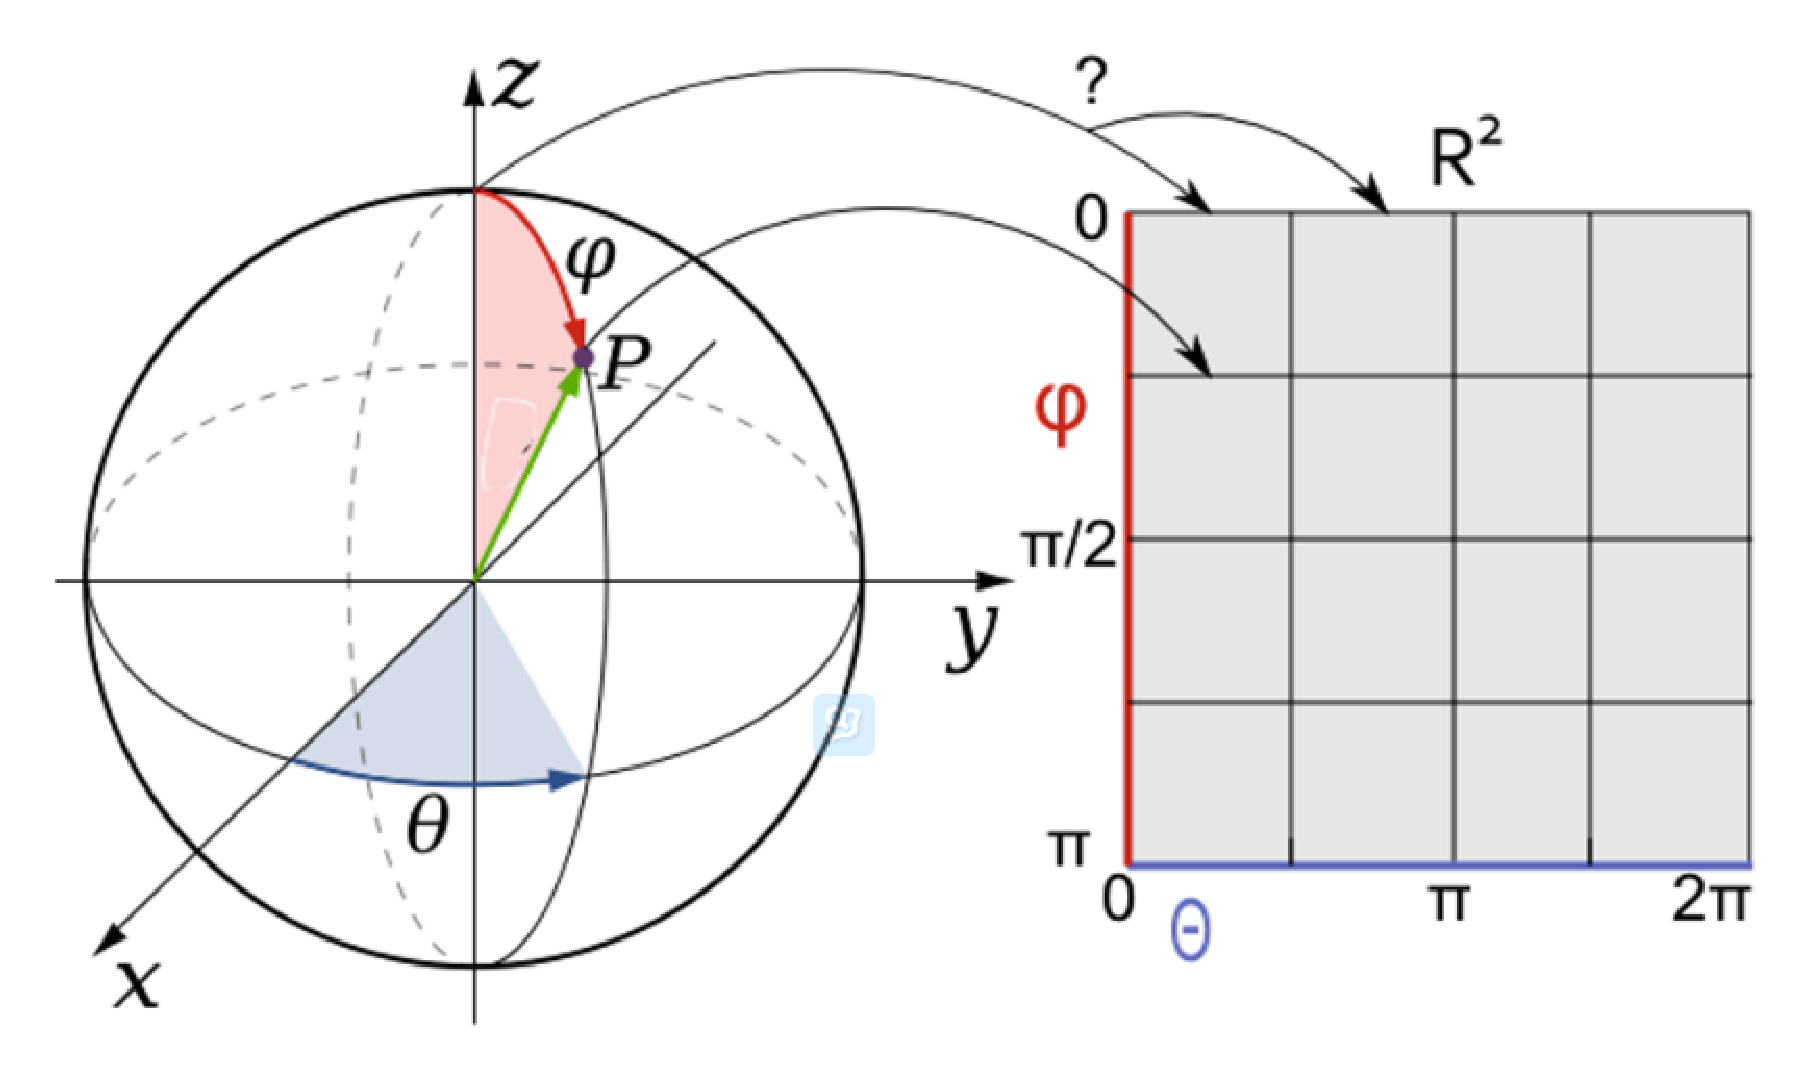
\includegraphics[scale=0.35]{fig3_8.eps}
    \figcaption{从球面的一个邻域到$\mathbb{R}^2$映射的图示}
}
球面上几乎所有的点都可明确地对应于坐标$(\varphi, \theta)$,几乎所有... 但是极点$\varphi = 0$映射到哪儿?不可能有一对一的点,因为极点对应的是一整条线,在上图已经画出。因此球坐标映射不能覆盖整个球面,还需要一个映射将极点及其邻域映射到$\mathbb{R}^2$。相似的问题还出现在$\theta = 0$对应的半圆处,$\theta = 0$与$\theta = 2\pi$映射到$\mathbb{R}^2$的同一个点,因此也不是一一映射。这说明对流形而言,一般不存在一个覆盖流形所有点的全局坐标系,而只有局域坐标系,即仅覆盖某一邻域的坐标系。不过这没关系,因为流形的特征是局部像$\mathbb{R}^n$。

上面说到,球坐标系映射只对开邻域$0 < \varphi < \pi, 0 < \theta < 2\pi$有效,还需要另外的映射来覆盖整个球面。可以使用第二个球坐标系 --- 坐标轴的指向不同,使得有问题的极点不再对应$\varphi = 0$,在第二个映射补充下,球面上所有的点都可映射到$\mathbb{R}^2$,于是2-球面确实是个流形。

流形的平凡例子是$\mathbb{R}^n$,根据定义容易看出。
















